\documentclass[11pt]{article}

\usepackage{listings}
\usepackage{xspace}
\usepackage{amsmath}
\usepackage{eurosym}
\usepackage{amssymb}
\usepackage[pdftex]{graphicx}   

\def\cam{\textsc{cam}\xspace}


\newcounter{myfigure}


\begin{document}
\begin{center}
\huge{SemanticSky} \\ \large{Taking the network up to heaven.}
\end{center}

\tableofcontents
\clearpage

\part{Starfish.}

\section{(The previous project)}

\section{(Results)}



\part{SemanticSky.}

\section{Overview of Semanticsky.}

SemanticSky is a program which, given as input a set of documents, outputs a small multi-agent system where some built-in algorithmic agents try to infer similarity relations (currently, only content/topic similarity) between the input documents.

The main steps through which this is achieved follow:

\begin{itemize}
\item First, each document is transformed into a {\bf Cloud}: an object which theoretically should encapsulate all the information we can extract from the base document. Examples include: names of people mentioned in the document, names of places, statistically frequent word and frequently co-occurring (at a sentence level) pairs of words.
\item  Secondly, these clouds are pairwise evaluated by a list of algorithms called {\bf Guardian Angels} which try to judge their similarity based on different and possibly complementary criteria.
\item Finally, the evaluations of the Guardian Angels are merged into a single one, which represents the final state of the system, at this stage.
\end{itemize}

When the system is first initialized, or when a new document is added to the corpus, this is all there is to it.

But then, some more things will happen, as {\bf Agents} (true people) evaluate by themselves the appropriateness of a link or the relevance of a tag or keyword to some page.

\begin{itemize}
\item The current state of the system is kept under watch on by a supervisor algorithm called {\bf God}, is judged either stable or unsettled. If some part of the network is unsettled, then God waits for more discussion to happen between agents and maybe even fuels it by suggesting relevant links to the parties involved or informing the parties of the presence of a third option, and so on...
\item Once the system settles on some decision, such as the complete relatedness of two items, or maybe even the plain equivalence of two approaches that just happened to go under different names, then God gives feedback to all agents involved (human or algorithmic) regarding the accuracy of their guesses relative to the final state. This way, suggestion-givers who gave bad suggestions will be taken less into account in the future.
\end{itemize}

Crucially, the supervisor algorithm will need to `suspend judgement' on user-backed agents while a discussion is still going on, so that plain democracy will decide on the final state of the system (the objective is to respect people's suggestions, not to distort them) without being influenced by the feedback they received. God is not a moderator: is a plain container and merger of opinions. He listens to the discussion and takes notes. On the other hand it's up to him to judge whether an algorithm is good or not.

Currently it's very easy to implement a new algorithm in the system:

\begin{lstlisting}
import clues
def evaluate(cloud1,cloud2):
	...
	return myevaluation

myalgorithm = clues.algorithms.Algorithm(evaluate)
myguardian = clues.GuardianAngel(myalgorithm)
myguardian.evaluate_all() 
# this will make it evaluate
# all 2-permutations of clouds.
\end{lstlisting}

But not all algorithm are good, and most are good just on very specific subsets of the system. Suppose that we have an algorithm that just checks whether the authors of the document are the same person (and does that by regex matching some query). This algorithm will then return zero for all documents where an 'author' is not defined or the query doesn't match. God then will (try to) understand that the algorithm is useful in some subdomain, even though his average accuracy is very low.

The evaluations that a Guardian Angel performs differ from those of an human agent only in that they are produced automatically. Their route is in fact basically the same: they either get queued and later on processed by God, or (by default) they get immediately processed.

The `processing' implemented is currently quite naive. When an agent has a suspect strong $x$ about the similarity of two documents $y=sim(a,b)$, a ``Clue'' is spawned that conveys the information that the agent has an opinion $x$ about the fact $y$.

Once the clue gets read by God, he will log it and then retrieve all logs about $y$; that is, all the information he has about $y$. Then, he will retrieve all the confidences of the clues (how strongly who produced them believed into them) and the weights (how well their authors usually do at guessing).

The weighted confidences are then averaged, and God's belief about $x$ is updated to the thus obtained value.

Once the system reaches a stable situation about some fact $y$, the supervisor algorithm will hand out feedback to all the algorithms which had some suggestions about $y$ or the discussion surrounding it. We can in fact imagine that, taken any pair of documents, there will be some arguments in favour and some against their similarity or relevance to one another. Not unlike what goes on behind a Wikipedia page (in the 'discussion' section), people will be allowed to debate about various issues, such as pertinence of tags, of links, and in general, let us say, the structure of the network. 
Once the discussion is over (this can be detected by, for example, a month of silence in the discussion page), the system will then adjust the weights of the Guardian Angels' future suggestions. For example, suppose that an algorithm gave particularly good suggestions in this situation (but not in many others); God will then try to guess what is that the algorithm (and maybe even the agent) is good and bad about, and adjust his weights selectively, not unlikely what goes on in the so-called Stacked Generalization models and Mixture of Experts models, which will be discussed later in the Supervisor.Feedback section.

The following sections will try to show in some more details how SemanticSky currently (as of the end of July, 2014) works; starting from the clouds, up to the very heart of this tiny digital pantheon.

\section{Clouds: the bricks.}

At the moment, clouds are more or less simple wrappers for documents. The central data structure for a cloud is what we will call \textbf{layers}. What makes it a simple wrapper is the fact that only the first layer is currently being filled; but the main idea behind a layered cloud is that it should include hierarchically ordered information: from the most precious (and most hardly one-to-one matchable) information to the second-hand, less polished one.

To show the reason behind this few things would do better than an example: suppose we have a document called `Rise and Fall of Ziggy Stardust', containing a couple of pages of history of this man called Ziggy. Unless the title is ironic or in any way misleading, which, assume, is not the case, we already have in front of us a few very important informations: that this document is about a man called Ziggy Stardust and that a rise and a fall are somehow involved.

SemanticSky currently performs little or no semantic analysis, so the cloud will not know that it is Ziggy rising and falling, but just that the names `Ziggy', `rise', `fall' are relevant descriptors of the document. And what's so important about the title is that the mere fact of it being a title tells us that the information stored there is important. This is possible, of course, only because the input data is partly annotated: it's not an uniform body of plain text, but already contains some extra information which we can use. In absence of this, other methods could be used to extract headers, titles and other kind of sources of usually very relevant information.

This is what layers are meant to be for: the innermost layer will certainly contain these four words, plus the most relevant others that, with diverse heuristics, we will be able to extract from the body of the document itself.

Currently, the clouds store just about everything in a single layer, as the information we have is all first-hand: comes directly from the document, which is the most trustworthy source of information we can have at the moment. The layer-building function currently tokenizes everything down to words, stems them (so as to capture the relevance of, say, `learn-', even though in the document the concept appears under many different grammatical forms, which would make the statistical relevance of `learn' by itself very low) and finally produce a list of the pairs of words most frequently co-occurring in sentences.

The sorts of information a cloud currently contains in its only layer are (extracted via regex matching and tokenization):
\begin{itemize}
\item names: all Capitalized Sequences Of Words.
\item urls: all urls either hidden in hrefs (the documents' text is html) or explicitly mentioned in the text.
\item words: information about their frequency (tf) \emph{and} their frequency weighted by their inverse document frequency (tf-idf).
\item core: a special subset of words which we have reasons to believe more important than the other ones; namely those which come from titles or which are labeled as `headline'.
\item tags: a list of the tags assigned to the Starfish item.
\end{itemize}


\subsection{Future work.}

The framework can clearly be expanded even at this level, and time permitting, this will be most certainly one of the most promising directions to go. The layer-based structure is already there, but is not currently used. An immediate expansion of SemanticSky could involve filling the lower-level layers.

Possible sources for the information to fill these layers with include:

\begin{enumerate}
\item The web. The second layer could be filled up, for example, with information drawn from google querying for 'The Rise and Fall of Ziggy Stardust' or some other keywords.
\item Other clouds. At some stage, suppose, the system will settle on the decision that Ziggy's cloud is clearly related (for most of the Starfish users, at least) with (say) David Bowie's cloud. Then, once the confidence about this fact is higher than a certain threshold, we might let some keywords of either clouds `filter' into the lower layers of the other cloud.\footnote{This might have the side effect of forming loops of self-reinforcing feedbacks, so we will have to make sure that algorithms, when re-evaluating the two clouds, won't take into account \emph{that} information as well.}
\item Corpora information. From a corpus search we might discover that `stardust' is very frequently related with Carl Sagan and stars.
\end{enumerate}

The latter example about stars and Carl Sagan is a clear situation where we want to make sure that this information is taken as second-hand only and is given appropriately less weight than the first-hand one.


\section{Agents.}

Agents in Semantic Sky are basically pipes for human input. In Starfish, they will probably be associated with accounts of people who has write access to the Starfish network, but at a more general level, they are `whatever human source of information we have'.

Beside being able to rate similarity of item-pairs, relevance of tags to items, modifying the items, suggesting (removal of) new links or tags, agents are crucial insofar as their discussions and final decisions trigger feedback, which in turn teaches the system what they want. 

Ideally, whenever the system will detect that the discussion about some issue is closed, feedback will trigger and backpropagate to all algorithms (and maybe even agents) that had something to say about it, punishing them for their bad suggestions or rewarding them for the good ones.

The most immediate effect of the feedback is to influence (up or down) the trustworthiness of an agent, be it algorithmic or human in nature.
Trustworthiness is not absolute, however, but relative to some domain or `area of expertise': a person (an algorithm) can be very good on items regarding people but very bad at spotting connections between glossaries and tags. So, we want to learn his expertises and hold as valuable his suggestions in that field, while (proportionately) ignoring his suggestions on topics which we know he is not keen on.

\subsection{Future work.}

Detecting when a discussion is `settled' is not an obvious thing. One could use various `hotness' metrics or functions of the number of people participating to the discussion, the length of their posts and the time gap between them, or more simply the time since the last update of the content of a page. My guess is that some experimental work is needed to find the optimal technique to evaluate when to trigger the feedback: we don't want to increase or decrease trustworthiness of people when the voting is still open (and changes of mind still possible).

Secondly, at the moment feedback is irreversible. This can and should be questioned sometime in the future.




\section{Guardians.}

Guardian Angels are currently the core of the algorithmic part of SemanticSky, and the interaction of them, the Agents and God is probably the theoretically most interesting thing going on there.

Basically, a Guardian is nothing but an agent that only examines pairs of items when prompted (by God) and that takes decisions based on a never changing algorithm.

Their strength is of a collective kind: each of them takes decisions based on a rather small part of all the evidence available, and produces a generally inaccurate (but, on average, above chance) prediction.

Follows a quick description of all the algorithms currently implemented (which is basically their docstring).


\paragraph{tf and tf\_idf\_weighting}

The most standard Guardian Angels, just retrieve the tf / tf-idf value for each word in the bags of words of the documents (also held in the clouds) and returns the cosine of the angle of the two vectorized documents.

\paragraph{naive\_name\_comparison}

Based on the 'names' section of the layers of the clouds, which were previously extracted via regex matching, this algorithm just checks how many names the two clouds share, and normalizes it against the set union of the two lists of names.
The required kind of matching is very strict: a `Ziggy Stardust' in a cloud won't match a `Ziggy, S.' in the other. This could be improved in many ways.

Plus, a name is currently Whatever Is Capitalized, and this is not really so. We are lucky that Starfish does not have pages in German.

Given the little information the algorithm can work on, the 600 nonzero results against 210000 is a reasonable output. Interestingly enough, the algorithm is one of the most precise ones, with a 15\% chance that if he detects something, there is actually something.

\paragraph{extended\_name\_comparison}

This algorithm, as all other algorithms containing the word `extended', is based on the social network principle that if $A$'s friends are $B$'s friends, then $A$ and $B$ are likely to be friends themselves.

Let $names(\phi)$ be the set of names contained in the zero layer of the cloud $\phi$.
Then, for $\phi \in A,B$, we define
\[names(\phi) = \phi.layers[0]['names']\]
\[Neighbours(\phi) = \{a | a \in sky ~ if ~ names(\phi) \cap names(a) \neq \varnothing \}\]
Finally, we make an extended bag of words by summing $\phi$'s names with the cores of all of $\phi$'s neighbours: that is, the most relevant words for all of the clouds which share at least a name with $\phi$. Then, we count the overlaps and normalize against the union of the sets.

Not as precise as naive\_name\_comparison and much more computationally heavy, but gives nonzero results more often.

\paragraph{naive\_core\_overlap}

The same as naive\_name\_comparison, but instead of the `names' entry of the clouds' layers, takes the core, performing a simple \(len(intersection) / len(union)\) computation.

\paragraph{extended\_core\_overlap}

let $C(\psi)$ denote the core of (the zero layer of) some cloud $\psi$. This time, unlike the extended\_name\_overlap algorithm, the words to extend $C(\psi)$ are going to be drawn not directly from other clouds, but from a global repository of the co-occurrence counts of words in sentences based on the whole corpus.

So, the globally most frequently co-occurring pairs, not weighted by idf (which could of course be an interesting extension), go to extend $C(\psi)$ if at least one of the words in the co-occurrence pair is in the core of $\psi$.

So, the extended core of psi $E(C(\psi))$ will be, where $coo(a,b) \iff$ $a$ and $b$ co-occur more than twice in the whole corpus, and $W$ is the set of all words occurring in the corpus:
\[E(C(\psi)) = {w | w \in W \land (w \in C(\psi)\lor \exists b \in C(\psi) : coo(w,b)) }\]

Finally, the two extended cores are compared in the usual intersection / union way.


\paragraph{tag\_similarity\_naive}

This algorithm, as well as the following ones, are made specifically for evaluating the similarity of tag clouds: clouds that wrap tag-type items in Starfish. Typically, the only information we have about this kind of items, beside the name of the tag itself, is a list of synonyms (aliased tags) and perhaps a glossary (a small document). This makes their comparison rather tricky for other algorithms.

Furthermore, there currently are no links in Starfish between tags and other types of items, so we don't have a training set to assess the performance of these algorithms. The choice of treating tag-type items like all other types may also be questioned, but this is not the place for it.

The algorithm, given two clouds, just counts how many pages are tagged with both tags (that is, the tags that the clouds are built around) and normalizes it against the length of the union.

\paragraph{tag\_similarity\_extended}

This algorithm is an instance of a higher-level Guardian Angel, or Meta Angel: to work, it needs some previous evaluation.

Basically, it measures the overlap of the sets of clouds marked with the two tags and returns an averaged confidence of the relations of these links.

Suppose we have the following situation, where $a,b$ are tags (i.e. strings such as `LearningAnalytics',`DavidBowie'):
\begin{enumerate}			
\item[$a\to$] [cloud1, cloud2]; that is: both cloud1 and cloud2 are tagged with `$a$'.
\item[$b\to$] [cloud1, cloud3]
\item[$c\to$] [cloud4,	cloud5]
\end{enumerate}

Clearly, similarity(cloud1,cloud1) = 1, so tag $a$ and $b$ will be at least 0.5 related since they share half of their clouds; more if cloud2 and cloud3 are related in gods' beliefs.
Then suppose cloud1 and cloud4 are believed to be related by 0.4, and cloud5, cloud2, are related by 0.6, but cloud5 and cloud3 are totally unrelated.
Then, tag c will be much closer to tag a than to tag b.

The algorithm just computes over this intuition.

\paragraph{tag\_overlap}
This algorithm, unlike the two previous ones, is a measure of the distance of two nontag-type clouds, and simply measures the intersection/union of the tags of the two clouds.


\paragraph{coo\_dicts\_overlap}

This algorithm has two versions, plus a third one which consists simply in taking the best result from v1 and v2.

\subparagraph{v1} This version returns a pair-to-pair correspondence check of co-occur\-ring pairs of words in the two clouds. Such correspondence is very valuable, but rare.

\subparagraph{v2} This version is more permissive (returns many more nonzero values) and consists in splitting the pairs thereby using single words as term of comparison. (Basically it performs a bag of words overlap/union, building the bags from the co-occurrence dictionary). Implements Grefenstette (1994) algorithm for computing the values.

\paragraph{coo\_dicts\_neighbour}

Taken the co-occurring pairs in cloud $\phi$, denoted $coo(\phi)$, we split them and augment this bag of words with the most frequent words that often co-occur with them at the whole corpus level. (Similar to extended\_core\_overlap), but based on a different starting set. Then compares the two extended bags.

\paragraph{coo\_dicts\_extended\_neighbour}

This algorithm is very complex, takes ages to run and is so permissive that it captures far more noise than signal. Probably garbage.


\subsection{Future work.}
~

$\bullet \quad$Guardian Angels are cool, but they also are currently very stupid. Each one of them just performs a little task in a probably very naive way: this could be improved (but, on the other hand, the main idea behind ensembles is precisely a large number of very stupid algorithms that collectively produce a very smart decision. Be it their small number or their being too stupid, currently this doesn't happen so much). Thus, we could either increment their number (boosting is an option) or make them smarter.

$\bullet \quad$Plus, the more and most diverse the angels' decision algorithm are, the higher the overall performance of the system will be. Currently, there are bunches of three-to-four algorithms that perform very similar computations (and mostly work on the same evidence). Thus, one immediate way to extend the system will be to implement more guardians, or to add variations to the already existing ones.

$\bullet \quad$As noticed above, also, the decisions of the algorithms which are currently implemented are based on a rather small subset of all the available information. Some algorithm only takes into account the words' frequency, some other the words' idf-frequency, some other just the `names' appearing in the text, and so on. Some effort might be put into smarter algorithms able to combine on the fly all these different types of inputs, or to extend the range of inputs available, such as through web crawling\footnote{
A first attempt in this direction has already been made: I constructed an algorithm which would, given a pair of words $a,b$, retrieve the number of google hits for the query ``NEAR($a,b$)|NEAR($a,b$)'', later normalizing it with the number of hits for queries containing just the single words $a$ and $b$. To do the same with clouds is not as straightforward and will need some more research and might involve, for example, keyword extraction (from other Angels' evaluations, maybe).}.

$\bullet \quad$Another thing which might change is that currently algorithms don't (strictly speaking) learn anything. They just go on spitting the same decisions over and over, and is a higher-level algorithm that is delegated the work of gating their decisions so that they get their weight appropriately with respect to their usual worth. An attempt could be made to include amongst this kind of algorithm some more standard learners, such as neural networks.

$\bullet \quad$Finally, the Guardians' reach could be much extended by having them evaluate not only pairs of clouds but also single clouds, or larger groups. An algorithm for example might try to find hubs in the network, or islands that might then be addressed by `bridging' attempts. Suppose for example that there is a rather insulated part of the network that is rather inaccessible from the external world. not only that is an interesting information by itself, but also we may want to fuel discussion by, for example, suggesting more links to `external' clouds or by giving incentives to those who propose such links.\footnote{A sketch of higher-level Guardian Angels, which I called Meta Angels, is already present but has currently not been tested or used. In this case, the meta angel tries to use evaluations as they come out of the lower-level angels and take them further: given two items $x,y$ the meta angel's evaluation is a function of how many neighbours $x$ and $y$ share (weighted clearly by how near they are) in the current state of the system.}

\section{The Supervisor.}

The Supervisor, also called God, is a gating machine that mediates between the angels and the final output of the system, doing the mostly bureaucratic work of gathering the judgements of the algorithms and agents involved in some voting and weighting them up or down according to the source's trustworthiness, finally merging them (by averaging) into a conclusive judgement that goes to build a belief state.

Such belief state is the final outcome of the system, and represents a snapshot of the link structure within Starfish according to the system. Ideally, we want such structure to closely match Starfish's own link structure (the links that physically appear in the pages) that currently have been hand-hard-wired there by physical persons.

But, as Starfish is planned to be a dynamical network, where many discussions are open-ended and there is not always a clear yes/no answer to all questions, we won't pretend Semantic Sky to aim at that goal either. Its highest-rated beliefs should of course have a strong correspondence with the actual structure of Starfish, but the whole body of the iceberg (hidden for example through some thresholding) can be open-ended as much as the underlying discussion (carried out by humans in parallel) is.

These considerations, among others, led us to the conclusion that recall is not a priority for Semantic Sky neither as a suggestions machine nor as a link-spotter in general, making it somewhat closer to a ranker.

The fact that there is a centralised object gating the outputs of several other objects (partly algorithmic, but mostly human) makes Semantic Sky close to what goes under the label of `ensemble methods'.

More specifically, we found the closest neighbours of Semantic Sky in the literature to be the \emph{mixture of experts} methods and the \emph{stacked generalization model} models.\footnote{For terminology and explanations, see for example [Introduction to machine learning, 2nd ed. Ethem Alpaydin, pp. 434-435].}

Also, some intuitions behind SemanticSky can be traced back to Neural Networks and / or Bayesian Network, with respect to which the major difference is that the neurons do not just transform the signal but actually produce it, and are not simple (though fuzzy) logic gates but are complex algorithms.

\subsection{Future work.}

When some agent (or a Guardian) communicates to God a new decision concerning some item $x$, God's belief state is updated by the classical formula 
\[new\_value = previous\_value - [(previous\_value - new\_value) * learning\_rate] \]
and nothing more. Some efforts need to be put in determining whether this is the best strategy available. Through the mechanism of contextualized trustworthiness, angels themselves repress their own decisions based on the feedback they received, but this might not be enough, or there just might be more. Maybe some angel's decisions are just all wrong, or maybe it produces such good decisions that even though his confidence in them with trustworthiness at 1 is still not at all high, we might want to boost artificially his confidence: to hear more than we listen to, so to say. God itself might learn, in other words, some useful way of transforming the output to match the current state of the system, thereby minimising his regrets directly (instead of relying entirely on the angel's own learning mechanisms.).

%Also, maybe something interesting would happen if God would be able to group similar angels making them a single voter with a proportionally higher impact on his decisions.

\section{Conclusions}

In this section we are going to discuss what we learned while working on SemanticSky.
First, we will show some graphical and numerical results, in an attempt to evaluate how the system performs, therewith explaining why the results are what they are and not otherwise.

The main test we run consists in removing all the clouds from the sky and initializing an empty God on such empty sky. Then, we add them back one by one\footnote{Or, to reduce the running time of the test, a bunch of them per time. In fact, the tests I ran mostly were made with step 5 and 6. This has also the effect of reducing the amount of memory used (by $1/n$th) for $n$ = step. And given that for step 6 it's still $74mb$, this is necessary.} and we ask all the guardians to evaluate the whole sky; that is: to assess all similarities they can spot between the present clouds. 
Finally, the Knower (a training algorithm that `knows the truth') judges on their evaluations and triggers feedback, adjusting the trustworthiness of the angels in the various contexts.

\subsection{Testing: online evaluation.}

First I will write down clearly and discuss, where needed, the parameters I used for the test; then show the results.

$\bullet \quad$ Learning rate $= 0.4$.

$\bullet \quad$ Punish = False. This means that guardians don't receive negative feedback for links that are not in the knower's database of `truths'.\footnote{In a real-life application of Semantic Sky this will be a nonexisting issue, but in a test, we have to choose which items we give negative feedback to. In this test I chose not to give negative feedback for all links currently not in Starfish and mistakenly captured by the guardians as similar. For further discussion and a test with punish True, see Appendix .}

To state this more clearly: guardians receive feedback only on items in the knower's database = Starfish's database. The valuation they get for some link, namely, is $1 - $ their current rating of the link.

$\bullet \quad$ Step = 6: clouds were added back to the sky 6 by 6.

$\bullet \quad$ Update rule = median of all feedbacks. The current trustworthiness of some angel relative to some link type (person-to-person, question-to-answer...) is the \emph{median} of all the feedback he has ever received about links with that link type. \footnote{Other available solutions include averaging \[(sum(all feedbacks)/ len(all feedbacks))\] and step-by-step averaging \[(value = (previous value + value) / 2)\], plus average and median of the last $n$ items.}

$\bullet \quad$ Merging rule. This affects how the new suggested value (as computed by the update rule) is merged with the previous one. Extremes include ignoring it and replacing the latter with the former. The standard merge is:
\[new\_value = previous\_value - [(previous\_value - new\_value) * learning\_rate] \]

This is, sampled at each loop of the test, the average value of each Angel's beliefs in all true links; that is, all the links that according to our training set (represented by the knower) are truly out there.

We can see how the values increase and (seem to) stabilize for most angels after around 45 iterations. This means that there were $270$ clouds (since the step was 6) in the sky at that point. The least stable lines represent the angels which have very little nonzero evaluations, and thus receive less feedback.

\stepcounter{myfigure}
\def\svgwidth{550pt}
\begingroup%
  \makeatletter%
  \providecommand\color[2][]{%
    \errmessage{(Inkscape) Color is used for the text in Inkscape, but the package 'color.sty' is not loaded}%
    \renewcommand\color[2][]{}%
  }%
  \providecommand\transparent[1]{%
    \errmessage{(Inkscape) Transparency is used (non-zero) for the text in Inkscape, but the package 'transparent.sty' is not loaded}%
    \renewcommand\transparent[1]{}%
  }%
  \providecommand\rotatebox[2]{#2}%
  \ifx\svgwidth\undefined%
    \setlength{\unitlength}{1229.4bp}%
    \ifx\svgscale\undefined%
      \relax%
    \else%
      \setlength{\unitlength}{\unitlength * \real{\svgscale}}%
    \fi%
  \else%
    \setlength{\unitlength}{\svgwidth}%
  \fi%
  \global\let\svgwidth\undefined%
  \global\let\svgscale\undefined%
  \makeatother%
  \begin{picture}(1,0.50366032)%
    \put(-0.18,0.12){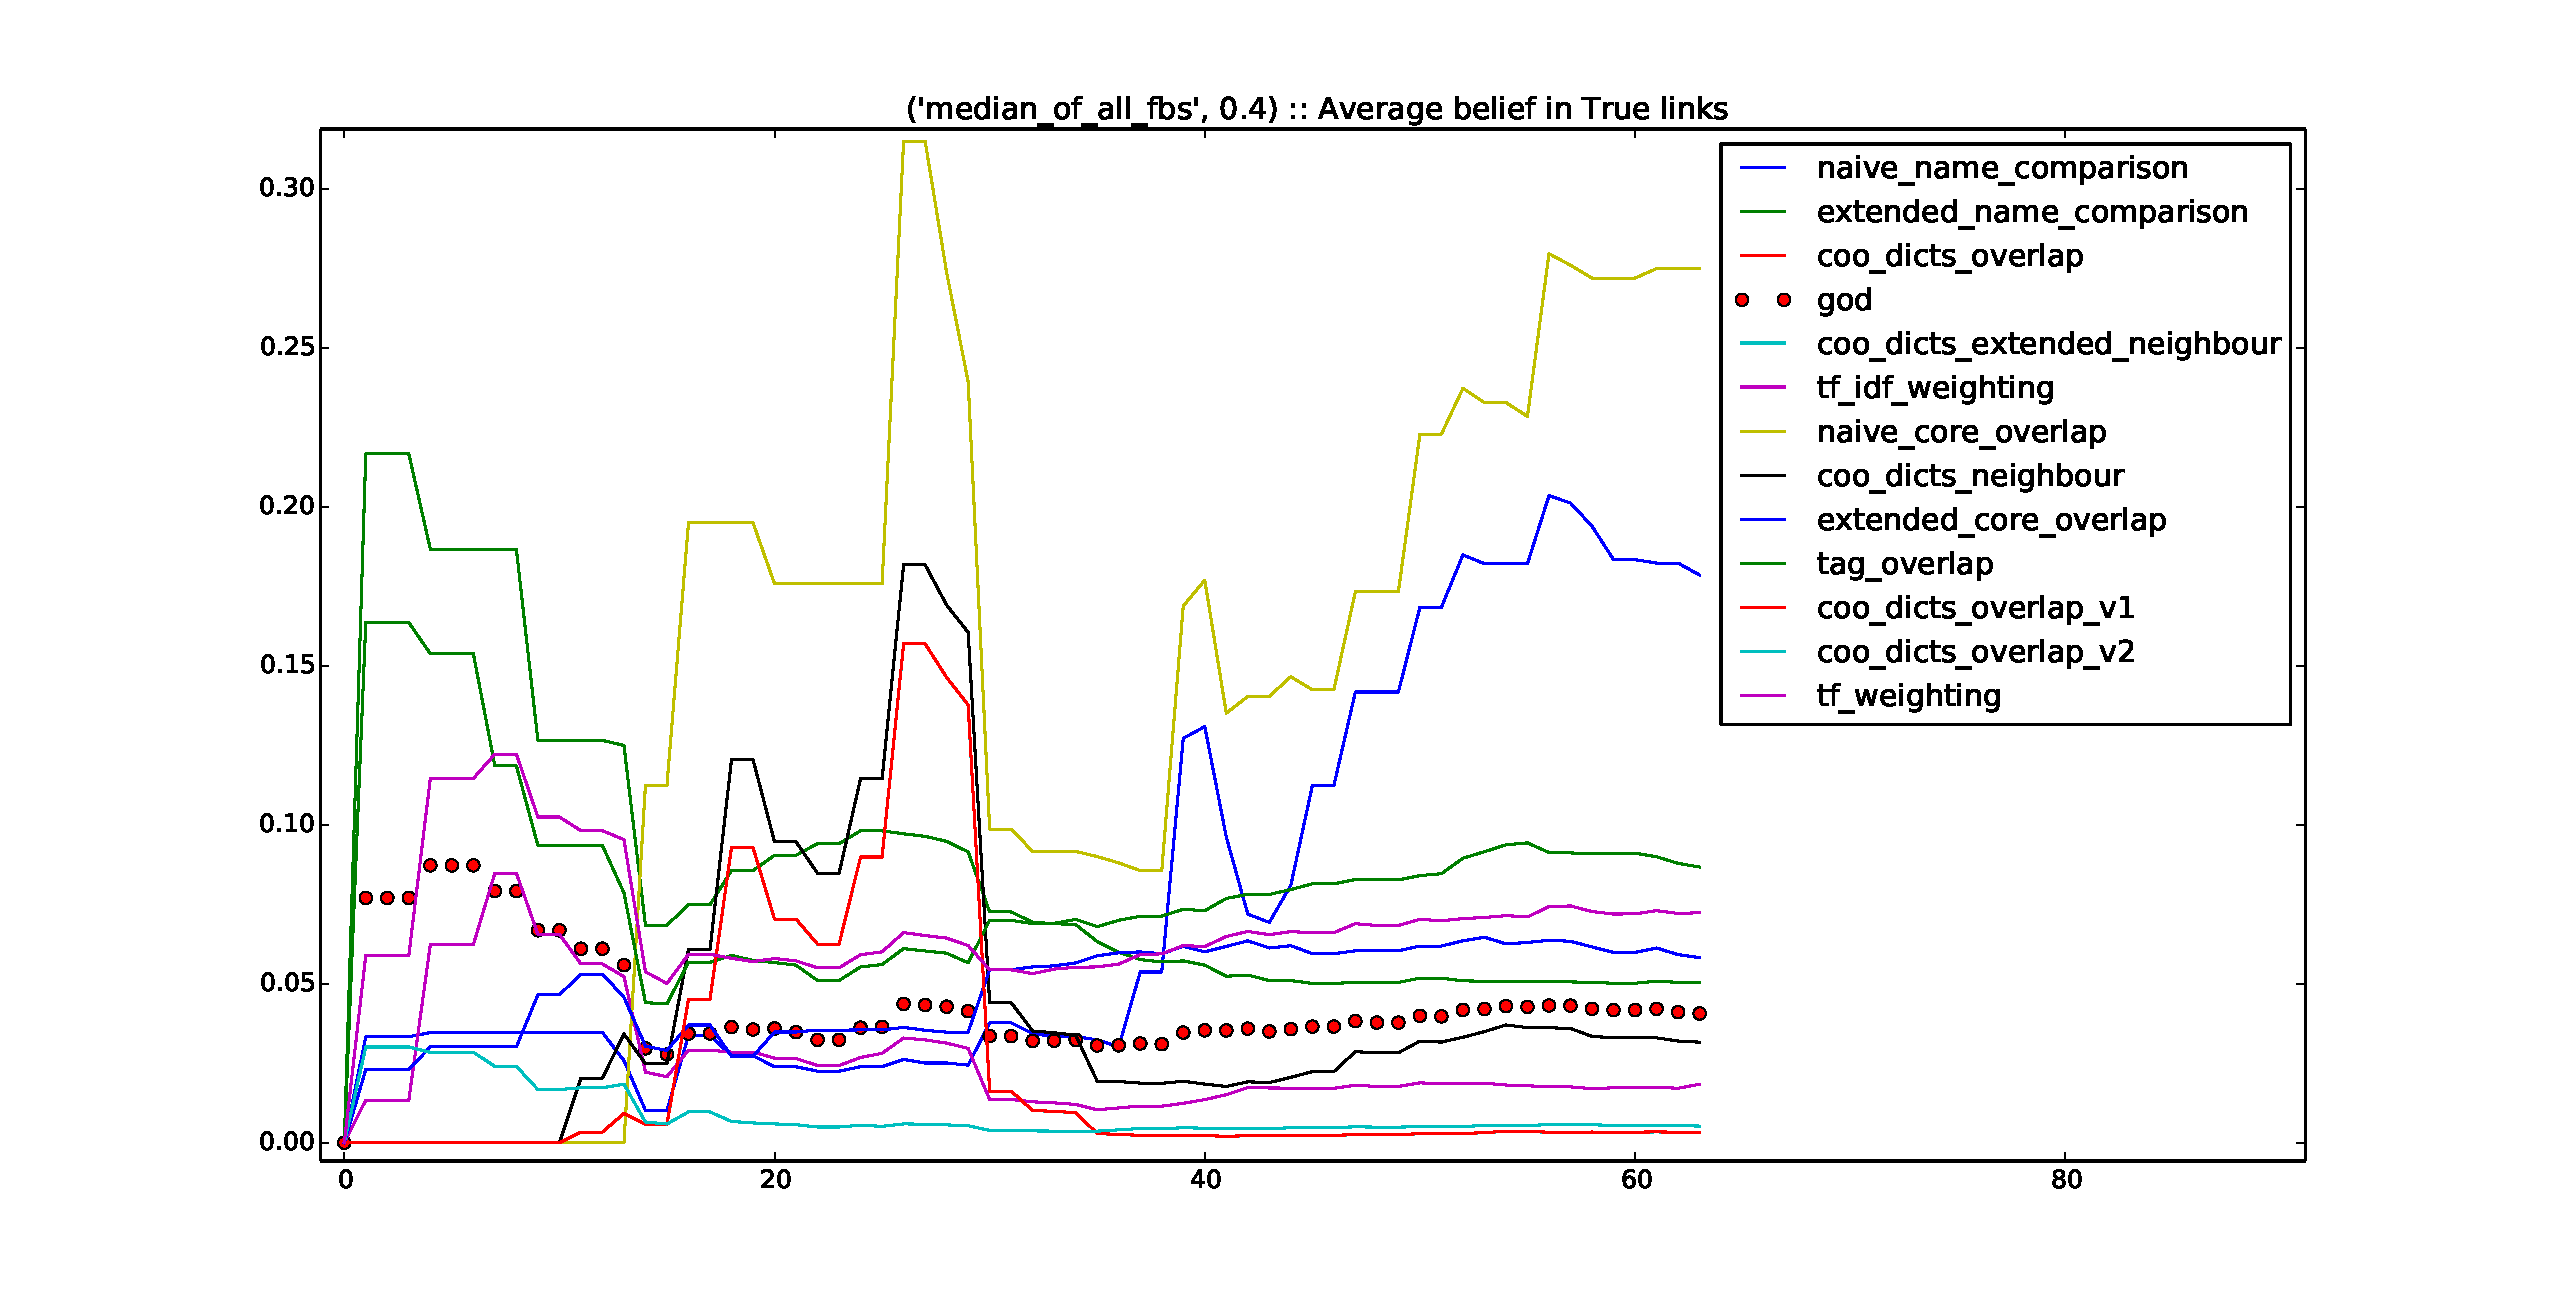
\includegraphics[width=\unitlength]{/home/pietro/Perceptum/code/starfish/similarity/SemanticSky/report_imgs/belief_in_true_links.pdf}\hspace{-355pt} Figure \themyfigure: belief in true links}%
  \end{picture}%
\endgroup%
\vspace{5pt}

As the test proceeds, the values quickly stabilize around (an average of) 0.05, represented quite accurately by God's line. Note that God's belief set is a weighted average, not a plain one.

Figure 2 shows the progression of average beliefs in false links: that is, links that are currently not in Starfish. The convergence in this case is much faster because there are many more false links than true ones.

\stepcounter{myfigure}
\def\svgwidth{550pt}
\begingroup%
  \makeatletter%
  \providecommand\color[2][]{%
    \errmessage{(Inkscape) Color is used for the text in Inkscape, but the package 'color.sty' is not loaded}%
    \renewcommand\color[2][]{}%
  }%
  \providecommand\transparent[1]{%
    \errmessage{(Inkscape) Transparency is used (non-zero) for the text in Inkscape, but the package 'transparent.sty' is not loaded}%
    \renewcommand\transparent[1]{}%
  }%
  \providecommand\rotatebox[2]{#2}%
  \ifx\svgwidth\undefined%
    \setlength{\unitlength}{1229.4bp}%
    \ifx\svgscale\undefined%
      \relax%
    \else%
      \setlength{\unitlength}{\unitlength * \real{\svgscale}}%
    \fi%
  \else%
    \setlength{\unitlength}{\svgwidth}%
  \fi%
  \global\let\svgwidth\undefined%
  \global\let\svgscale\undefined%
  \makeatother%
  \begin{picture}(1,0.50366032)%
    \put(-0.18,0){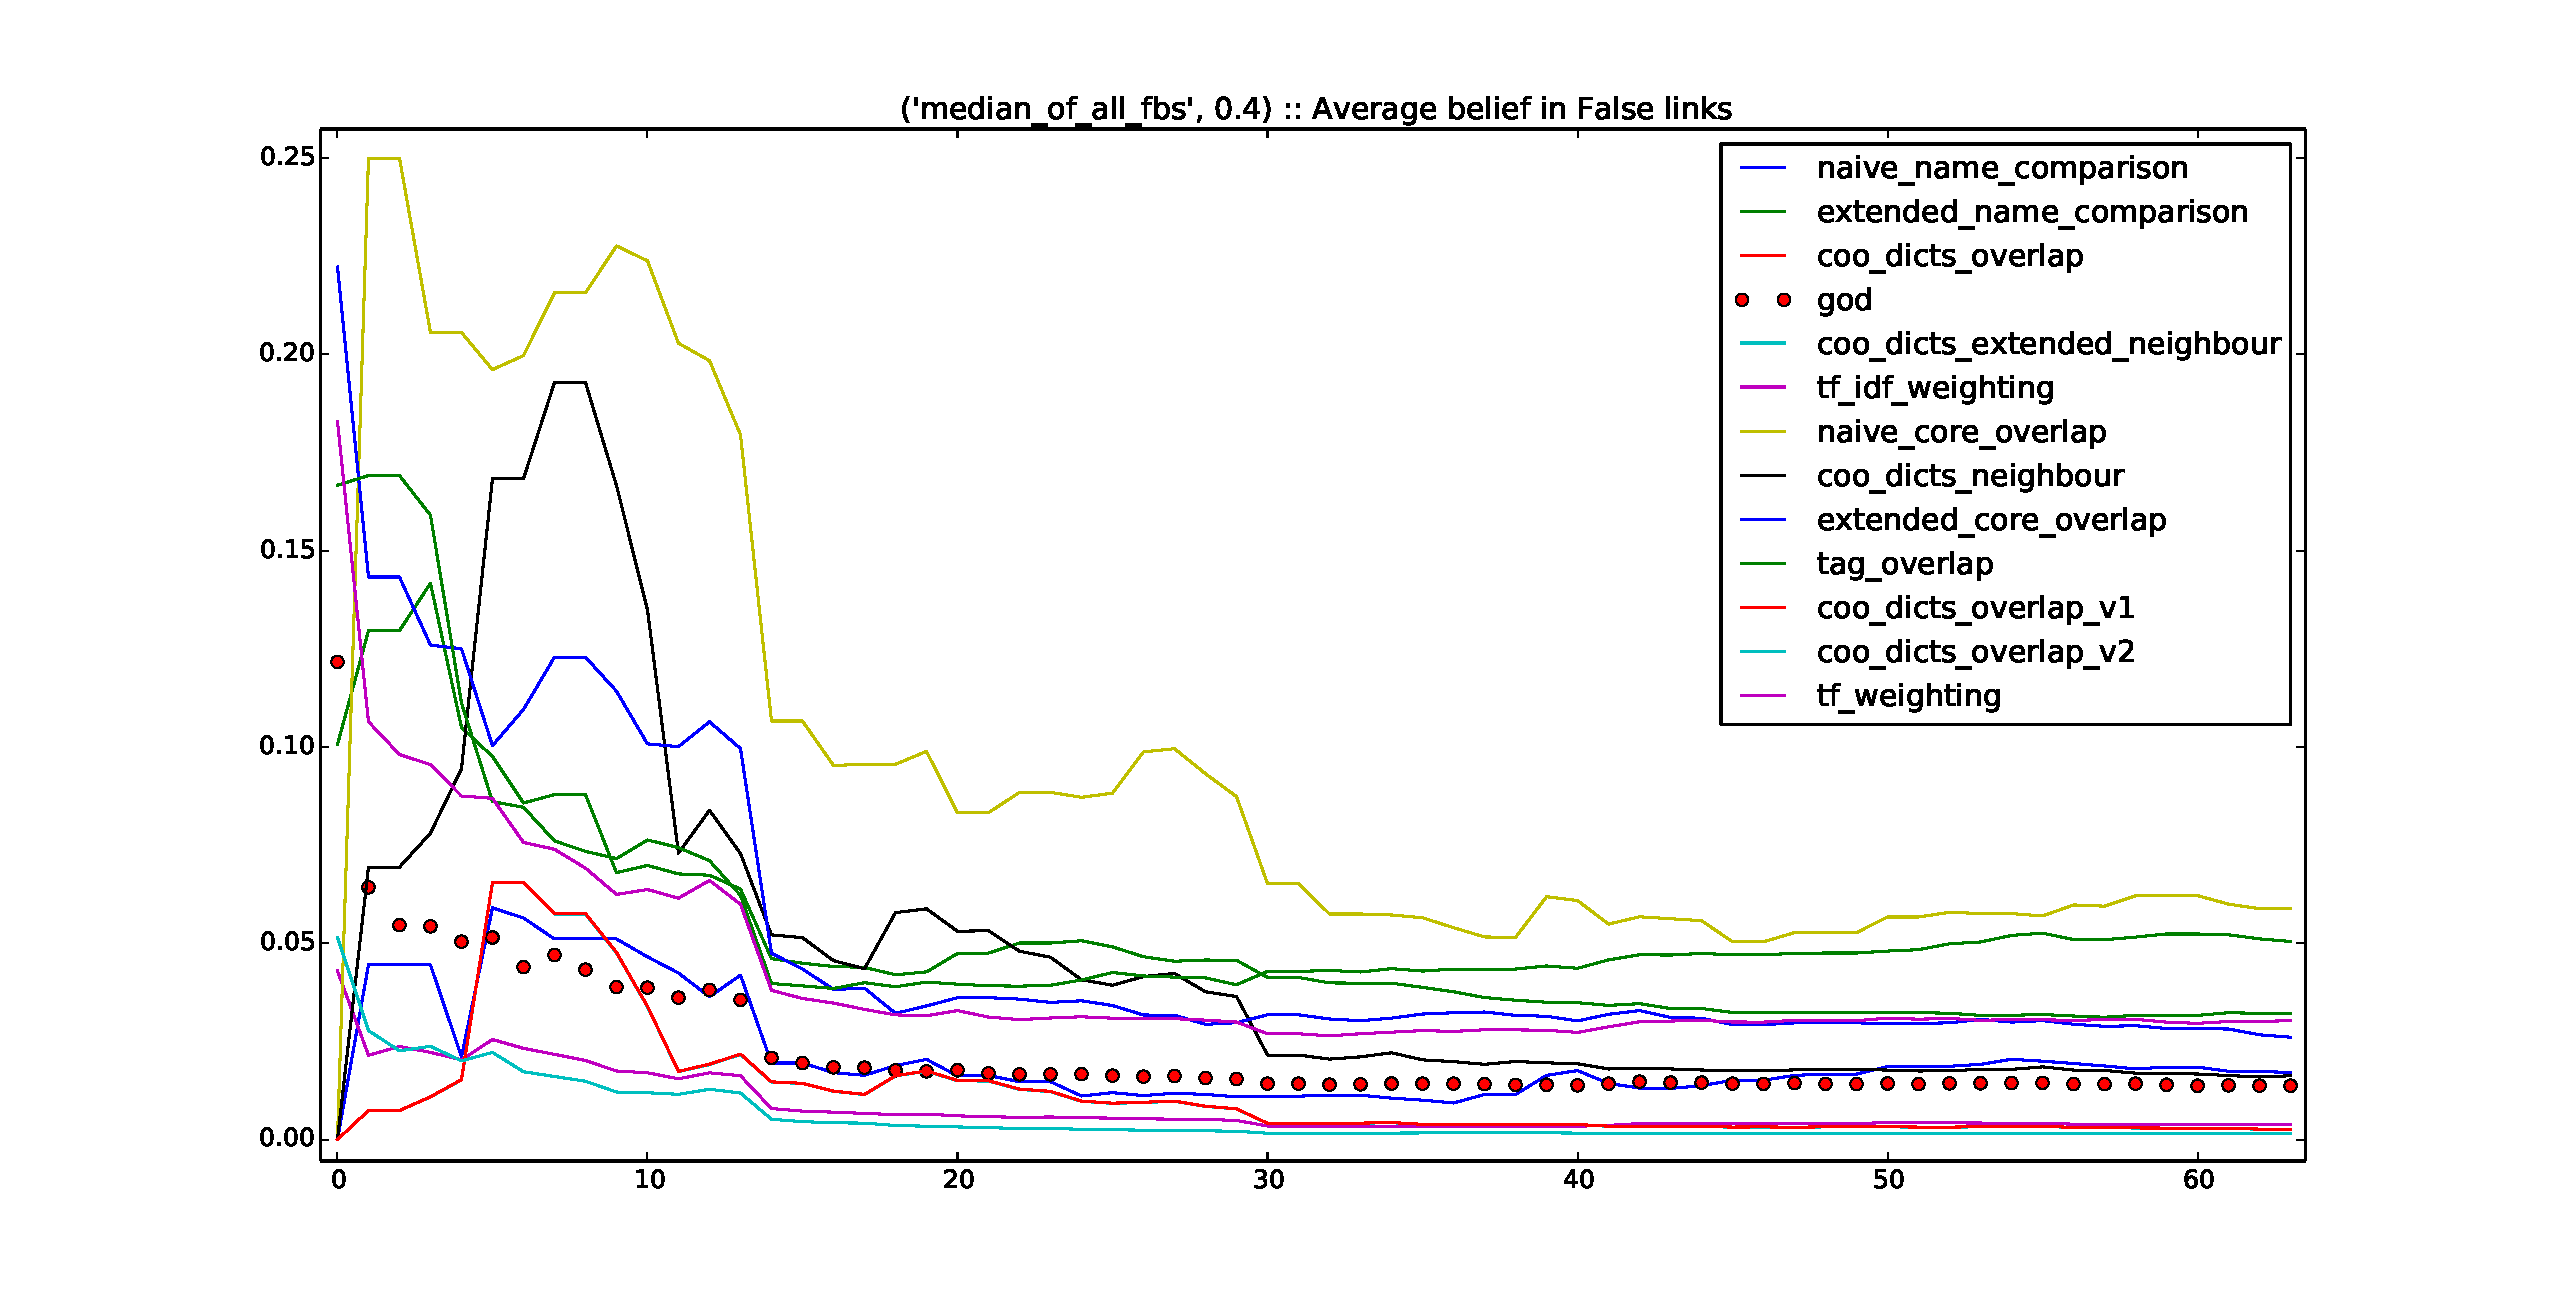
\includegraphics[width=\unitlength]{/home/pietro/Perceptum/code/starfish/similarity/SemanticSky/report_imgs/belief_in_false_links.pdf}\hspace{-355pt} Figure \themyfigure: belief in false links}%
  \end{picture}%
\endgroup%
\vspace{5pt}
Finally, these are the (non-cumulative) regrets of all angels and God itself.

\stepcounter{myfigure}
\def\svgwidth{450pt}
\begingroup%
  \makeatletter%
  \providecommand\color[2][]{%
    \errmessage{(Inkscape) Color is used for the text in Inkscape, but the package 'color.sty' is not loaded}%
    \renewcommand\color[2][]{}%
  }%
  \providecommand\transparent[1]{%
    \errmessage{(Inkscape) Transparency is used (non-zero) for the text in Inkscape, but the package 'transparent.sty' is not loaded}%
    \renewcommand\transparent[1]{}%
  }%
  \providecommand\rotatebox[2]{#2}%
  \ifx\svgwidth\undefined%
    \setlength{\unitlength}{1229.4bp}%
    \ifx\svgscale\undefined%
      \relax%
    \else%
      \setlength{\unitlength}{\unitlength * \real{\svgscale}}%
    \fi%
  \else%
    \setlength{\unitlength}{\svgwidth}%
  \fi%
  \global\let\svgwidth\undefined%
  \global\let\svgscale\undefined%
  \makeatother%
  \begin{picture}(1,0.50366032)%
    \put(-0.12,0){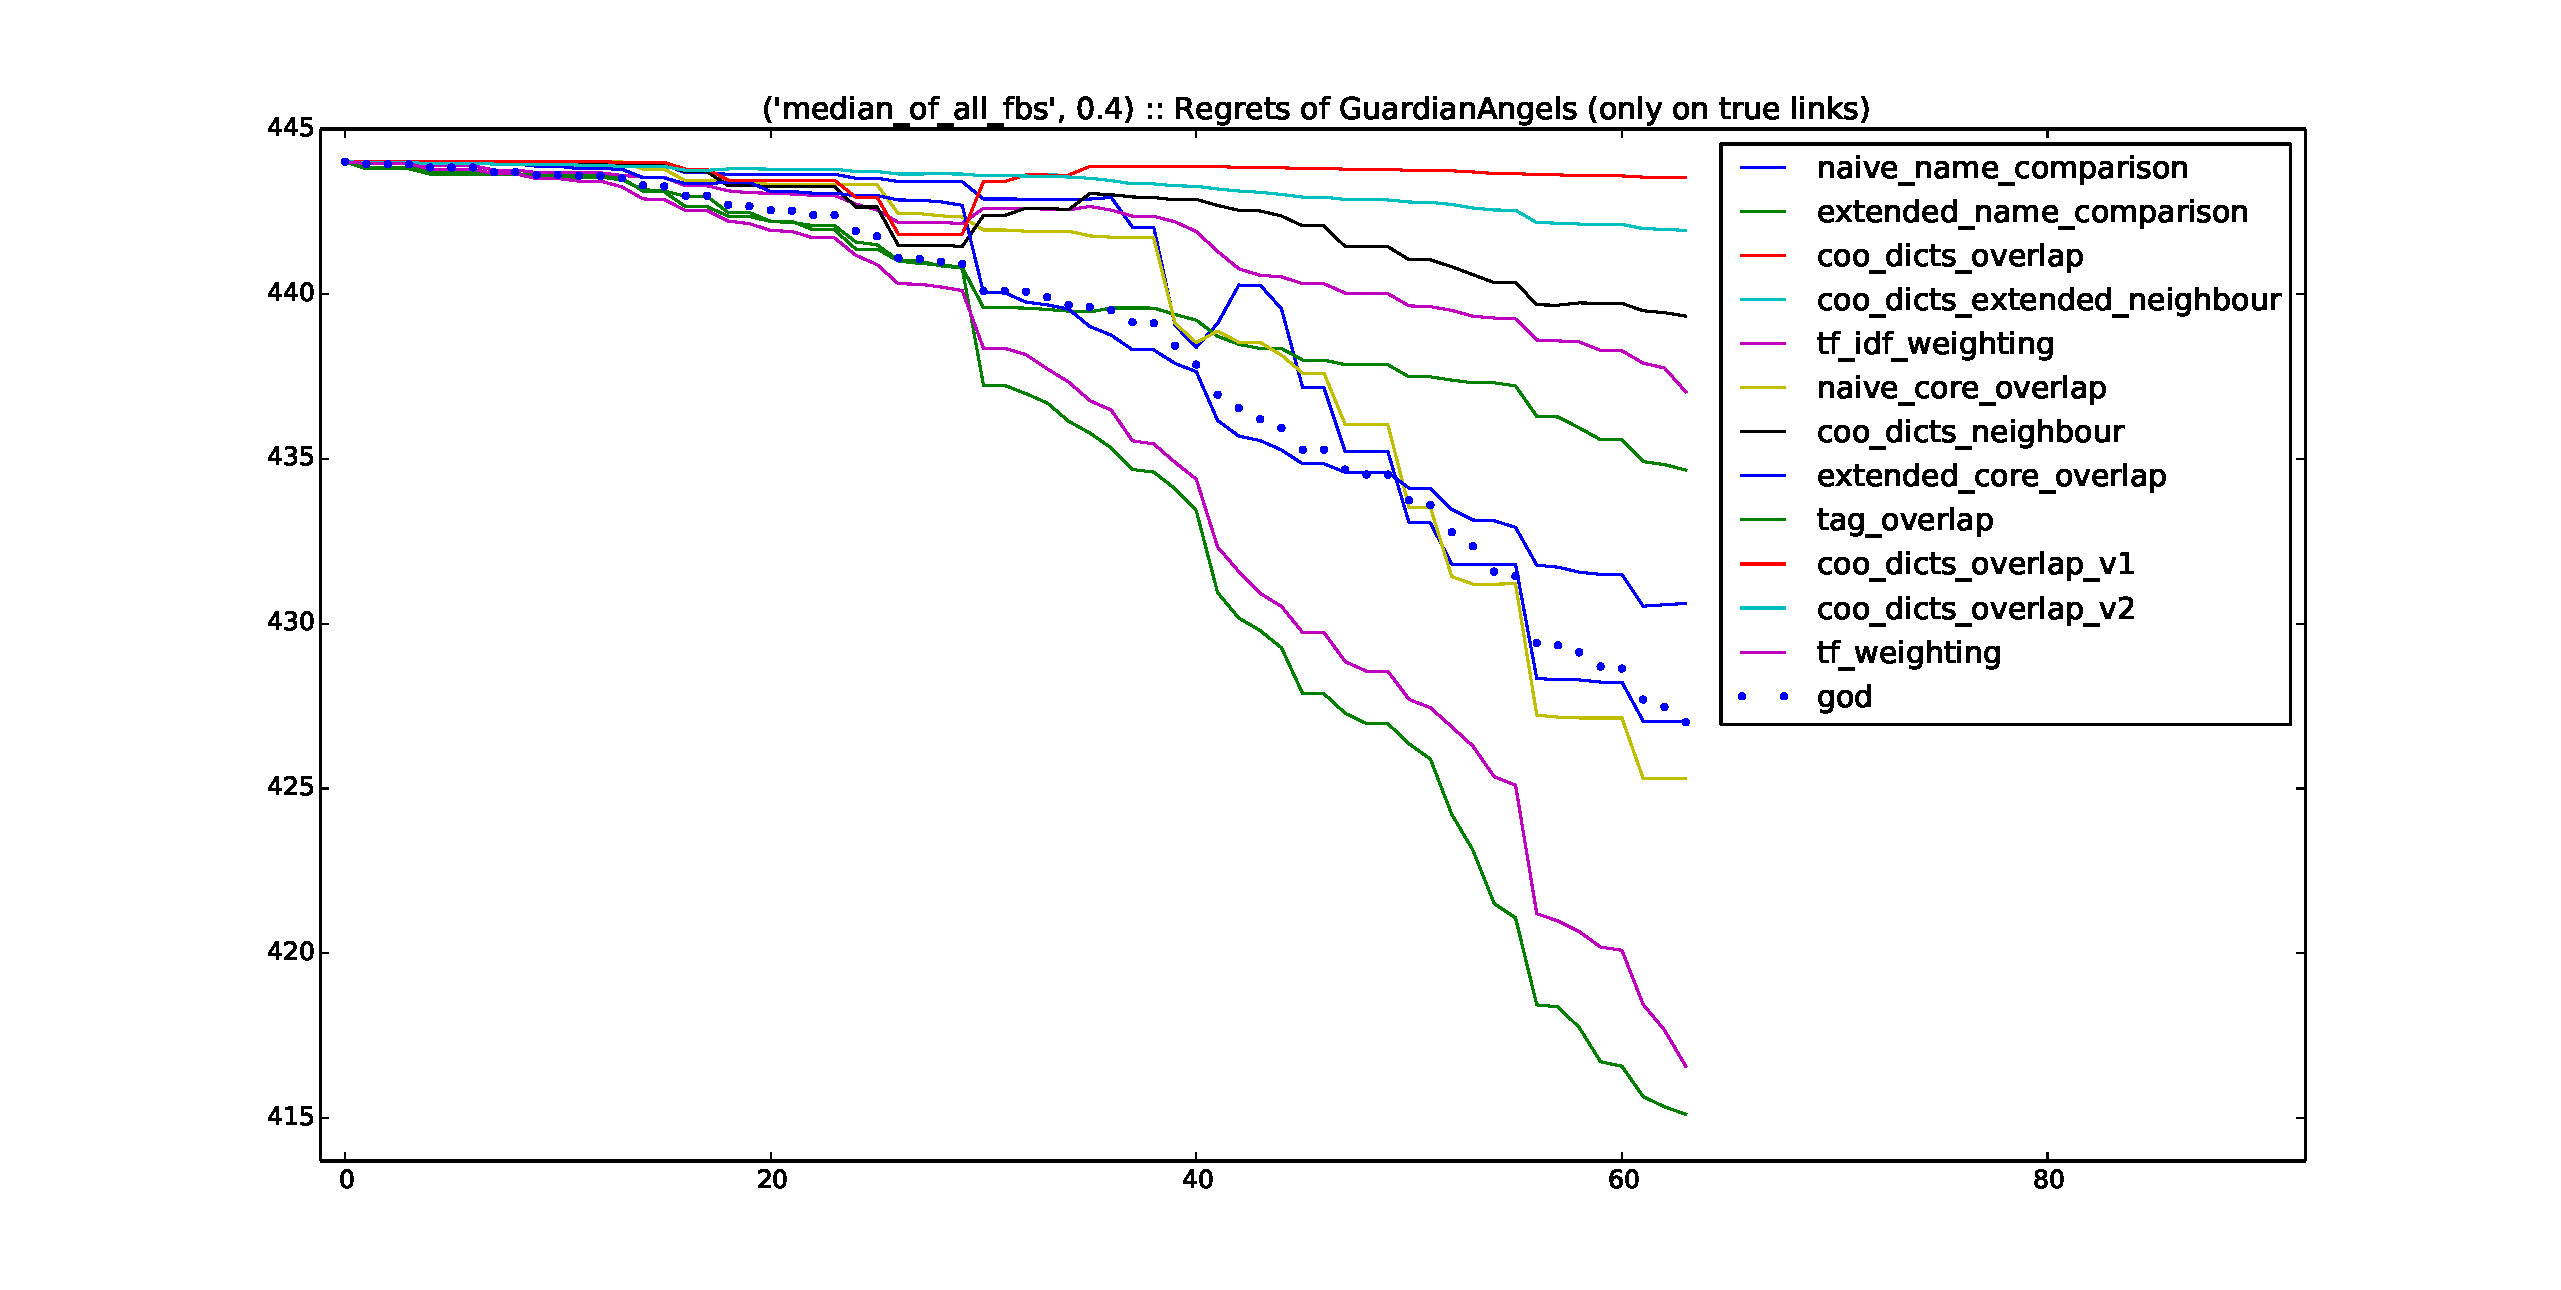
\includegraphics[width=\unitlength]{/home/pietro/Perceptum/code/starfish/similarity/SemanticSky/report_imgs/regrets_ontrue.pdf}
    \hspace{-300pt} Figure \themyfigure: regrets on true links }%
  \end{picture}%
\endgroup%
\vspace{5pt}
Regret (for angel $A$) was computed as follows: $sum$($(1 - A.belief\_in(x))$ for $x$ in $all\_truths$ ), where $all\_truths$ is a list of all links actually existing in Starfish (that is: the Knower's database).

The angels whose regrets don't decrease are the tag-similarity angels (hidden for clarity's sake in the next plots). Currently lacking Starfish any data about how similar two tags are, no link of that type (tag-to-tag) is available in Starfish, and all the feedback will be negative.

One nice thing to notice is that all the algorithms' regret increment is stably decreasing: there is no faulty learner.
Although, the regrets computed on all links (and not only on true ones) reveals a different picture:

\stepcounter{myfigure}
\def\svgwidth{450pt}
\begingroup%
  \makeatletter%
  \providecommand\color[2][]{%
    \errmessage{(Inkscape) Color is used for the text in Inkscape, but the package 'color.sty' is not loaded}%
    \renewcommand\color[2][]{}%
  }%
  \providecommand\transparent[1]{%
    \errmessage{(Inkscape) Transparency is used (non-zero) for the text in Inkscape, but the package 'transparent.sty' is not loaded}%
    \renewcommand\transparent[1]{}%
  }%
  \providecommand\rotatebox[2]{#2}%
  \ifx\svgwidth\undefined%
    \setlength{\unitlength}{1229.4bp}%
    \ifx\svgscale\undefined%
      \relax%
    \else%
      \setlength{\unitlength}{\unitlength * \real{\svgscale}}%
    \fi%
  \else%
    \setlength{\unitlength}{\svgwidth}%
  \fi%
  \global\let\svgwidth\undefined%
  \global\let\svgscale\undefined%
  \makeatother%
  \begin{picture}(1,0.50366032)%
    \put(-0.12,0){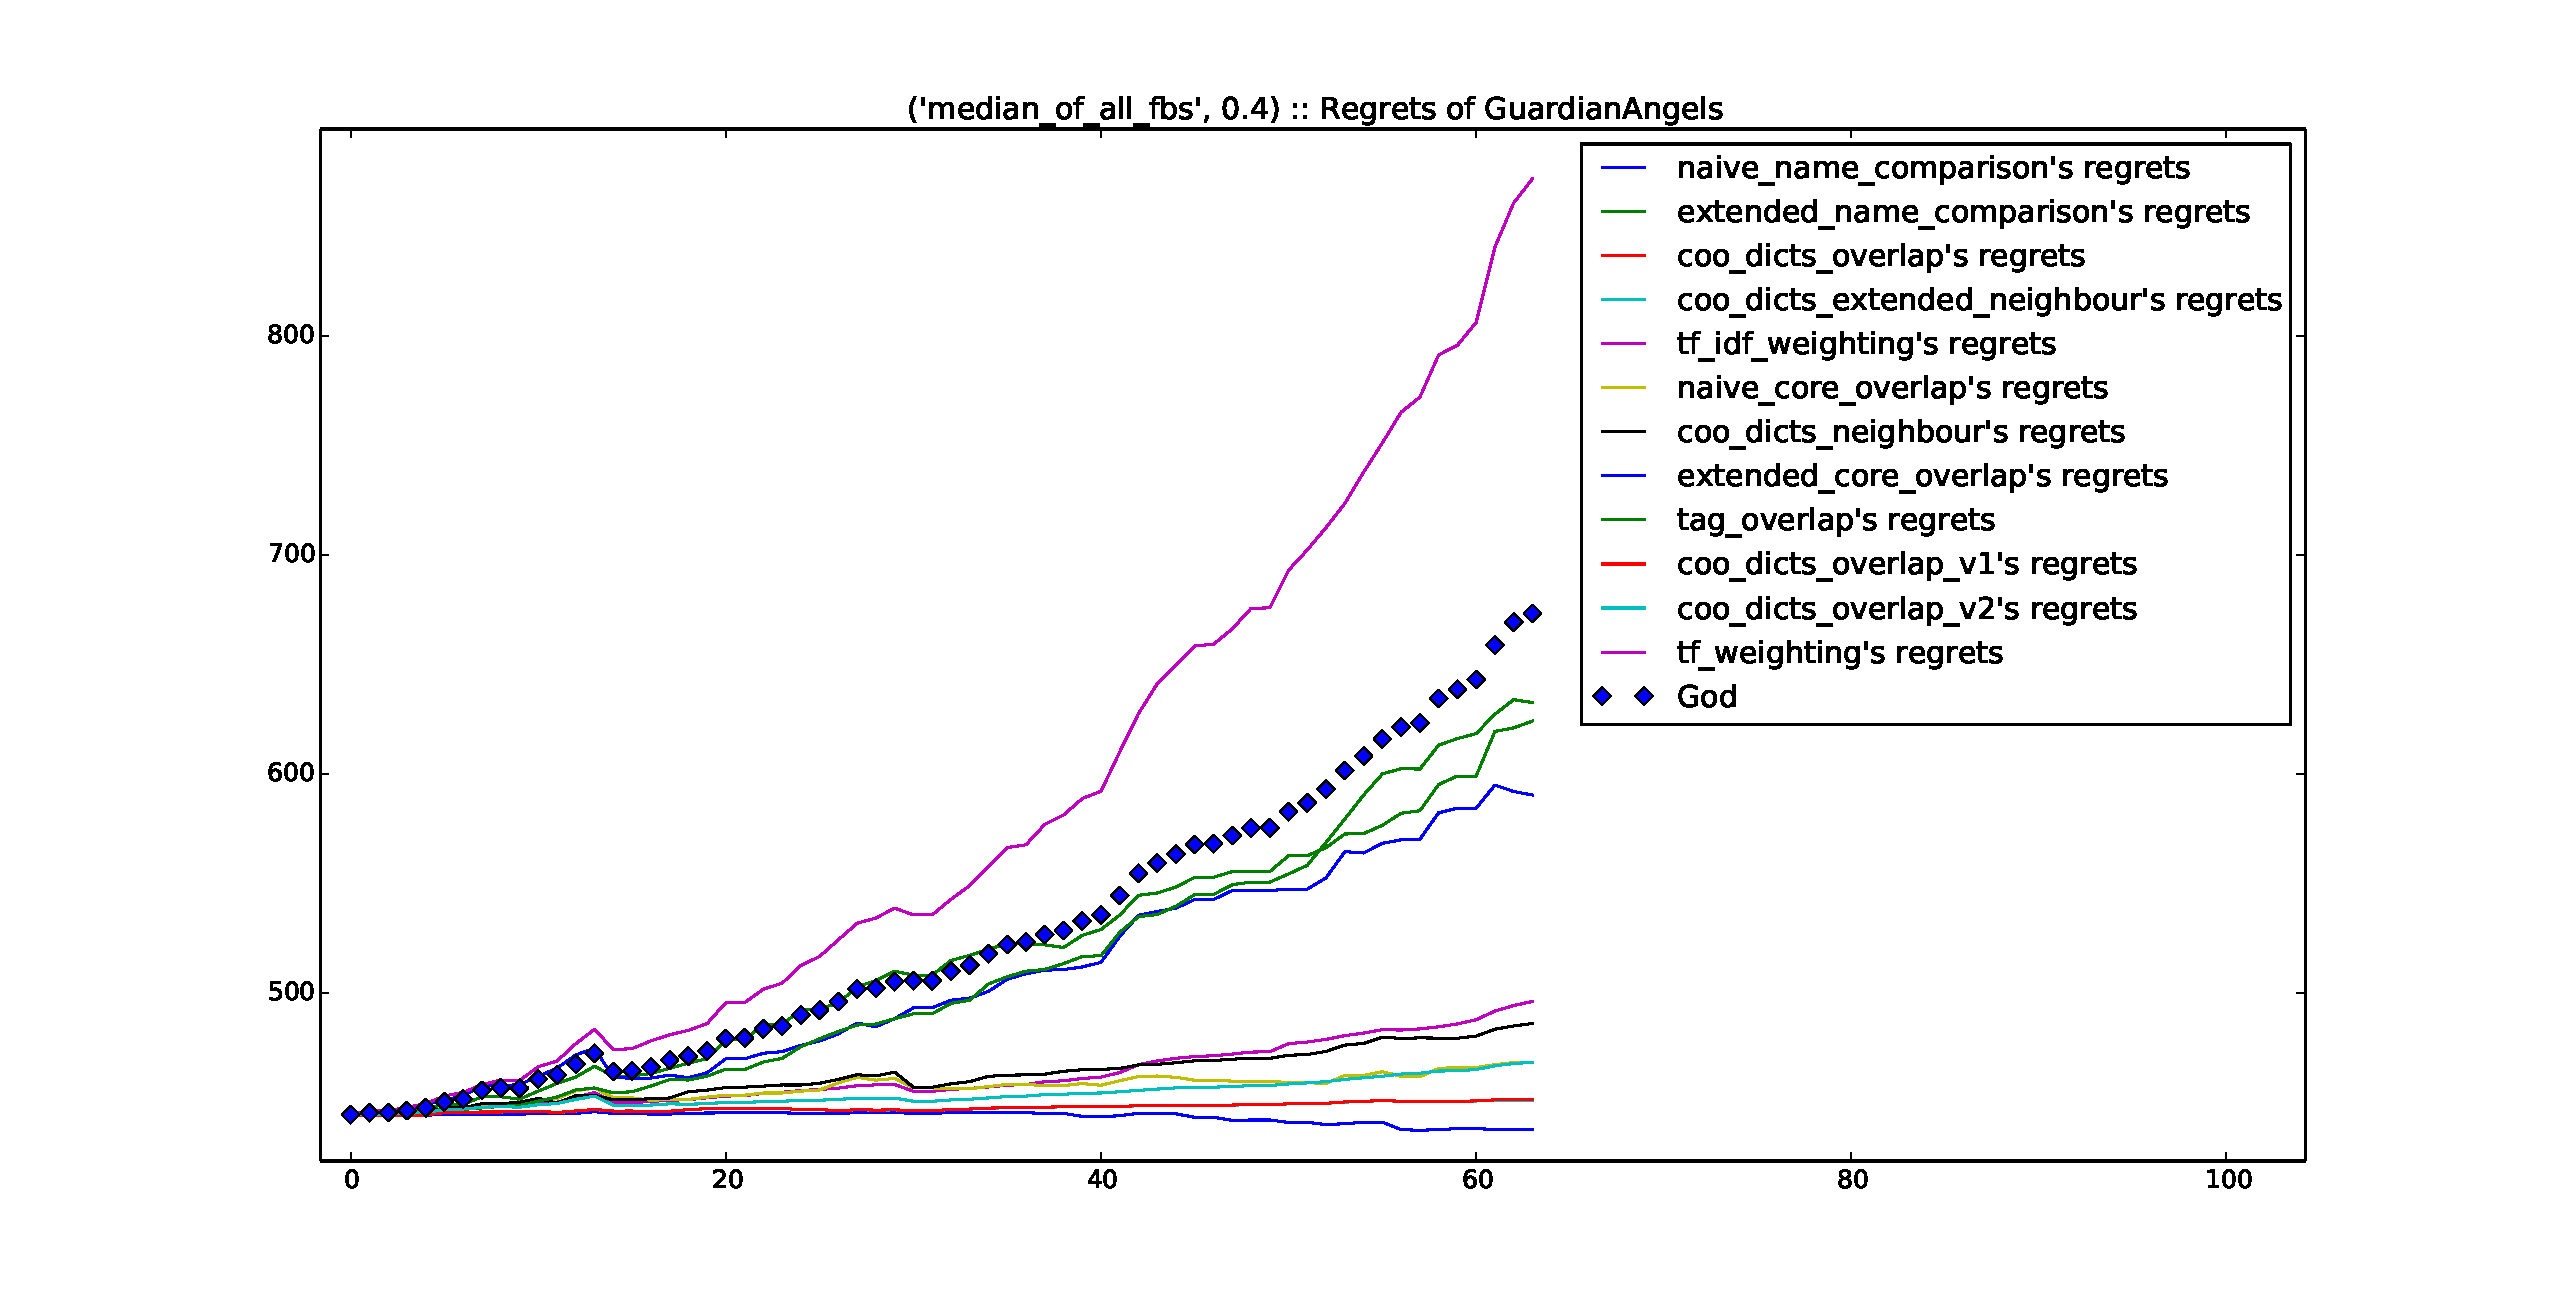
\includegraphics[width=\unitlength]{/home/pietro/Perceptum/code/starfish/similarity/SemanticSky/report_imgs/regrets.pdf}
    \hspace{-300pt} Figure \themyfigure: regrets on all links }%
  \end{picture}%
\endgroup%
\vspace{5pt}

Here one can see how for some algorithms (the least smart) regrets are increasing almost exponentially (in parallel with the increase of available permutations of clouds as the sky increases in size), whereas the regrets of some other algorithms are even decreasing. God seems to be driven a bit too high, not following the best ones, but the worse.\footnote{This probably being due to the fact that high regrets means high confidence in the wrong things: and high confidence means high impact on God's belief state.}

One can also notice that god's line is not the simple average of the other lines, but is a weighted average: it will be influenced (negatively) proportionally to the regrets of the angels. Ideally, an high-regrets angel should have low average weights, and thus influence less god's beliefs (and finally, god's regrets). The fact that this is not really happening here might mean that the low-regrets angels also have low average weights, which is in fact the case.

\paragraph{A few extra facts}:

The same test, with different parameters (learning speed $0.4$, update rule = \emph{average} of all feedback) yields comparable results (though perhaps a bit less nice):

\stepcounter{myfigure}
\def\svgwidth{500pt}
\begingroup%
  \makeatletter%
  \providecommand\color[2][]{%
    \errmessage{(Inkscape) Color is used for the text in Inkscape, but the package 'color.sty' is not loaded}%
    \renewcommand\color[2][]{}%
  }%
  \providecommand\transparent[1]{%
    \errmessage{(Inkscape) Transparency is used (non-zero) for the text in Inkscape, but the package 'transparent.sty' is not loaded}%
    \renewcommand\transparent[1]{}%
  }%
  \providecommand\rotatebox[2]{#2}%
  \ifx\svgwidth\undefined%
    \setlength{\unitlength}{1229.4bp}%
    \ifx\svgscale\undefined%
      \relax%
    \else%
      \setlength{\unitlength}{\unitlength * \real{\svgscale}}%
    \fi%
  \else%
    \setlength{\unitlength}{\svgwidth}%
  \fi%
  \global\let\svgwidth\undefined%
  \global\let\svgscale\undefined%
  \makeatother%
  \begin{picture}(1,0.50366032)%
    \put(-0.18,0){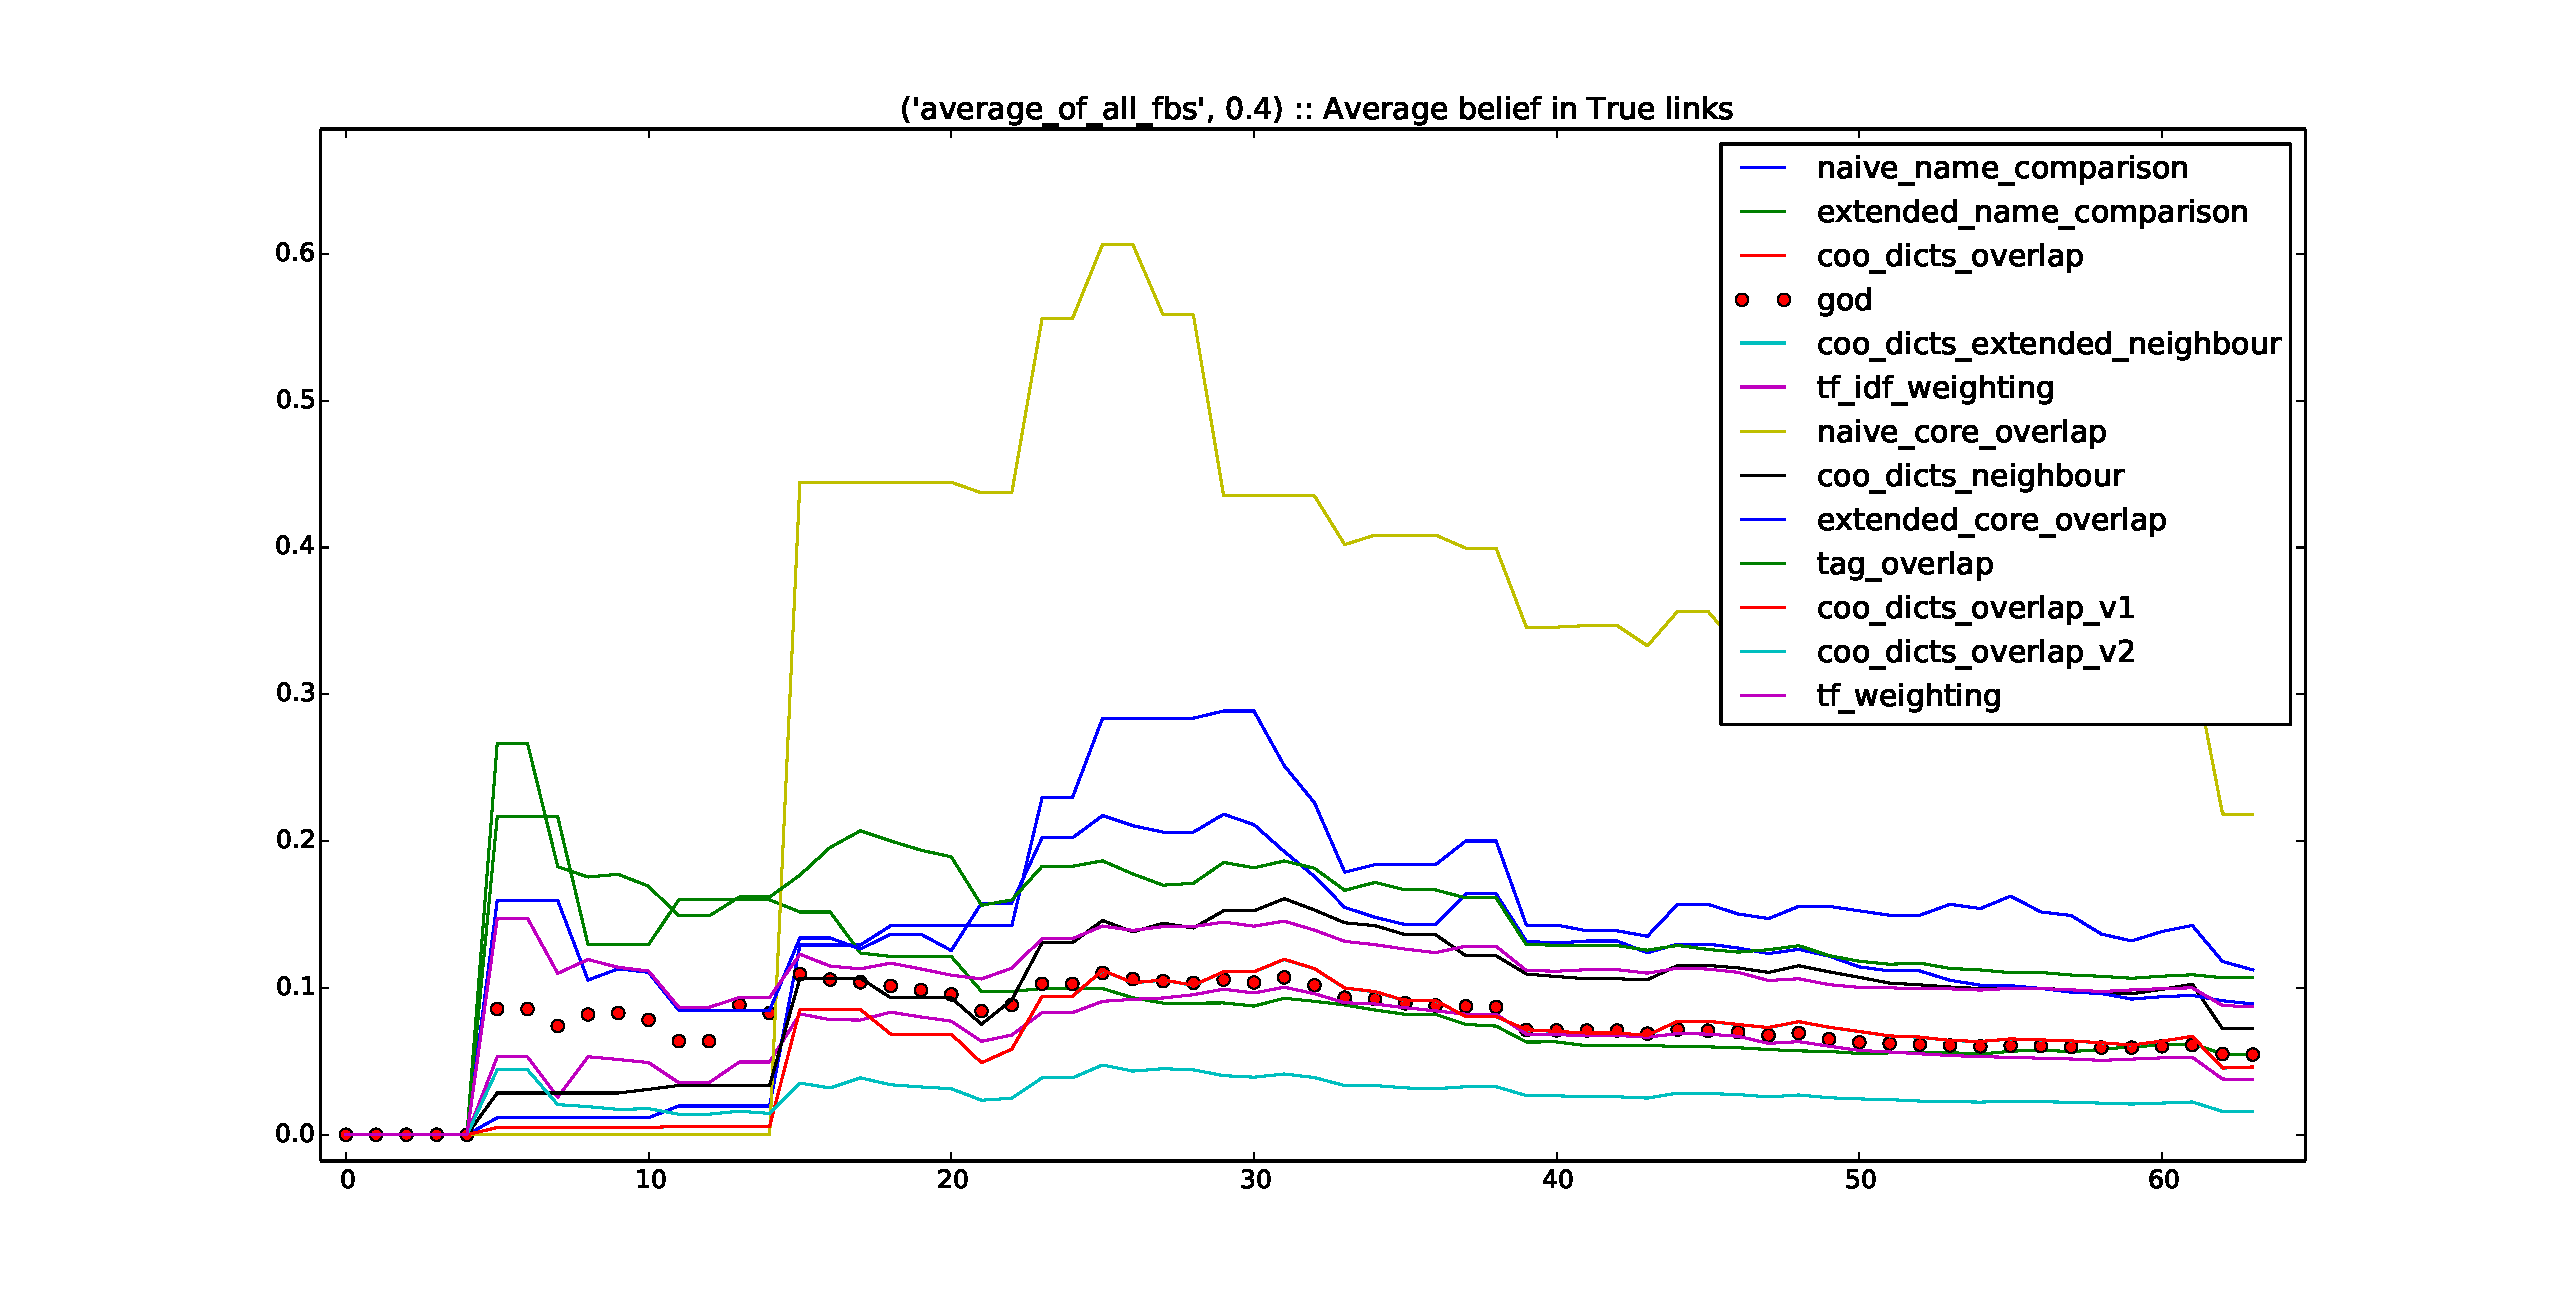
\includegraphics[width=\unitlength]{/home/pietro/Perceptum/code/starfish/similarity/SemanticSky/report_imgs/avgbelief_in_true_links.pdf}\hspace{-330pt} Figure \themyfigure : true links beliefs }%
  \end{picture}%
\endgroup%
\vspace{5pt}

\stepcounter{myfigure}
\def\svgwidth{500pt}
\begingroup%
  \makeatletter%
  \providecommand\color[2][]{%
    \errmessage{(Inkscape) Color is used for the text in Inkscape, but the package 'color.sty' is not loaded}%
    \renewcommand\color[2][]{}%
  }%
  \providecommand\transparent[1]{%
    \errmessage{(Inkscape) Transparency is used (non-zero) for the text in Inkscape, but the package 'transparent.sty' is not loaded}%
    \renewcommand\transparent[1]{}%
  }%
  \providecommand\rotatebox[2]{#2}%
  \ifx\svgwidth\undefined%
    \setlength{\unitlength}{1229.4bp}%
    \ifx\svgscale\undefined%
      \relax%
    \else%
      \setlength{\unitlength}{\unitlength * \real{\svgscale}}%
    \fi%
  \else%
    \setlength{\unitlength}{\svgwidth}%
  \fi%
  \global\let\svgwidth\undefined%
  \global\let\svgscale\undefined%
  \makeatother%
  \begin{picture}(1,0.50366032)%
    \put(-0.18,0){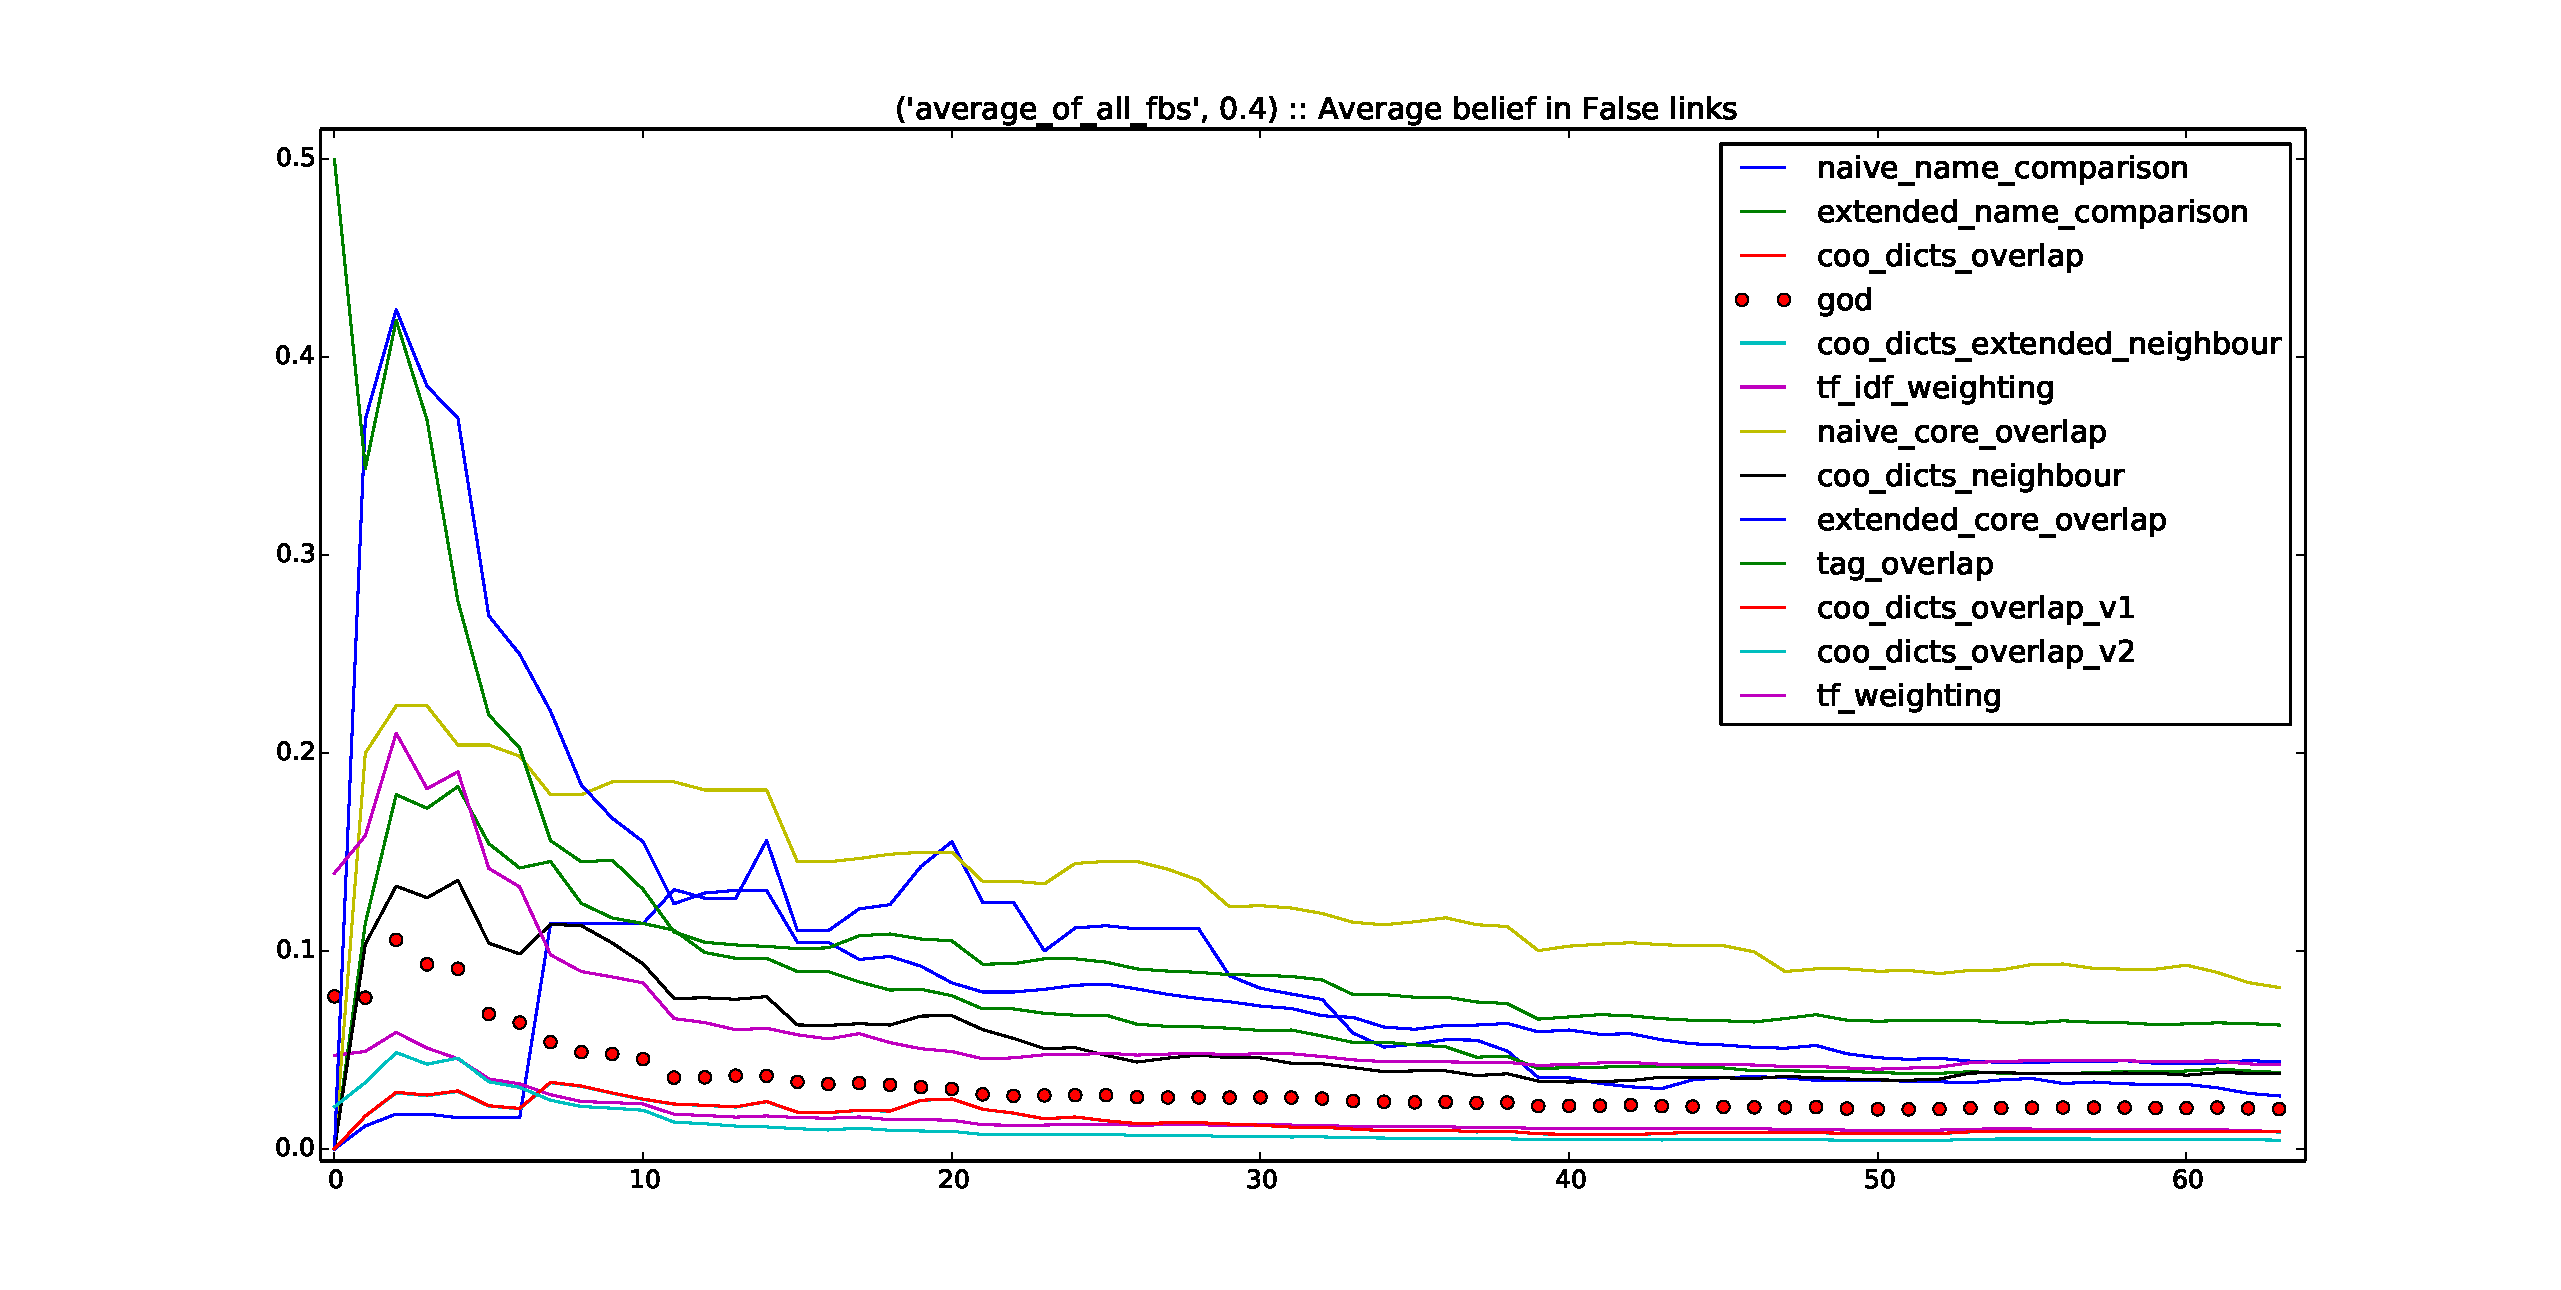
\includegraphics[width=\unitlength]{/home/pietro/Perceptum/code/starfish/similarity/SemanticSky/report_imgs/avgbelief_in_false_links.pdf}\hspace{-330pt} Figure \themyfigure : false links beliefs }%
  \end{picture}%
\endgroup%


\stepcounter{myfigure}
\def\svgwidth{550pt}
\begingroup%
  \makeatletter%
  \providecommand\color[2][]{%
    \errmessage{(Inkscape) Color is used for the text in Inkscape, but the package 'color.sty' is not loaded}%
    \renewcommand\color[2][]{}%
  }%
  \providecommand\transparent[1]{%
    \errmessage{(Inkscape) Transparency is used (non-zero) for the text in Inkscape, but the package 'transparent.sty' is not loaded}%
    \renewcommand\transparent[1]{}%
  }%
  \providecommand\rotatebox[2]{#2}%
  \ifx\svgwidth\undefined%
    \setlength{\unitlength}{1229.4bp}%
    \ifx\svgscale\undefined%
      \relax%
    \else%
      \setlength{\unitlength}{\unitlength * \real{\svgscale}}%
    \fi%
  \else%
    \setlength{\unitlength}{\svgwidth}%
  \fi%
  \global\let\svgwidth\undefined%
  \global\let\svgscale\undefined%
  \makeatother%
  \begin{picture}(1,0.50366032)%
    \put(-0.18,0){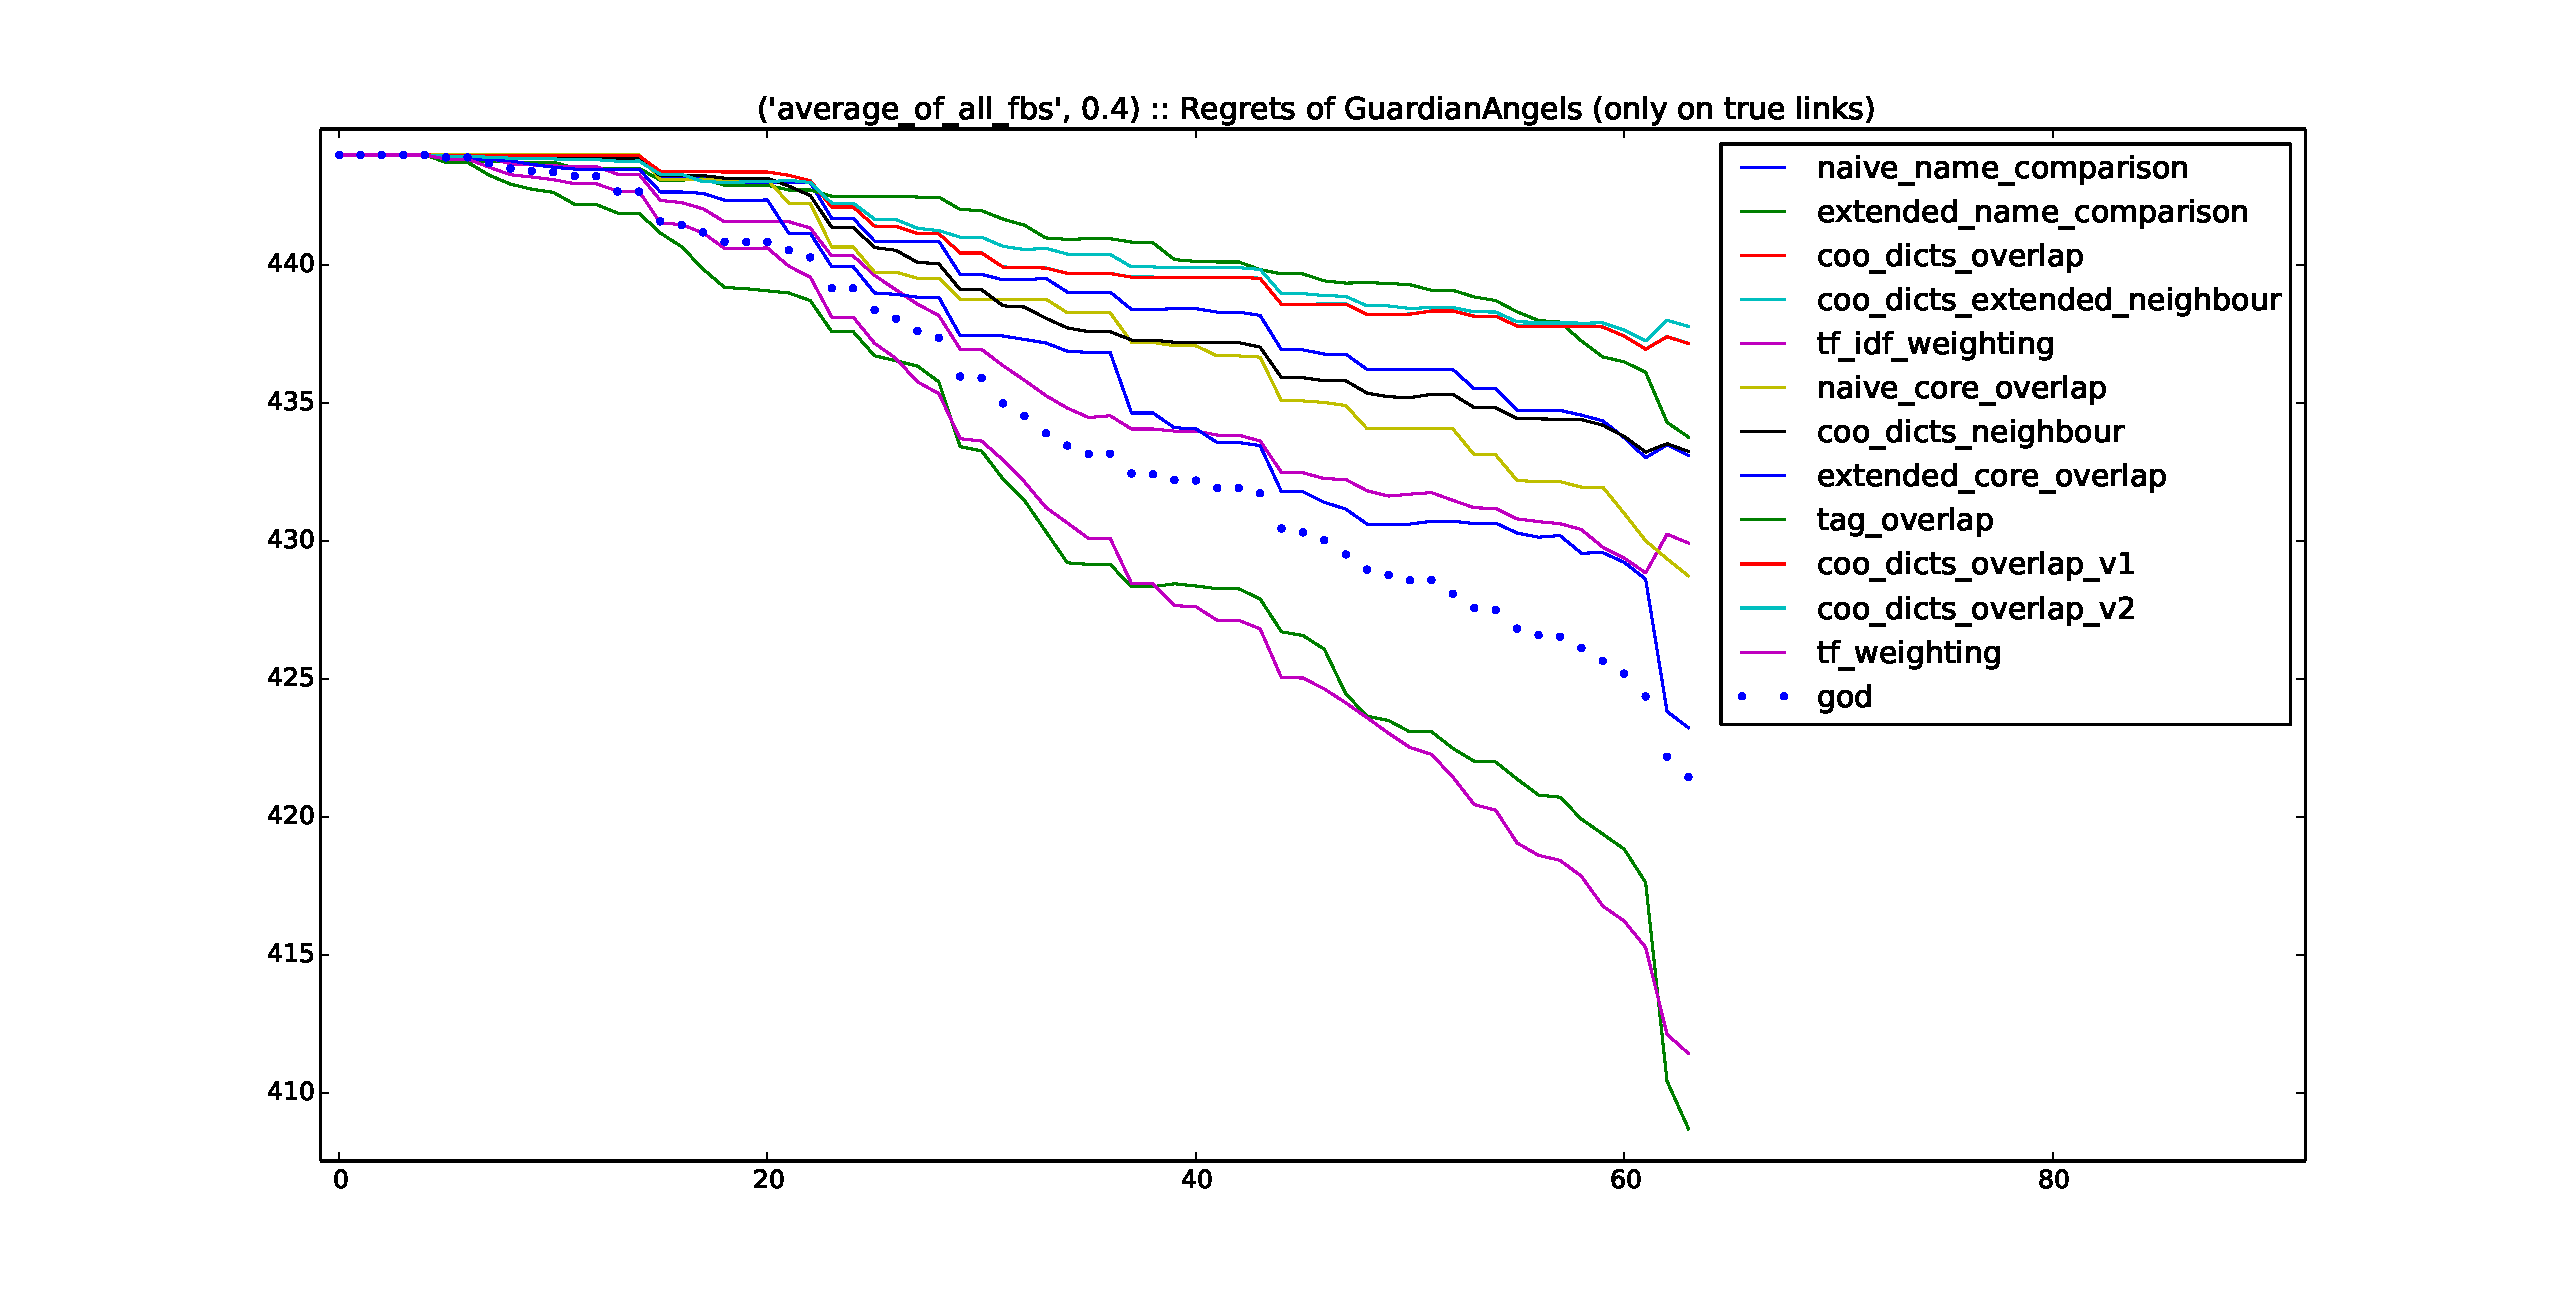
\includegraphics[width=\unitlength]{/home/pietro/Perceptum/code/starfish/similarity/SemanticSky/report_imgs/avgregrets_ontrue.pdf}\hspace{-355pt} Figure \themyfigure : regrets on true links }%
	
  \end{picture}%
\endgroup%

\stepcounter{myfigure}
\def\svgwidth{550pt}
\begingroup%
  \makeatletter%
  \providecommand\color[2][]{%
    \errmessage{(Inkscape) Color is used for the text in Inkscape, but the package 'color.sty' is not loaded}%
    \renewcommand\color[2][]{}%
  }%
  \providecommand\transparent[1]{%
    \errmessage{(Inkscape) Transparency is used (non-zero) for the text in Inkscape, but the package 'transparent.sty' is not loaded}%
    \renewcommand\transparent[1]{}%
  }%
  \providecommand\rotatebox[2]{#2}%
  \ifx\svgwidth\undefined%
    \setlength{\unitlength}{1229.4bp}%
    \ifx\svgscale\undefined%
      \relax%
    \else%
      \setlength{\unitlength}{\unitlength * \real{\svgscale}}%
    \fi%
  \else%
    \setlength{\unitlength}{\svgwidth}%
  \fi%
  \global\let\svgwidth\undefined%
  \global\let\svgscale\undefined%
  \makeatother%
  \begin{picture}(1,0.50366032)%
    \put(-0.18,0){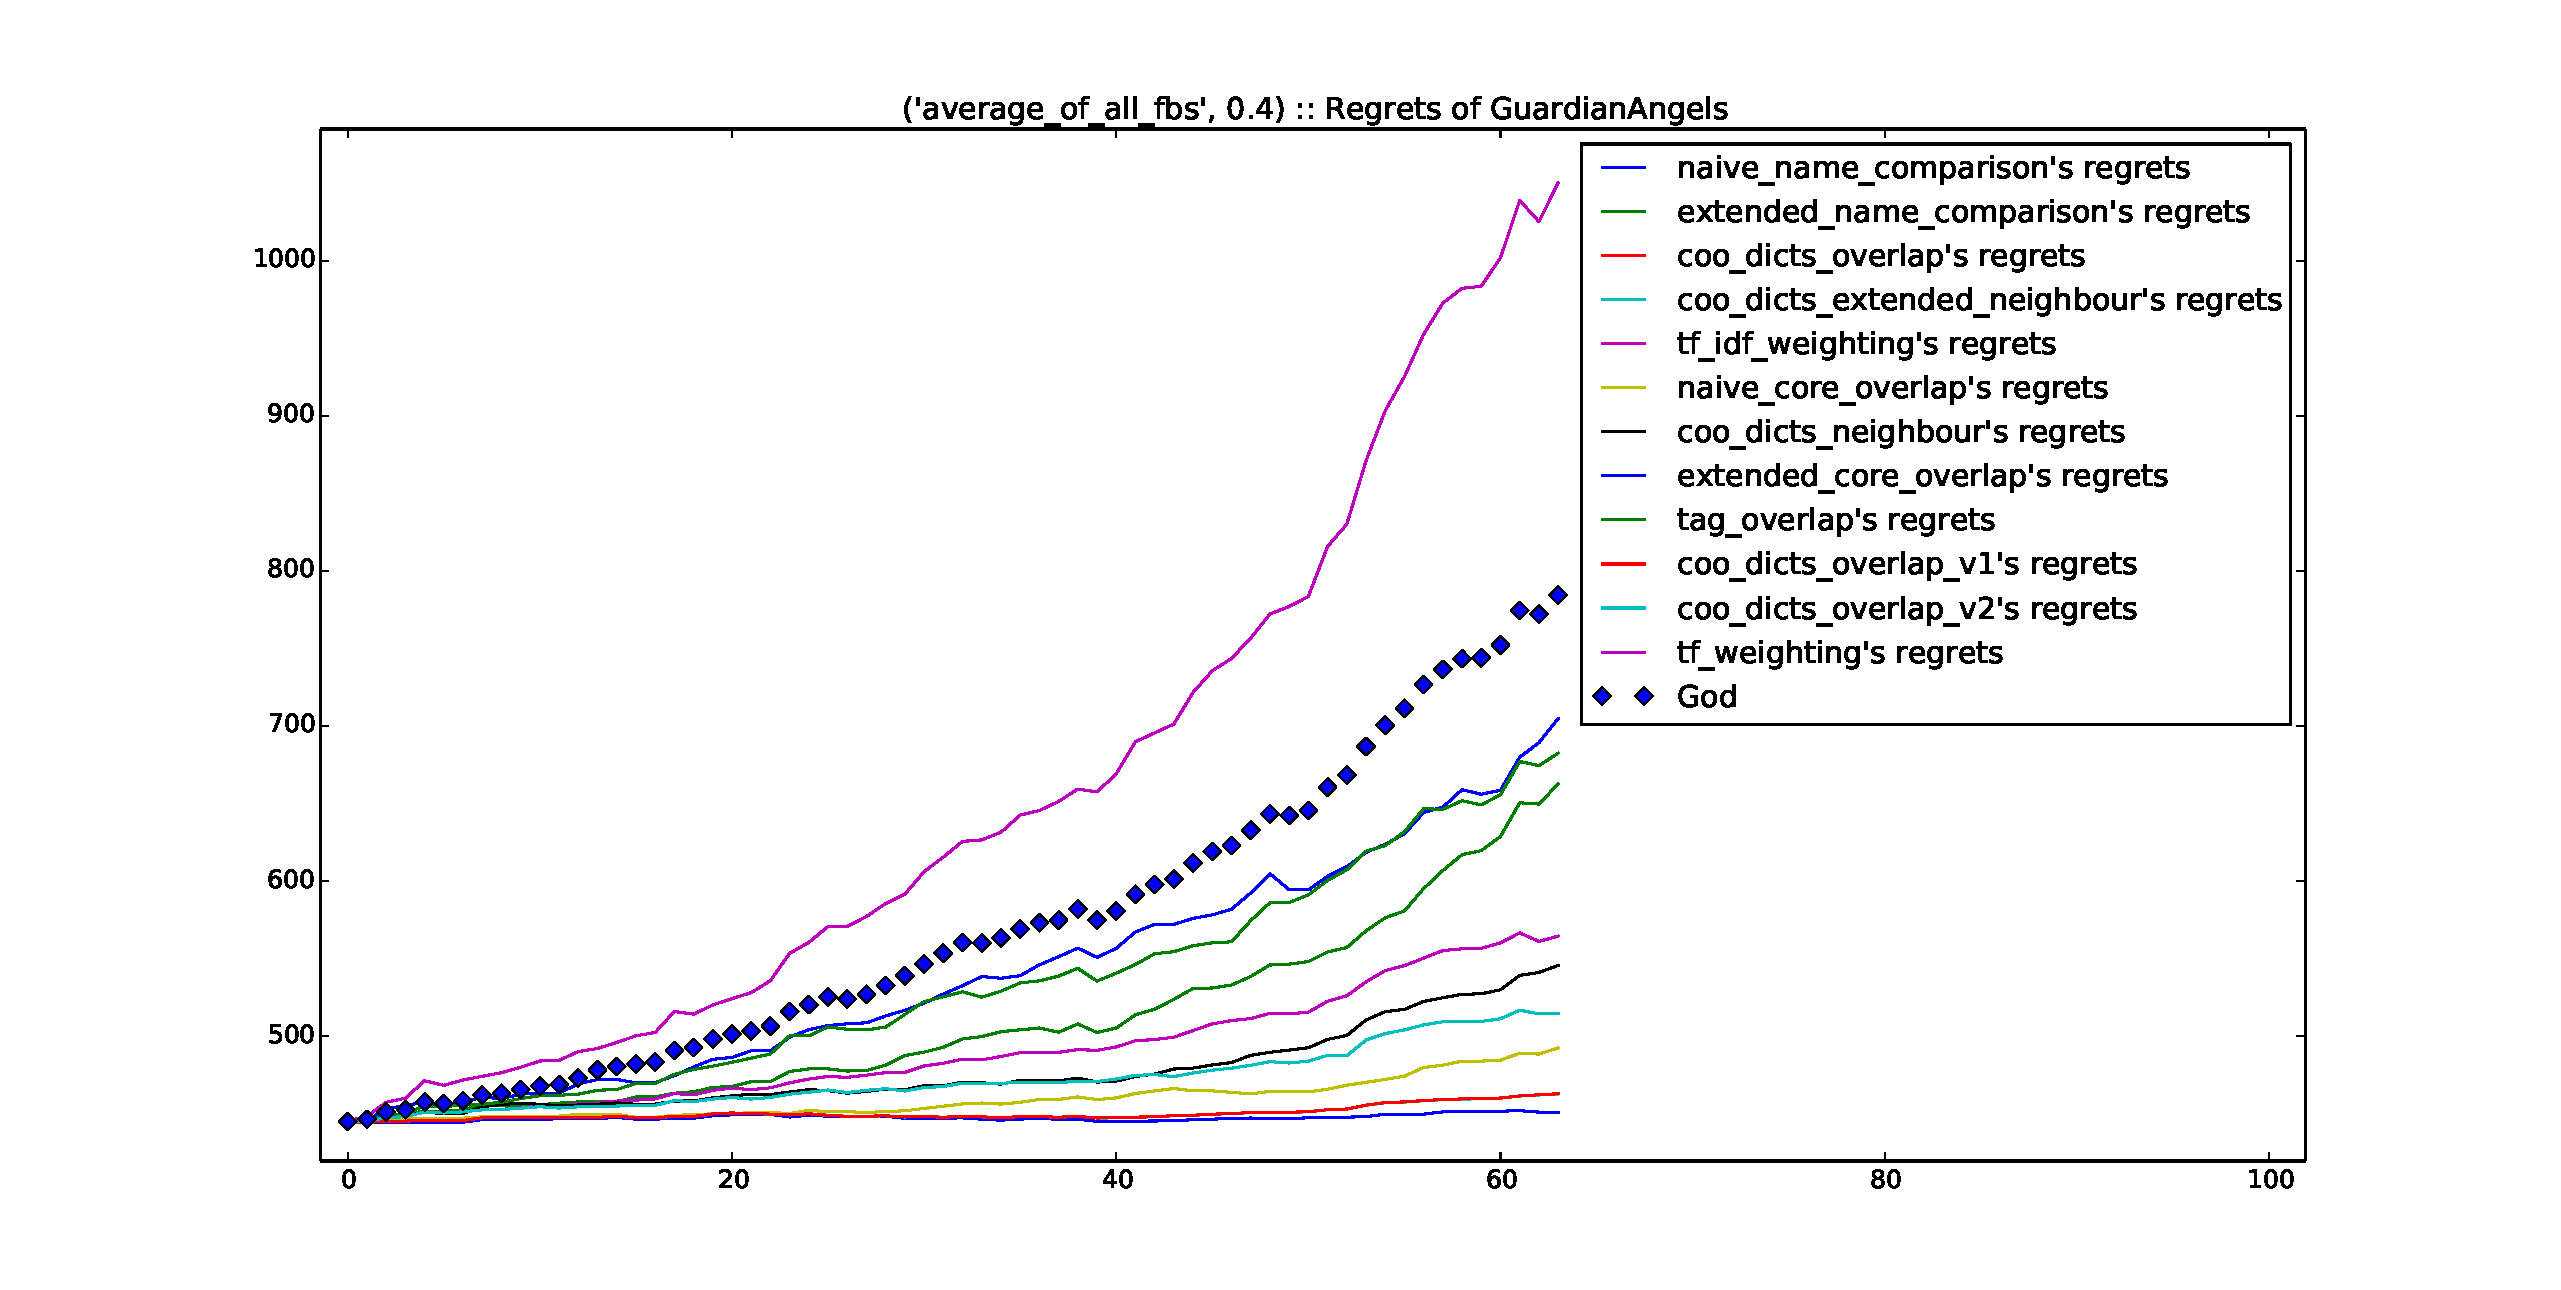
\includegraphics[width=\unitlength]{/home/pietro/Perceptum/code/starfish/similarity/SemanticSky/report_imgs/avgregrets.pdf}\hspace{-355pt} Figure \themyfigure : regrets on all links }%
	
  \end{picture}%
\endgroup%


\subsubsection{Analysing the test output.}

Summing up, tests of this kind were ran with the following parameters:

\begin{itemize}
\item Median, learning rates 0.2, 0.4(2), 0.5, 0.8, 1.

\item Average, learning rates 0.4(2), 0.8, 1.

\item Step by step average, learning rate 0.2, 0.8.

\item Median and average, learning rate 0.2, punish = True\footnote{This means that feedback was given not on known truths but also on unknown pairs (which, we remind, are assumed to have similarity $0$'). More on this in the appendix.}.
\end{itemize}

From these tests clearly emerged that regret on true links (figures 3 and 6) stably decreased, but average belief in true links stays as low as 0.05.

Also, since clouds were added in batches of 5 or 6, and regret on true links depends on the amount of true links available given the current cloud set, it's unclear whether the (final) regrets would have been lower, had the weights permanently all been set to 1.

This doubt is easily dispelled, and the answer follows in a graph. 


\stepcounter{myfigure}
\def\svgwidth{360pt}
\begingroup%
  \makeatletter%
  \providecommand\color[2][]{%
    \errmessage{(Inkscape) Color is used for the text in Inkscape, but the package 'color.sty' is not loaded}%
    \renewcommand\color[2][]{}%
  }%
  \providecommand\transparent[1]{%
    \errmessage{(Inkscape) Transparency is used (non-zero) for the text in Inkscape, but the package 'transparent.sty' is not loaded}%
    \renewcommand\transparent[1]{}%
  }%
  \providecommand\rotatebox[2]{#2}%
  \ifx\svgwidth\undefined%
    \setlength{\unitlength}{1229.4bp}%
    \ifx\svgscale\undefined%
      \relax%
    \else%
      \setlength{\unitlength}{\unitlength * \real{\svgscale}}%
    \fi%
  \else%
    \setlength{\unitlength}{\svgwidth}%
  \fi%
  \global\let\svgwidth\undefined%
  \global\let\svgscale\undefined%
  \makeatother%
  \begin{picture}(1,0.50366032)%
    \put(-0.08,0){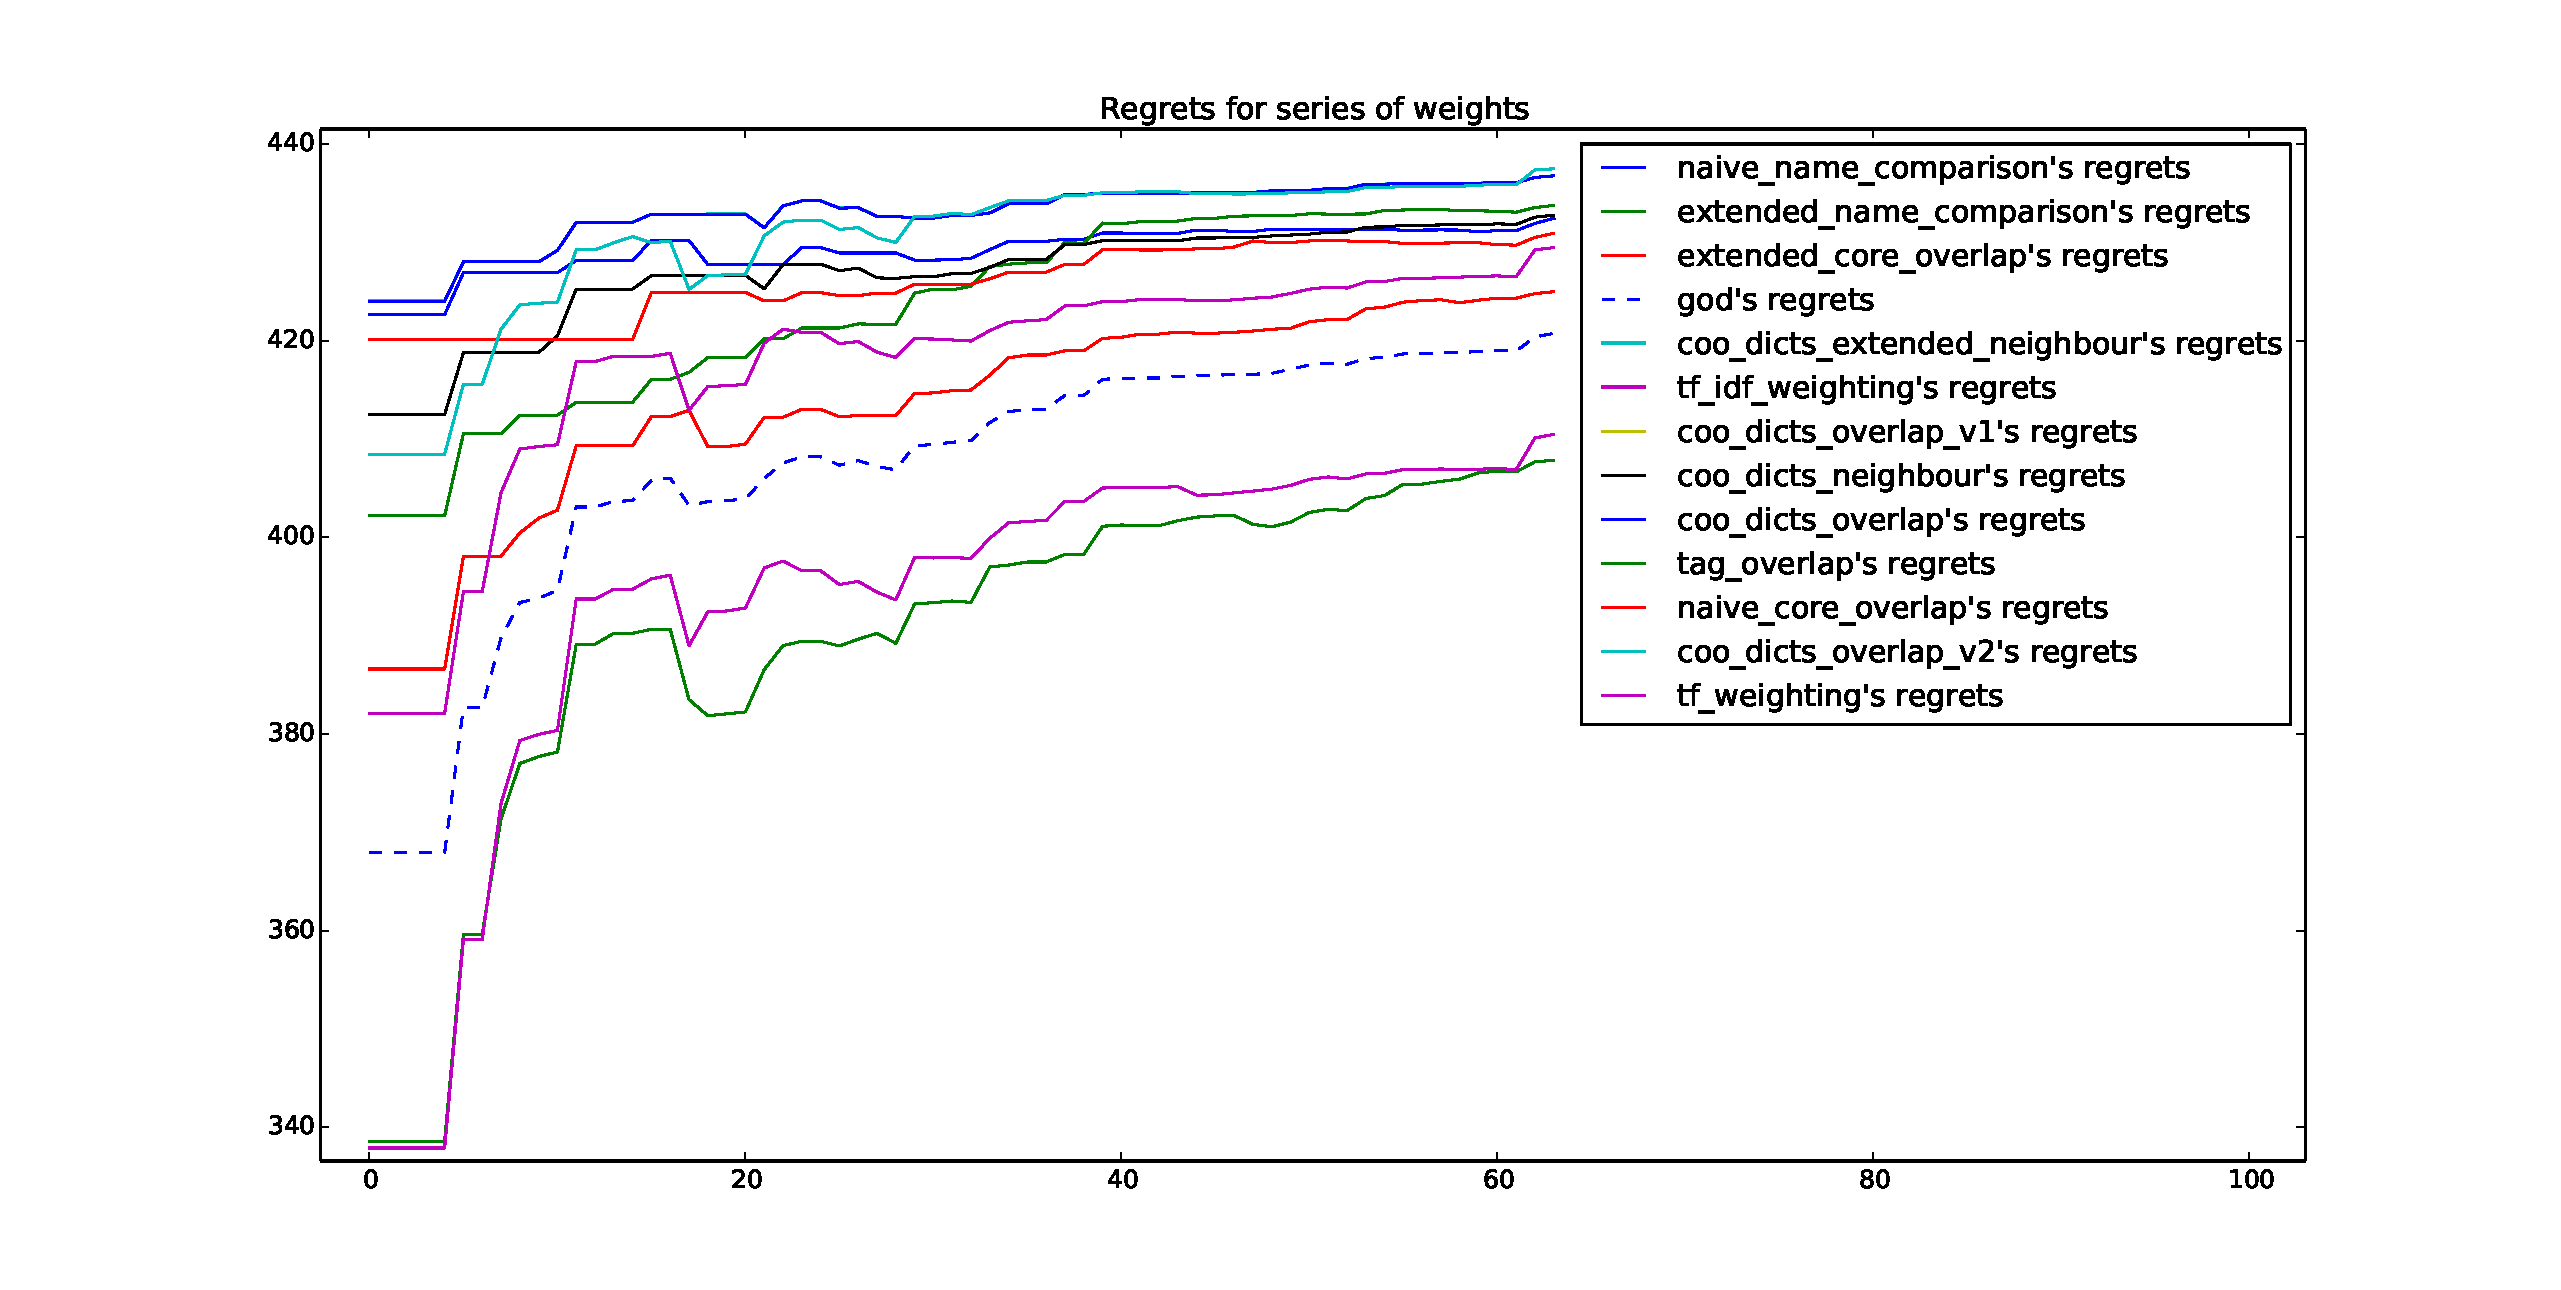
\includegraphics[width=\unitlength]{/home/pietro/Perceptum/code/starfish/similarity/SemanticSky/report_imgs/regrets_for_series_of_weights_ontrue.pdf}\hspace{-280pt} Figure \themyfigure : regrets on true links : absolute }%
	
  \end{picture}%
\endgroup%
\vspace{5pt}
This graph represents what happens to a belief set whose weights have been all set to 1 (their initial value), if we assign to it the weights as they have come out of the test we just described. Each step on the $x$ axis then represents the non-cumulative regret at that moment, and depends solely on the weights we have assigned to the system at that step.

As the weights evolve (via feedback) from their initial value to their final one, we can see that the regrets for true links is actually increasing.

Even though, if we don't just look at true links, regrets are falling:


\stepcounter{myfigure}
\def\svgwidth{360pt}
\begingroup%
  \makeatletter%
  \providecommand\color[2][]{%
    \errmessage{(Inkscape) Color is used for the text in Inkscape, but the package 'color.sty' is not loaded}%
    \renewcommand\color[2][]{}%
  }%
  \providecommand\transparent[1]{%
    \errmessage{(Inkscape) Transparency is used (non-zero) for the text in Inkscape, but the package 'transparent.sty' is not loaded}%
    \renewcommand\transparent[1]{}%
  }%
  \providecommand\rotatebox[2]{#2}%
  \ifx\svgwidth\undefined%
    \setlength{\unitlength}{1229.4bp}%
    \ifx\svgscale\undefined%
      \relax%
    \else%
      \setlength{\unitlength}{\unitlength * \real{\svgscale}}%
    \fi%
  \else%
    \setlength{\unitlength}{\svgwidth}%
  \fi%
  \global\let\svgwidth\undefined%
  \global\let\svgscale\undefined%
  \makeatother%
  \begin{picture}(1,0.50366032)%
    \put(-0.08,0){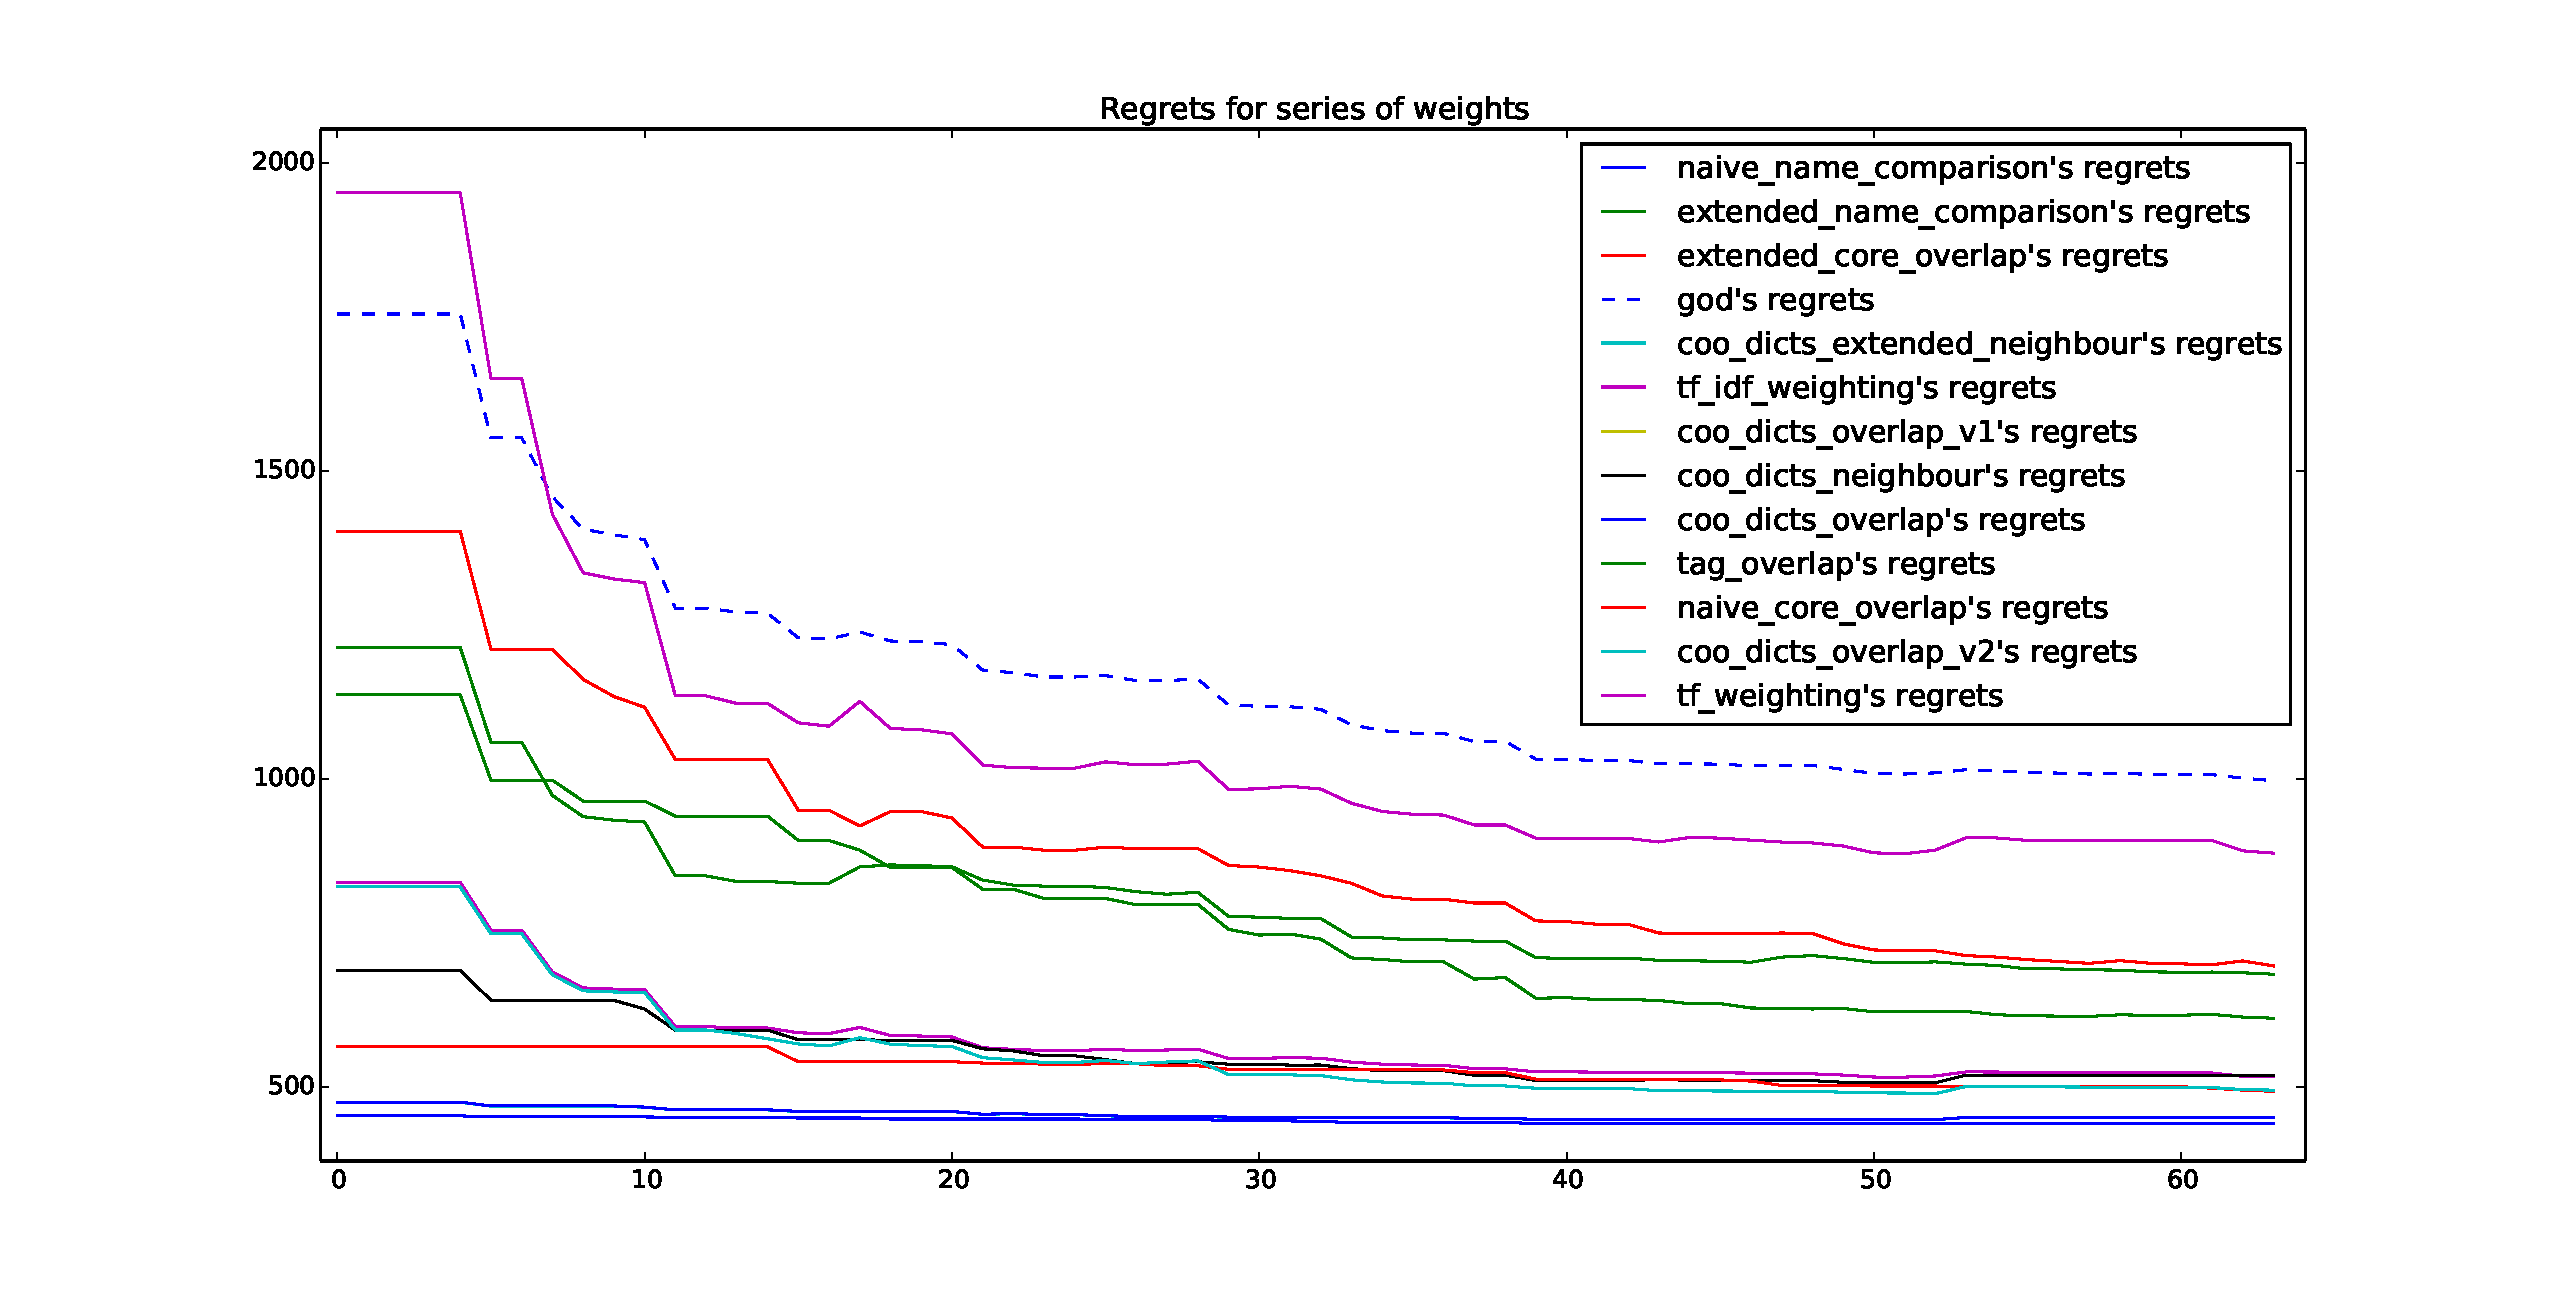
\includegraphics[width=\unitlength]{/home/pietro/Perceptum/code/starfish/similarity/SemanticSky/report_imgs/regrets_for_series_of_weights.pdf}\hspace{-280pt} Figure \themyfigure : regrets on all links : absolute }%
	
  \end{picture}%
\endgroup%
\vspace{5pt}

So, at an absolute level, it seems that the system is learning the golden rule `if the 99\% of the times the right answer is ``no'', then I better just say no every time.' To face this situation, it seemed natural to go for some ways of countering sample bias, which is nonetheless out of the scope of the present report.\footnote{There is more on it in the Appendix, however.}

\subsection{What comes next.}

$\bullet \quad$ During the development of SemanticSky we had several intuitions of possible things to do, or possible alternative ways of doing things we were already doing. For example, when giving feedback, the standard way to go is to give a feedback closer to 1 the closer my evaluation of x is to the evaluation of whoever I am giving feedback to. A different option however is to give straight what should be, in my opinion, the evaluation for that item. While training, this is basically equivalent to having the knower give a 0-1 feedback or a continuum between 0 and 1 (closer to 1 for high confidence correct answers or low confidence false answers, and vice versa). We have run a couple of tests with this alternative algorithm, but due to lack of time we could not double check them and we have no definitive conclusions to draw.

This and a number of options can and need be discussed. Probably, a bit more conceptual analysis ahead of a `now sit down and experiment' is preferable, in this case, being there so many parameters at stake whose interplay is in most cases too complex to have a clear balance.

$\bullet \quad$ Closely related to the previous point, the issue on whether to give feedback on false negatives is still open. The main way to find a quick answer to this problem is, to my mind, to run a bunch of test flipping the switch on and off, and see what happens. This has not been done yet due to lack of machine time.

$\bullet \quad$ Another thing that is missing is some sort of benchmarking: we had some ideas about trying to SemanticSky our way through the immense Wikipedia API or LastFm, IGN, or one of the many databases available.

To extend the framework to deal with that kind of clouds is quite straightforward. The main obstacle, for the moment, seems computational in nature: if we choose to punish false negatives (and the answer to `should we do it' is still open), an evaluation on Starfish takes more than two or three days on my laptop. I wonder how many weeks would it take with (a subsection of) Wikipedia. But, given time and a machine one does not need to Skype his girlfriend, this is clearly something we want to do.

$\bullet \quad$ For the moment we did not have time to generalize (codewise) the cloud-formation process. Some programming effort should be taken into doing that in a wise way.

\subsection{Generalization.}

How general is SemanticSky, or how long would it take to make it (more) general?

To our mind, SemanticSky is quite general already. What is Starfish-specific, for the moment, is the cloud-formation process (that relies quite heavily on the information we have from Starfish) and in the Angels, that are built to use exactly these features.

Namely, the database the system has been designed to work with contains data which is partially tagged: each item has a `title' field, an `author', and so on: what if it had not?
There are many ways to go with untagged data (which would turn SemanticSky) closer to the unsupervised side of the semi-supervised class of approaches: we could either have some algorithms to pre-classify the documents or parts of them (for example to extract tags, or titles, to recognize authorship or inter-document relations) or we could have very simple clouds with only a `text' entry, and our angels will have to be smart and diverse enough to work on that sort of data without any more tagged input.

Technically, all the work done by clouds could as well be done by Angels alone. The main idea behind clouds was to do beforehand something that angels would have needed to do themselves many times, such as tokenizing the text down to words, stemming, and extracting the tags that came along with the items. But there is no principled reason (if not maybe some computational considerations) for which we should keep the two things separated: we might as well decide to abandon the whole cloud principle and have the algorithms evaluate over the raw items, whatever they are, provided they come with the same toplevel data structure (otherwise, also Angels would need to be modified each time).

Personally, I think the cloud layer is not a bad thing and should be kept, mainly because it allows to standardise the input we receive to a more intuitive form, which all angels (regardless of what kind of data they were built to evaluate on) can accept without crashing.

Regarding the way Angels can be generalized there is probably little to say: as specific entities they probably can't. What can be generalized is the framework, and probably angels will need to be written depending on the form of the items we are trying to evaluate upon. We might for example build a SemanticSky that recognizes similarities between songs. Then clouds would store some metadata, if available, or extract some features which we deem relevant such as bpm, number of layers, compression level, noise, and more. But, most likely, a tf/idf weighting algorithm will do little if this is all we have, and output 0 all the time.

Of course, we could build an algorithm that just evaluates the similarity of two clouds at a higher level, but that would be a SemanticSky itself, and is not really what we want. Generalization of algorithms, in other words, is out of the scope here. What we had in mind is to make a general framework, but the supervised part of building the specific algorithms able to crunch the data we give them is not (as far as I can see) going to disappear soon.

This is, if you want, the lower bound of the current SemanticSky-paradigm.






\part{Appendices.}
\section{Punishing.}

The decision to only give feedback on known truths (thus not penalising false positives [what I say is, but is not]) can be questioned. Also, no (negative) feedback is given on false negatives, and this is even more questionable.

In short, feedback is given to all and only those angels which have a non-zero opinion about a link which we know to be true. Angels which spot similarities where we know there are none (false positives), or angels who don't spot similarities where we know there are (false negatives), are not punished for this, for two different reasons.

\paragraph{Reasons for not punishing for false negatives:} the main one I can see is that we chose to interpret the decision of the angels not as opinions about the relatedness of items, but about confidence ratios about such relation.

The difference is subtle but important: if an algorithm returns 0.5 when fed with two clouds, you can interpret that output in at least two ways:

\begin{itemize}
\item[\textbf{relatedness}] ``I believe these two items to be 0.5 related / they have 50\% in common / they resemble to each other half of how they would if they were exactly equal.''
\item[\textbf{confidence}] ``I am not entirely sure, but 5 out of 10 these two items are related / I am 50\% confident in the relatedness of these two clouds.''
\end{itemize}

The most relevant outcome of this distinction is that on the relatedness reading, a 0/10 rating means `my opinion is that these two items are not related', whereas on the confidence rating that would be a milder `I have no reason to believe they are related, but I just don't know'.

Given that the algorithms we used were relatively naive and relied, as explained in the appropriate section of this report, on a (very) restricted subset of the available evidence, it seemed obvious to use the `confidence' interpretation of their opinions instead of the other one: they have to be humble about their judgements. Their perceptual field is so narrow that an output of 0 is hardly interpreted as a negative relatedness judgement, but rather as a `here I can't see anything' statement.

As a consequence of these considerations, we chose not to punish the angels for their false negatives: if they can't see anything, it's not their fault and there's nothing they can do about it: it's not by lowering their (relative) trustworthiness that we will improve the situation.

\paragraph{Reasons for not punishing for false positives:}

First of all, the Knower's belief set is assumed to be `all there is to know', literally, but in a dynamic frame such as Starfish's one, we want to always keep the discussion going. When the state of the discussion (the state of the art, if you wish) is not yet settled, when there is no agreement or just too little opinions to have a definitive decision, then the rationale of `all there is to know' becomes questionable.

But most crucially, what matters for the purpose of classification is not the unrealistic target of all and only true items being detected as such (zero false negatives and false positives), but that the gap in the confidences is wide enough to allow for a nice separation of them from the false ones (via ranking, for suggestions, or by thresholding, for selection of links.)

And, as it comes out, the angels are already somewhat good to do this as they are. The average confidence in true links against false links is, as it has been previously shown, clearly in advantage of true links. So, instead of punishing an angel's relative trustworthiness regarding some link type because of its (many) errors in which he nonetheless has very low confidence, thereby lowering the future impact of his (few) right clues in which he has a higher confidence, we could just not give bad feedback on the low-confidence errors.

Clearly if an angel had high confidence on some or many errors, the situation would need more accurate consideration, and it might even be worth considering some thresholded triggering of feedback based precisely on a trustworthiness / confidence function, so that we give feedback on items only when the angel is trustworthy enough in his own suggestion.


\paragraph{A backing experiment.}

As a partial proof of the usefulness/correctness of this stance, we ran a test in which we set the punish flag to True, thus giving feedback to false positives (to give feedback on false negatives is currently just not possible in the framework, but it will in the future). Graphs of the outcome follows, and are rather self-explanatory. Update rule: median, learning speed 0.2. 

\stepcounter{myfigure}
\def\svgwidth{500pt}
\begingroup%
  \makeatletter%
  \providecommand\color[2][]{%
    \errmessage{(Inkscape) Color is used for the text in Inkscape, but the package 'color.sty' is not loaded}%
    \renewcommand\color[2][]{}%
  }%
  \providecommand\transparent[1]{%
    \errmessage{(Inkscape) Transparency is used (non-zero) for the text in Inkscape, but the package 'transparent.sty' is not loaded}%
    \renewcommand\transparent[1]{}%
  }%
  \providecommand\rotatebox[2]{#2}%
  \ifx\svgwidth\undefined%
    \setlength{\unitlength}{1229.4bp}%
    \ifx\svgscale\undefined%
      \relax%
    \else%
      \setlength{\unitlength}{\unitlength * \real{\svgscale}}%
    \fi%
  \else%
    \setlength{\unitlength}{\svgwidth}%
  \fi%
  \global\let\svgwidth\undefined%
  \global\let\svgscale\undefined%
  \makeatother%
  \begin{picture}(1,0.50366032)%
    \put(-0.18,0){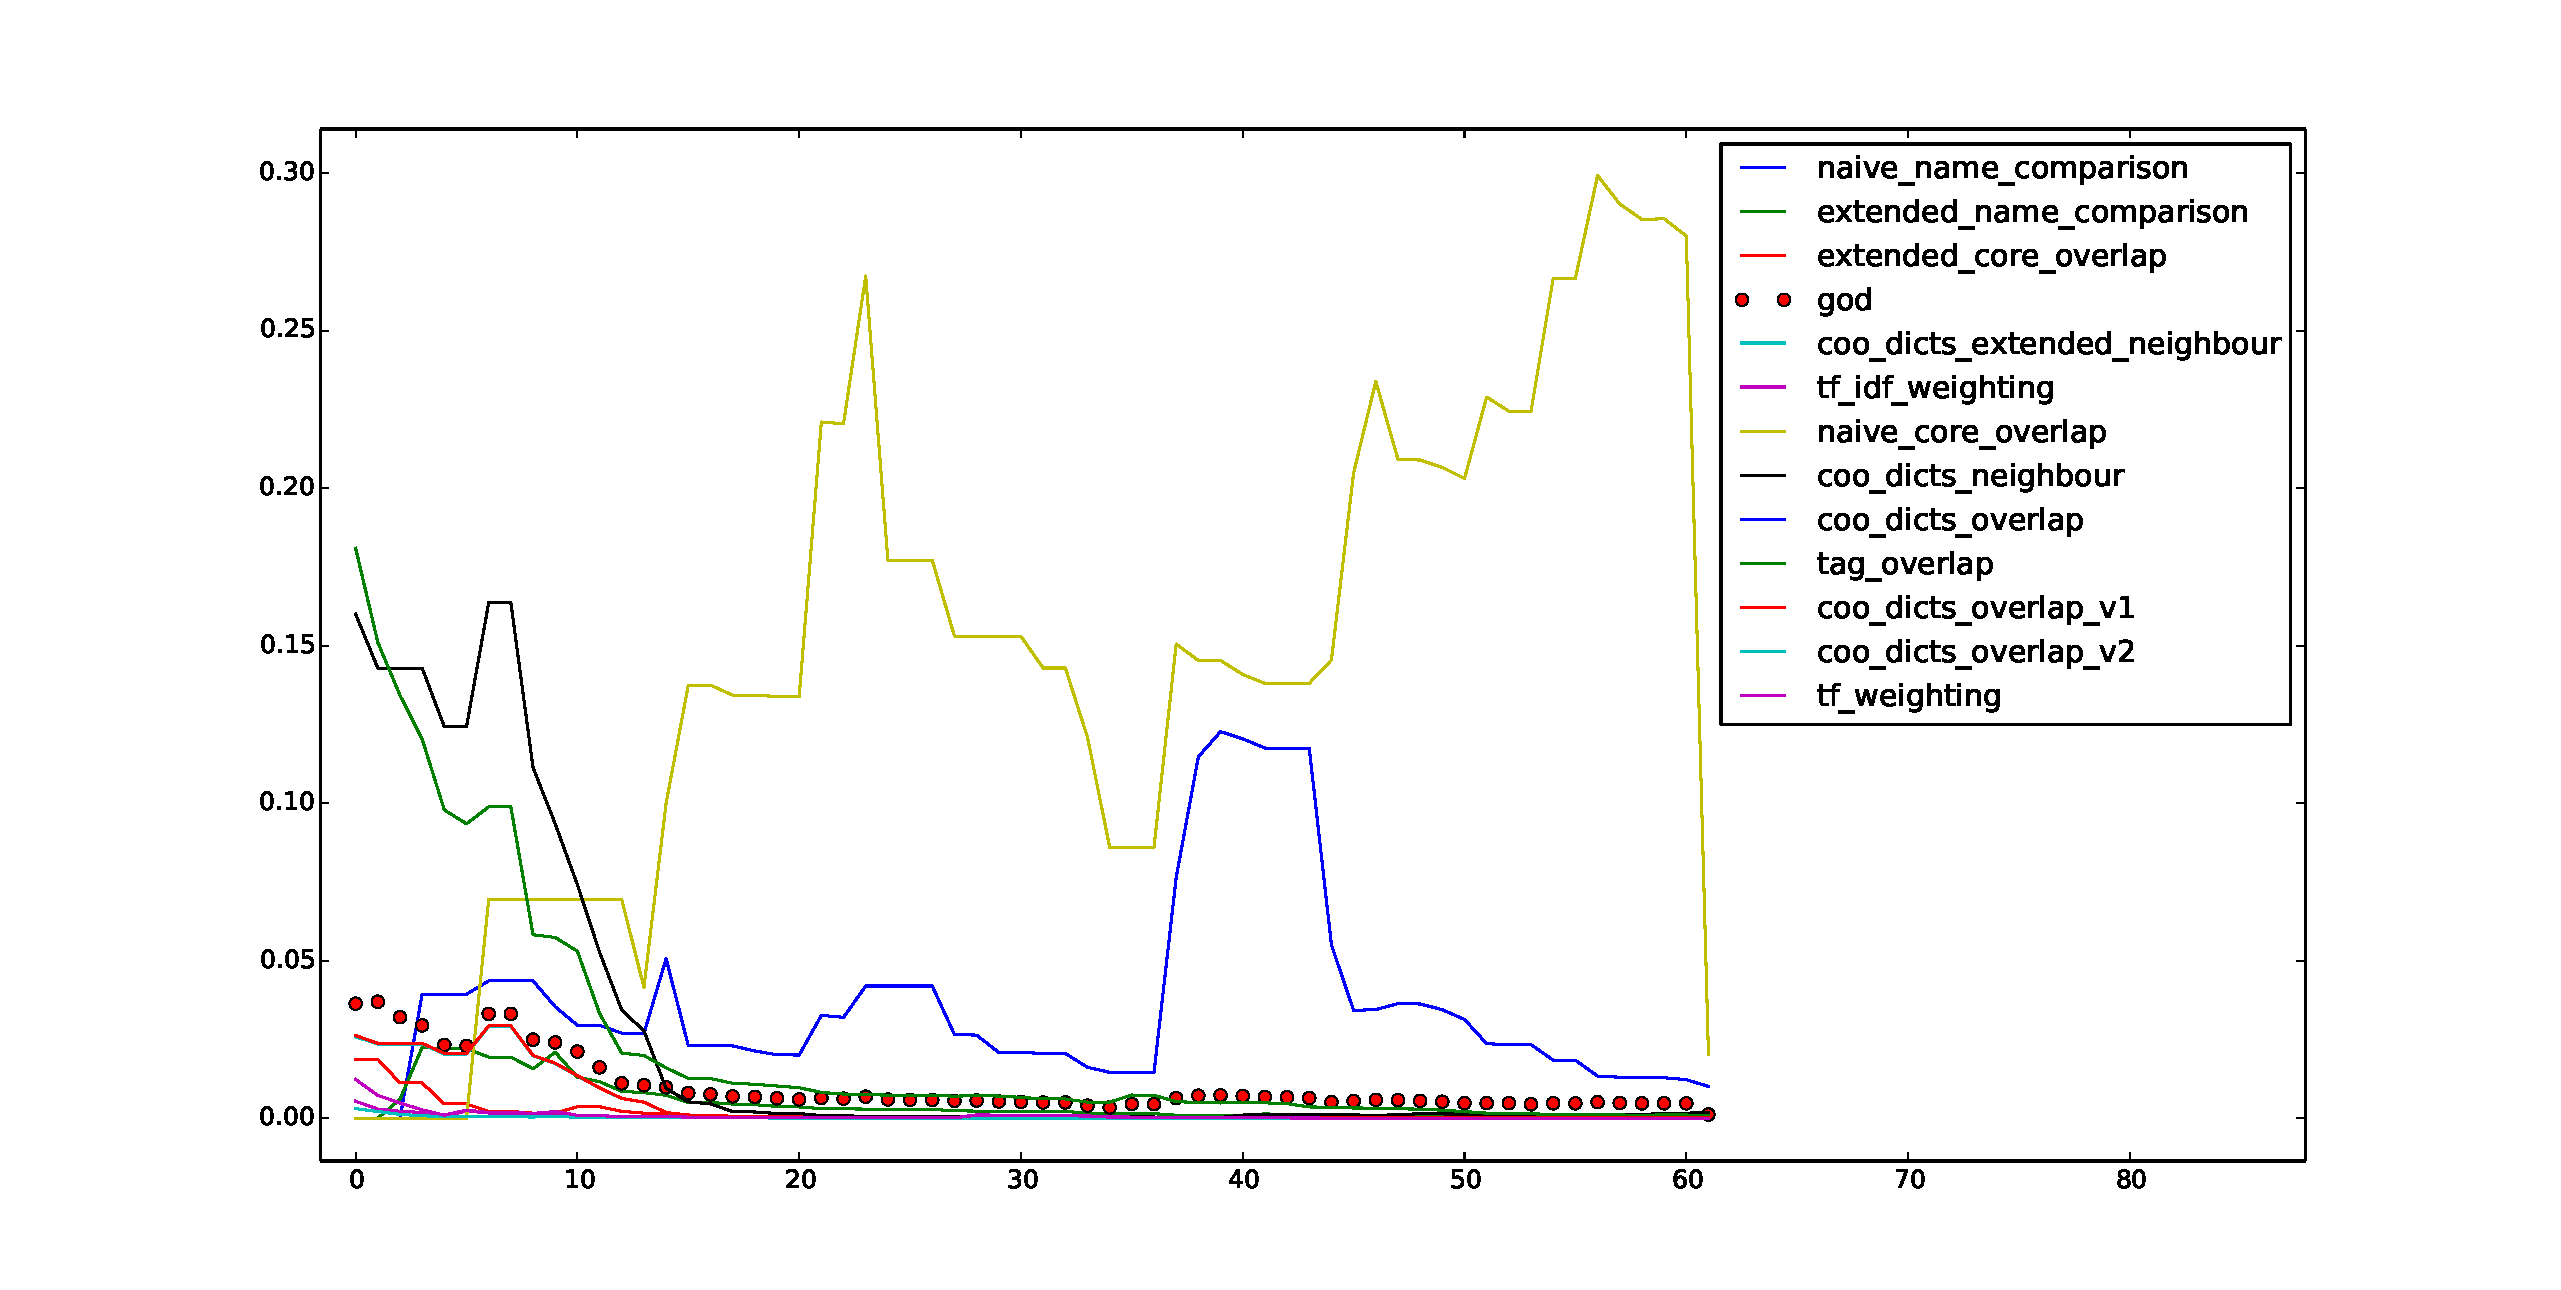
\includegraphics[width=\unitlength]{/home/pietro/Perceptum/code/starfish/similarity/SemanticSky/report_imgs/average_belief_in_true_links_median_lr05_punish_full.pdf}\hspace{-340pt} Figure \themyfigure : average belief in true links }%
  \end{picture}%
\endgroup%


\stepcounter{myfigure}
\def\svgwidth{500pt}
\begingroup%
  \makeatletter%
  \providecommand\color[2][]{%
    \errmessage{(Inkscape) Color is used for the text in Inkscape, but the package 'color.sty' is not loaded}%
    \renewcommand\color[2][]{}%
  }%
  \providecommand\transparent[1]{%
    \errmessage{(Inkscape) Transparency is used (non-zero) for the text in Inkscape, but the package 'transparent.sty' is not loaded}%
    \renewcommand\transparent[1]{}%
  }%
  \providecommand\rotatebox[2]{#2}%
  \ifx\svgwidth\undefined%
    \setlength{\unitlength}{1229.4bp}%
    \ifx\svgscale\undefined%
      \relax%
    \else%
      \setlength{\unitlength}{\unitlength * \real{\svgscale}}%
    \fi%
  \else%
    \setlength{\unitlength}{\svgwidth}%
  \fi%
  \global\let\svgwidth\undefined%
  \global\let\svgscale\undefined%
  \makeatother%
  \begin{picture}(1,0.50366032)%
    \put(-0.18,0){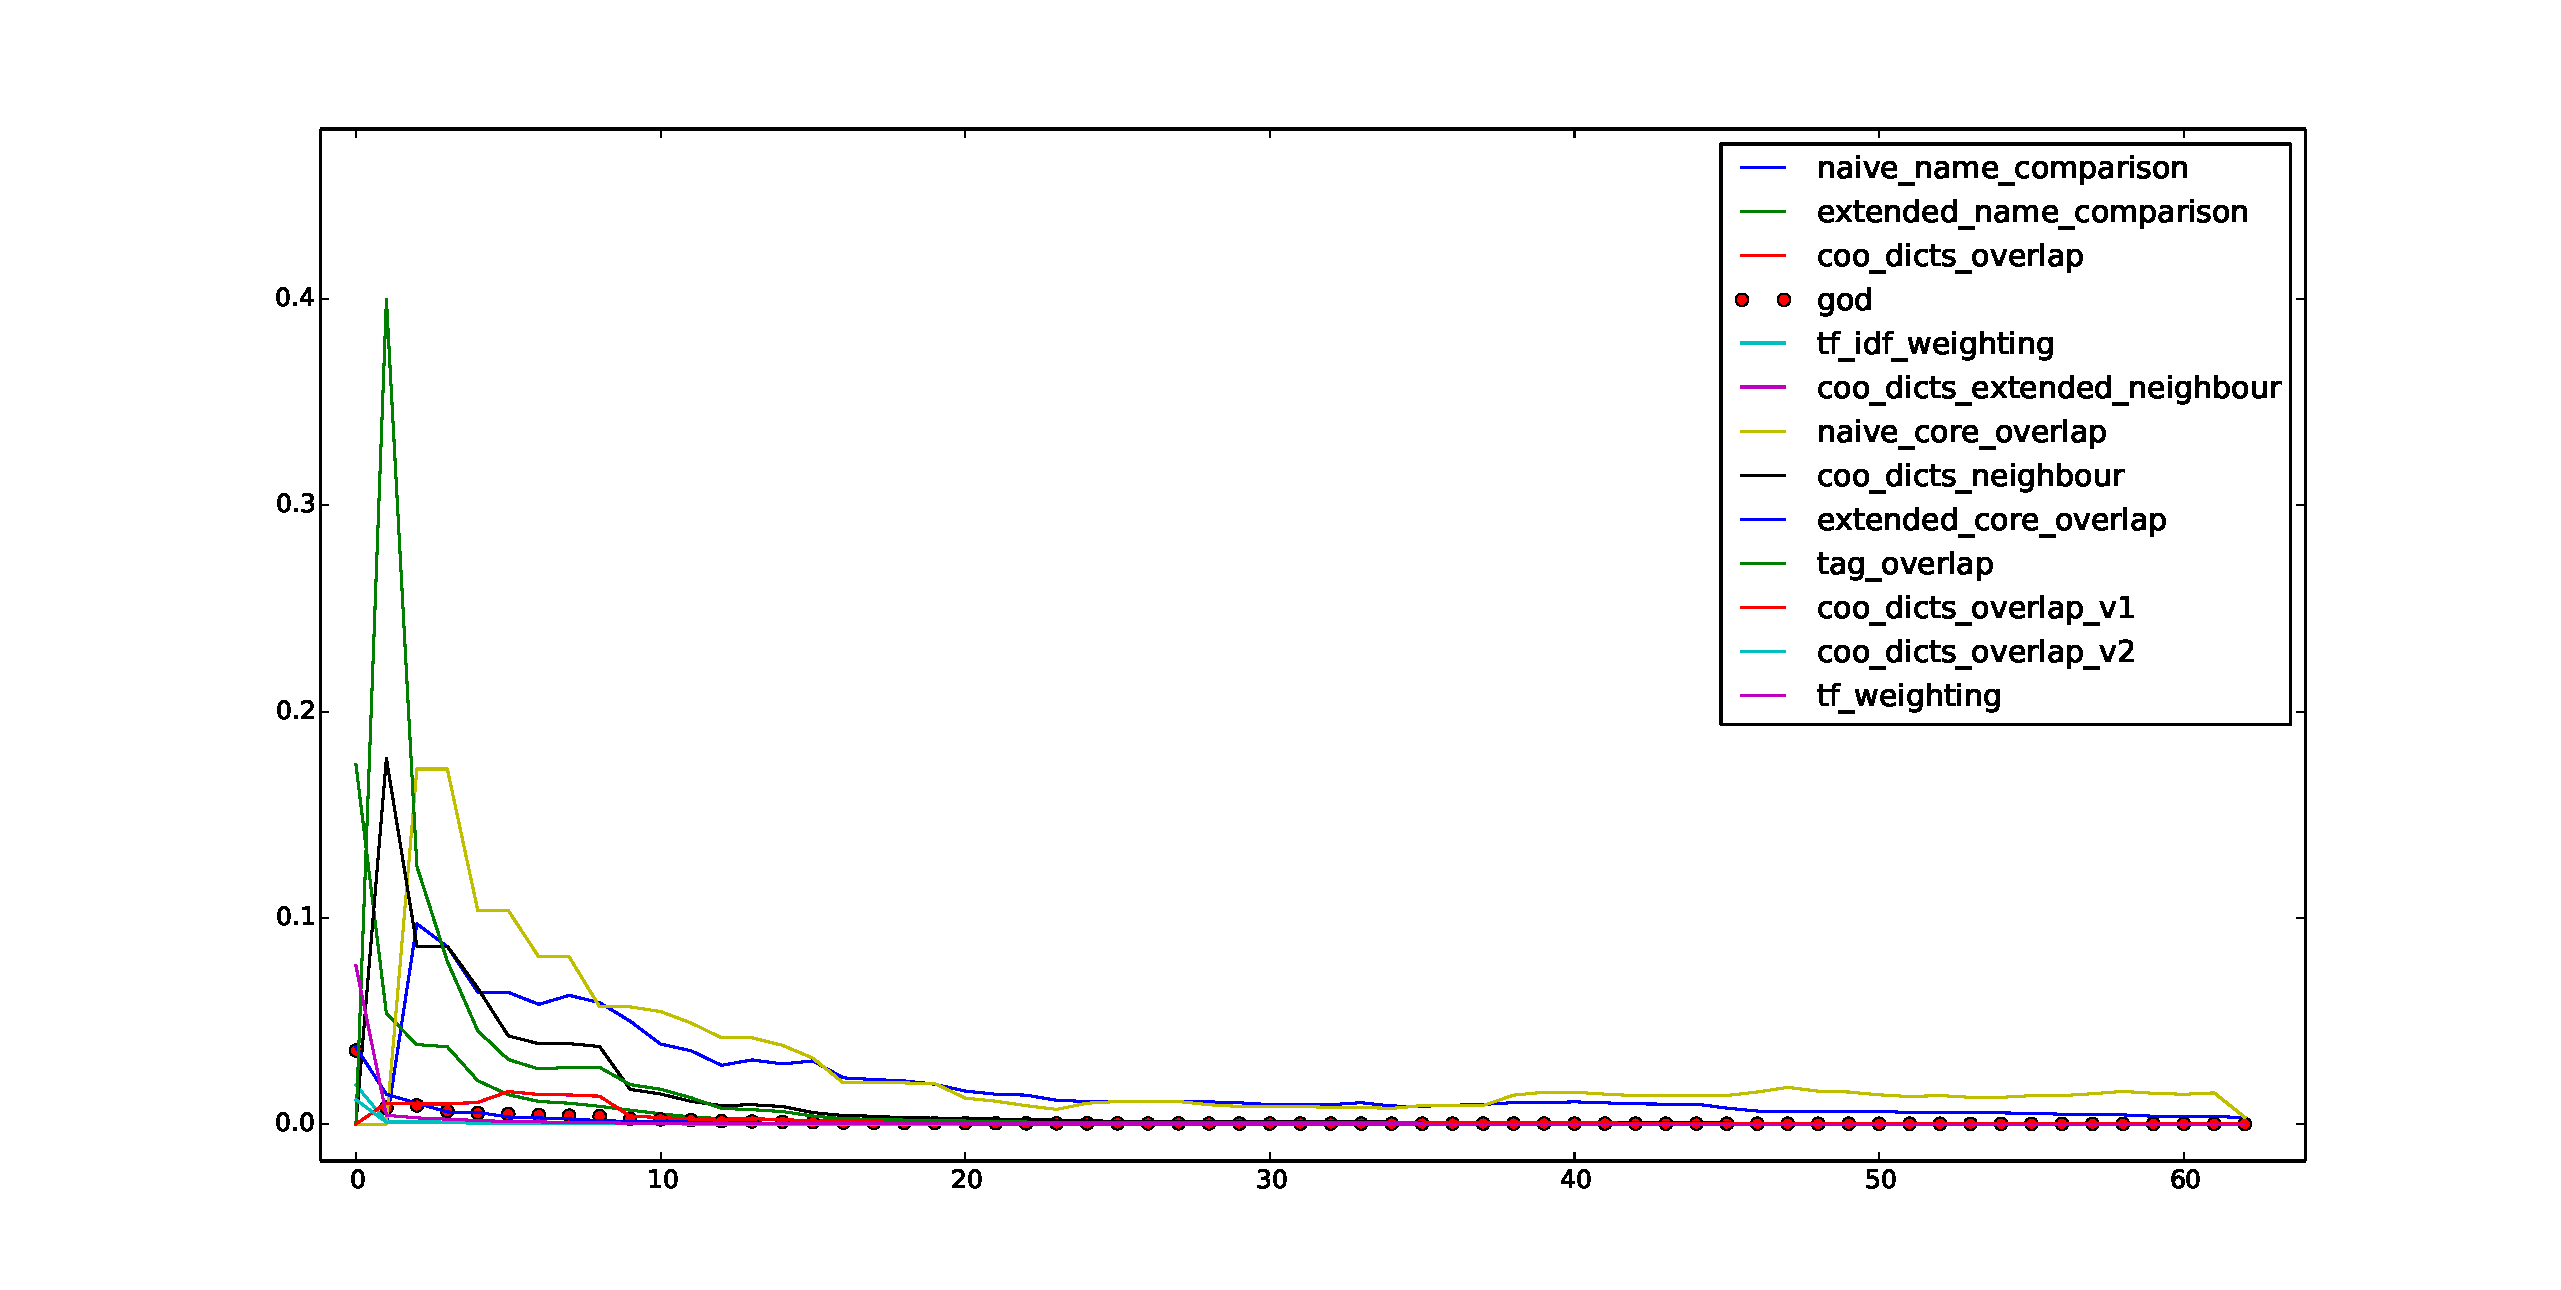
\includegraphics[width=\unitlength]{/home/pietro/Perceptum/code/starfish/similarity/SemanticSky/report_imgs/average_belief_in_false_links_median_punish_ls05_full.pdf}\hspace{-340pt} Figure \themyfigure : average belief in false links }%
  \end{picture}%
\endgroup%



\stepcounter{myfigure}
\def\svgwidth{500pt}
\begingroup%
  \makeatletter%
  \providecommand\color[2][]{%
    \errmessage{(Inkscape) Color is used for the text in Inkscape, but the package 'color.sty' is not loaded}%
    \renewcommand\color[2][]{}%
  }%
  \providecommand\transparent[1]{%
    \errmessage{(Inkscape) Transparency is used (non-zero) for the text in Inkscape, but the package 'transparent.sty' is not loaded}%
    \renewcommand\transparent[1]{}%
  }%
  \providecommand\rotatebox[2]{#2}%
  \ifx\svgwidth\undefined%
    \setlength{\unitlength}{1229.4bp}%
    \ifx\svgscale\undefined%
      \relax%
    \else%
      \setlength{\unitlength}{\unitlength * \real{\svgscale}}%
    \fi%
  \else%
    \setlength{\unitlength}{\svgwidth}%
  \fi%
  \global\let\svgwidth\undefined%
  \global\let\svgscale\undefined%
  \makeatother%
  \begin{picture}(1,0.50366032)%
    \put(-0.18,0){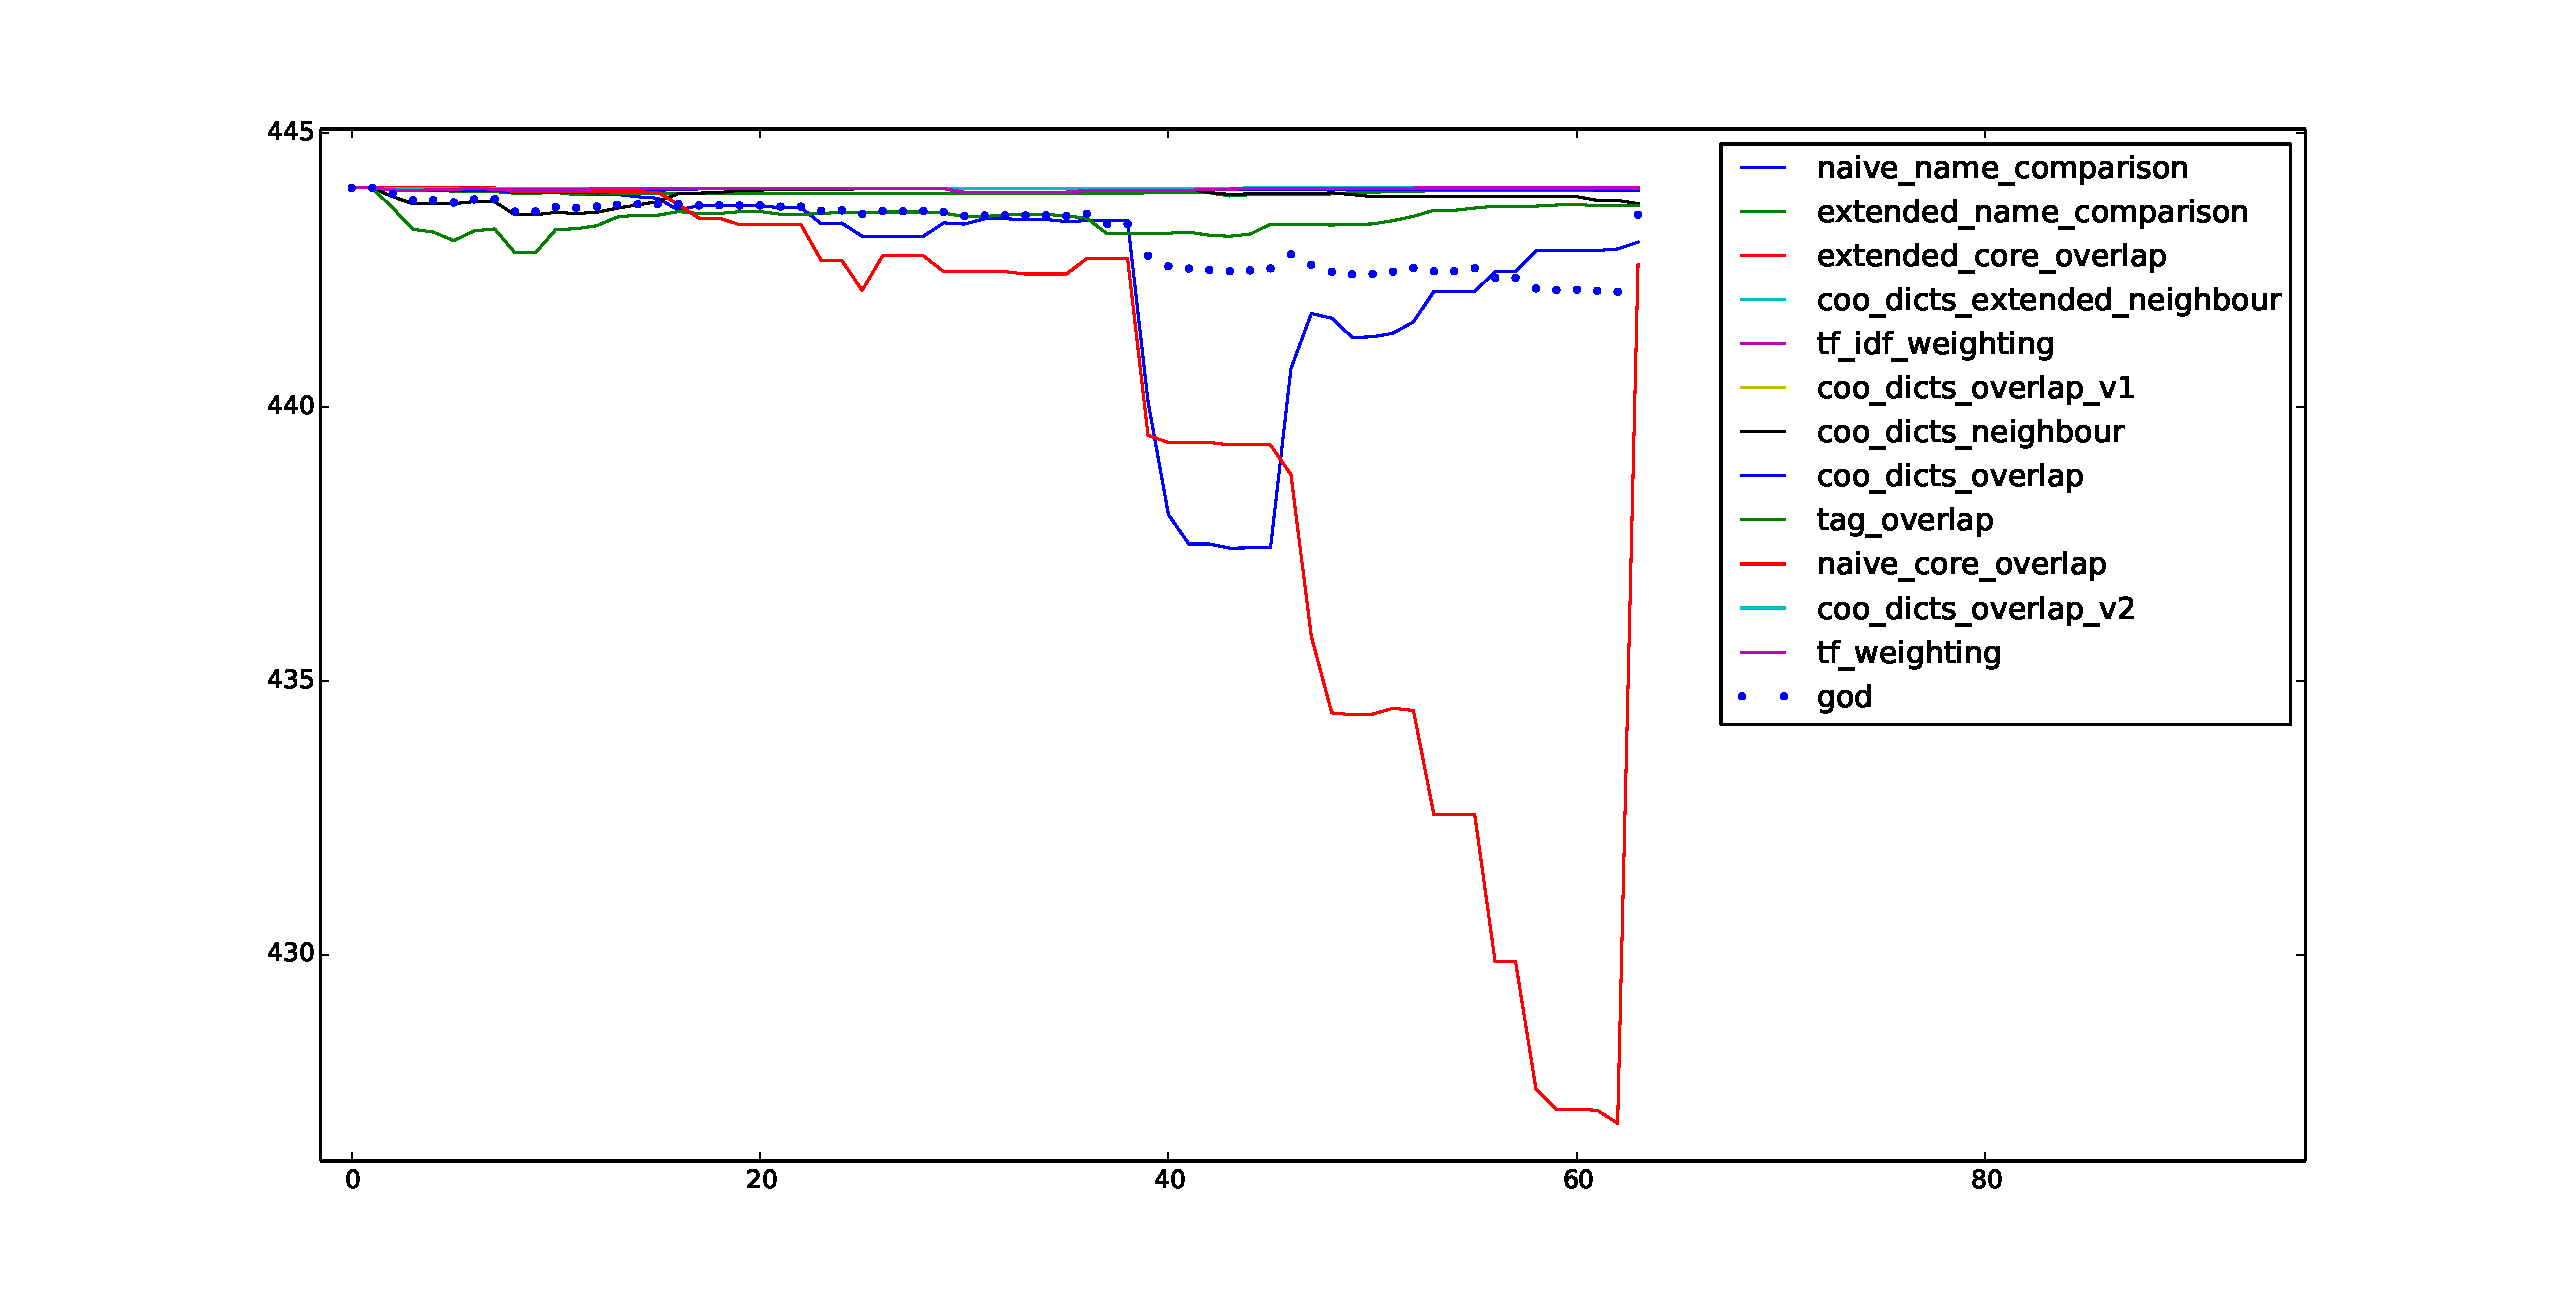
\includegraphics[width=\unitlength]{/home/pietro/Perceptum/code/starfish/similarity/SemanticSky/report_imgs/regret_of_angels_median_lr05_punish_fulltest.pdf}\hspace{-355pt} Figure \themyfigure : regrets only on true links}%
  \end{picture}%
\endgroup%
\vspace{5pt}
\clearpage
As before, the two following, final figures represent the outcome of a different test (on the present test): taking the weight sets as sampled during the evolution of god's beliefs as the present test (median, learning rate 0, punish) proceeded and assigning them to a different god, we have him refresh his belief set according to these weights and then plot the resulting regrets.

As you can see, also by comparing these figures to the previous (`healthy') ones, the regrets in this case touch the top (440) and seem stably hang to the asymptote. In the `all links' version of the regret calculation, on the other hand, we have an incredibly descending curve which stabilises at a very low value (1250 for God's regrets), against the 2000 top in the non-punish case(s).

This is due to the fact that all trustworthiness ratios go down, and thus, being most links false (i.e. not in Starfish) the angel's guesses get statistically more correct as their weighted value approaches 0. (This is also known as sample bias.)

Of course we would like regrets to decrease (especially where God is concerned), but as you can see from the graph displaying the evolution of regrets on true links, this is not happening in an altogether desirable way.



\clearpage






\stepcounter{myfigure}
\def\svgwidth{500pt}
\begingroup%
  \makeatletter%
  \providecommand\color[2][]{%
    \errmessage{(Inkscape) Color is used for the text in Inkscape, but the package 'color.sty' is not loaded}%
    \renewcommand\color[2][]{}%
  }%
  \providecommand\transparent[1]{%
    \errmessage{(Inkscape) Transparency is used (non-zero) for the text in Inkscape, but the package 'transparent.sty' is not loaded}%
    \renewcommand\transparent[1]{}%
  }%
  \providecommand\rotatebox[2]{#2}%
  \ifx\svgwidth\undefined%
    \setlength{\unitlength}{1229.4bp}%
    \ifx\svgscale\undefined%
      \relax%
    \else%
      \setlength{\unitlength}{\unitlength * \real{\svgscale}}%
    \fi%
  \else%
    \setlength{\unitlength}{\svgwidth}%
  \fi%
  \global\let\svgwidth\undefined%
  \global\let\svgscale\undefined%
  \makeatother%
  \begin{picture}(1,0.50366032)%
    \put(-0.18,0){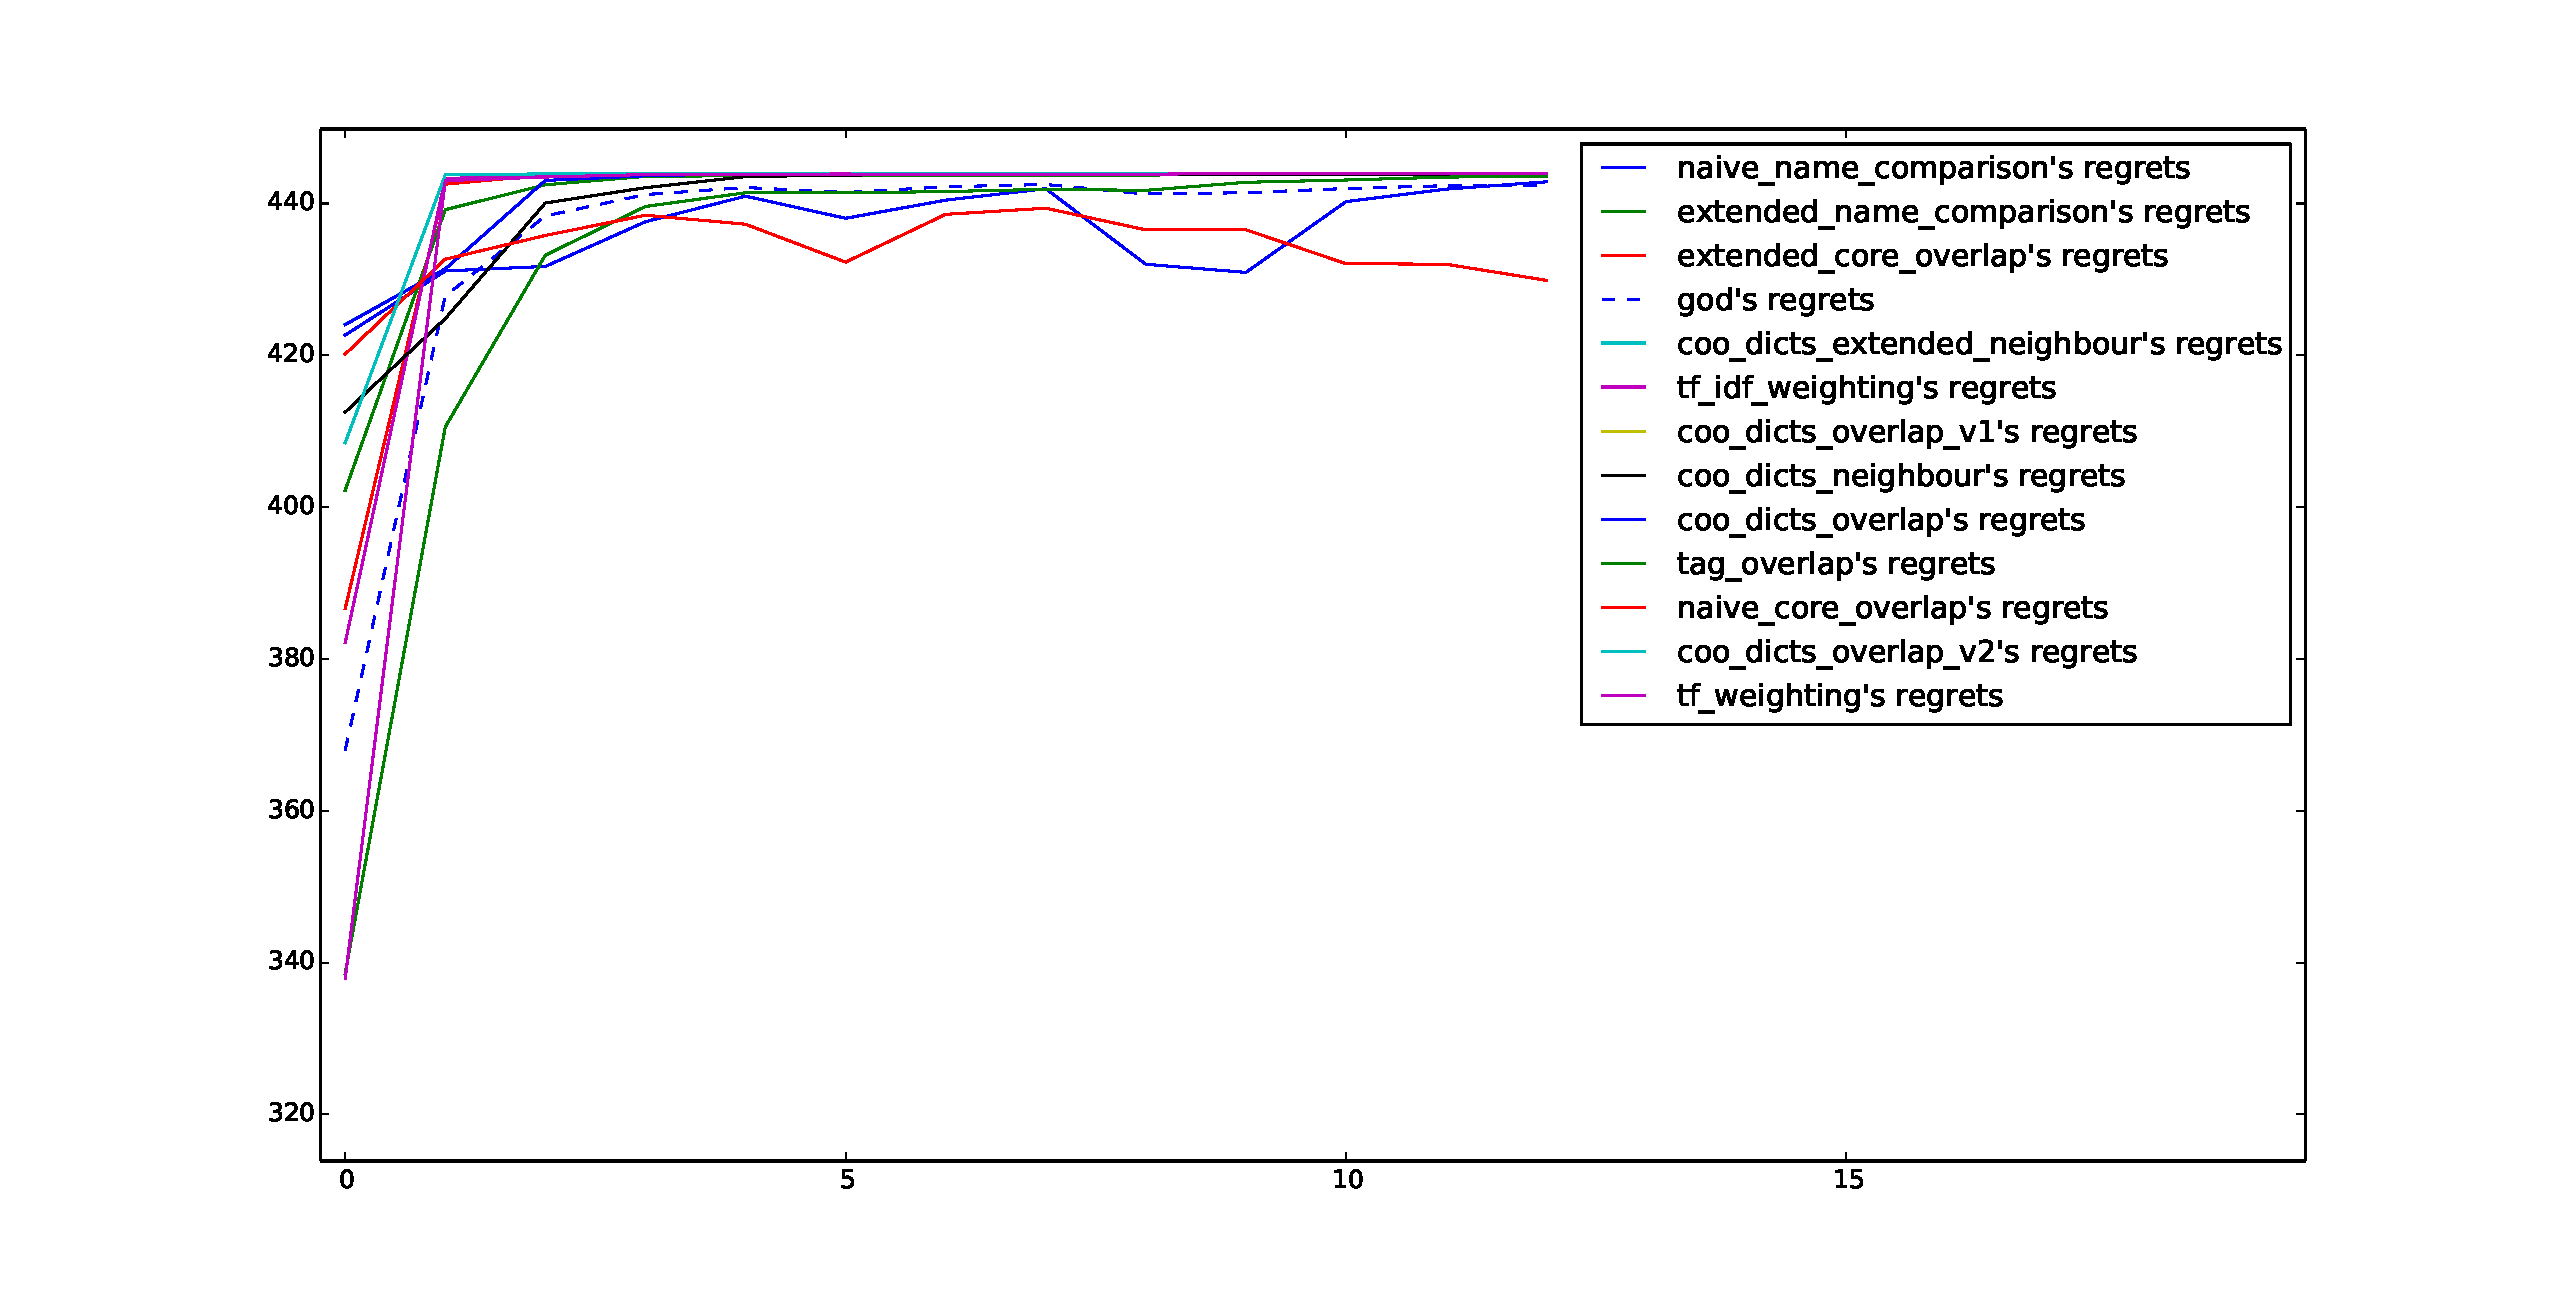
\includegraphics[width=\unitlength]{/home/pietro/Perceptum/code/starfish/similarity/SemanticSky/report_imgs/evolution_of_regrets_ontrue_median_punish_ls05_full.pdf}\hspace{-340pt} Figure \themyfigure : evolution of regrets (on true links) }%
  \end{picture}%
\endgroup%

\stepcounter{myfigure}
\def\svgwidth{500pt}
\begingroup%
  \makeatletter%
  \providecommand\color[2][]{%
    \errmessage{(Inkscape) Color is used for the text in Inkscape, but the package 'color.sty' is not loaded}%
    \renewcommand\color[2][]{}%
  }%
  \providecommand\transparent[1]{%
    \errmessage{(Inkscape) Transparency is used (non-zero) for the text in Inkscape, but the package 'transparent.sty' is not loaded}%
    \renewcommand\transparent[1]{}%
  }%
  \providecommand\rotatebox[2]{#2}%
  \ifx\svgwidth\undefined%
    \setlength{\unitlength}{1229.4bp}%
    \ifx\svgscale\undefined%
      \relax%
    \else%
      \setlength{\unitlength}{\unitlength * \real{\svgscale}}%
    \fi%
  \else%
    \setlength{\unitlength}{\svgwidth}%
  \fi%
  \global\let\svgwidth\undefined%
  \global\let\svgscale\undefined%
  \makeatother%
  \begin{picture}(1,0.50366032)%
    \put(-0.18,0){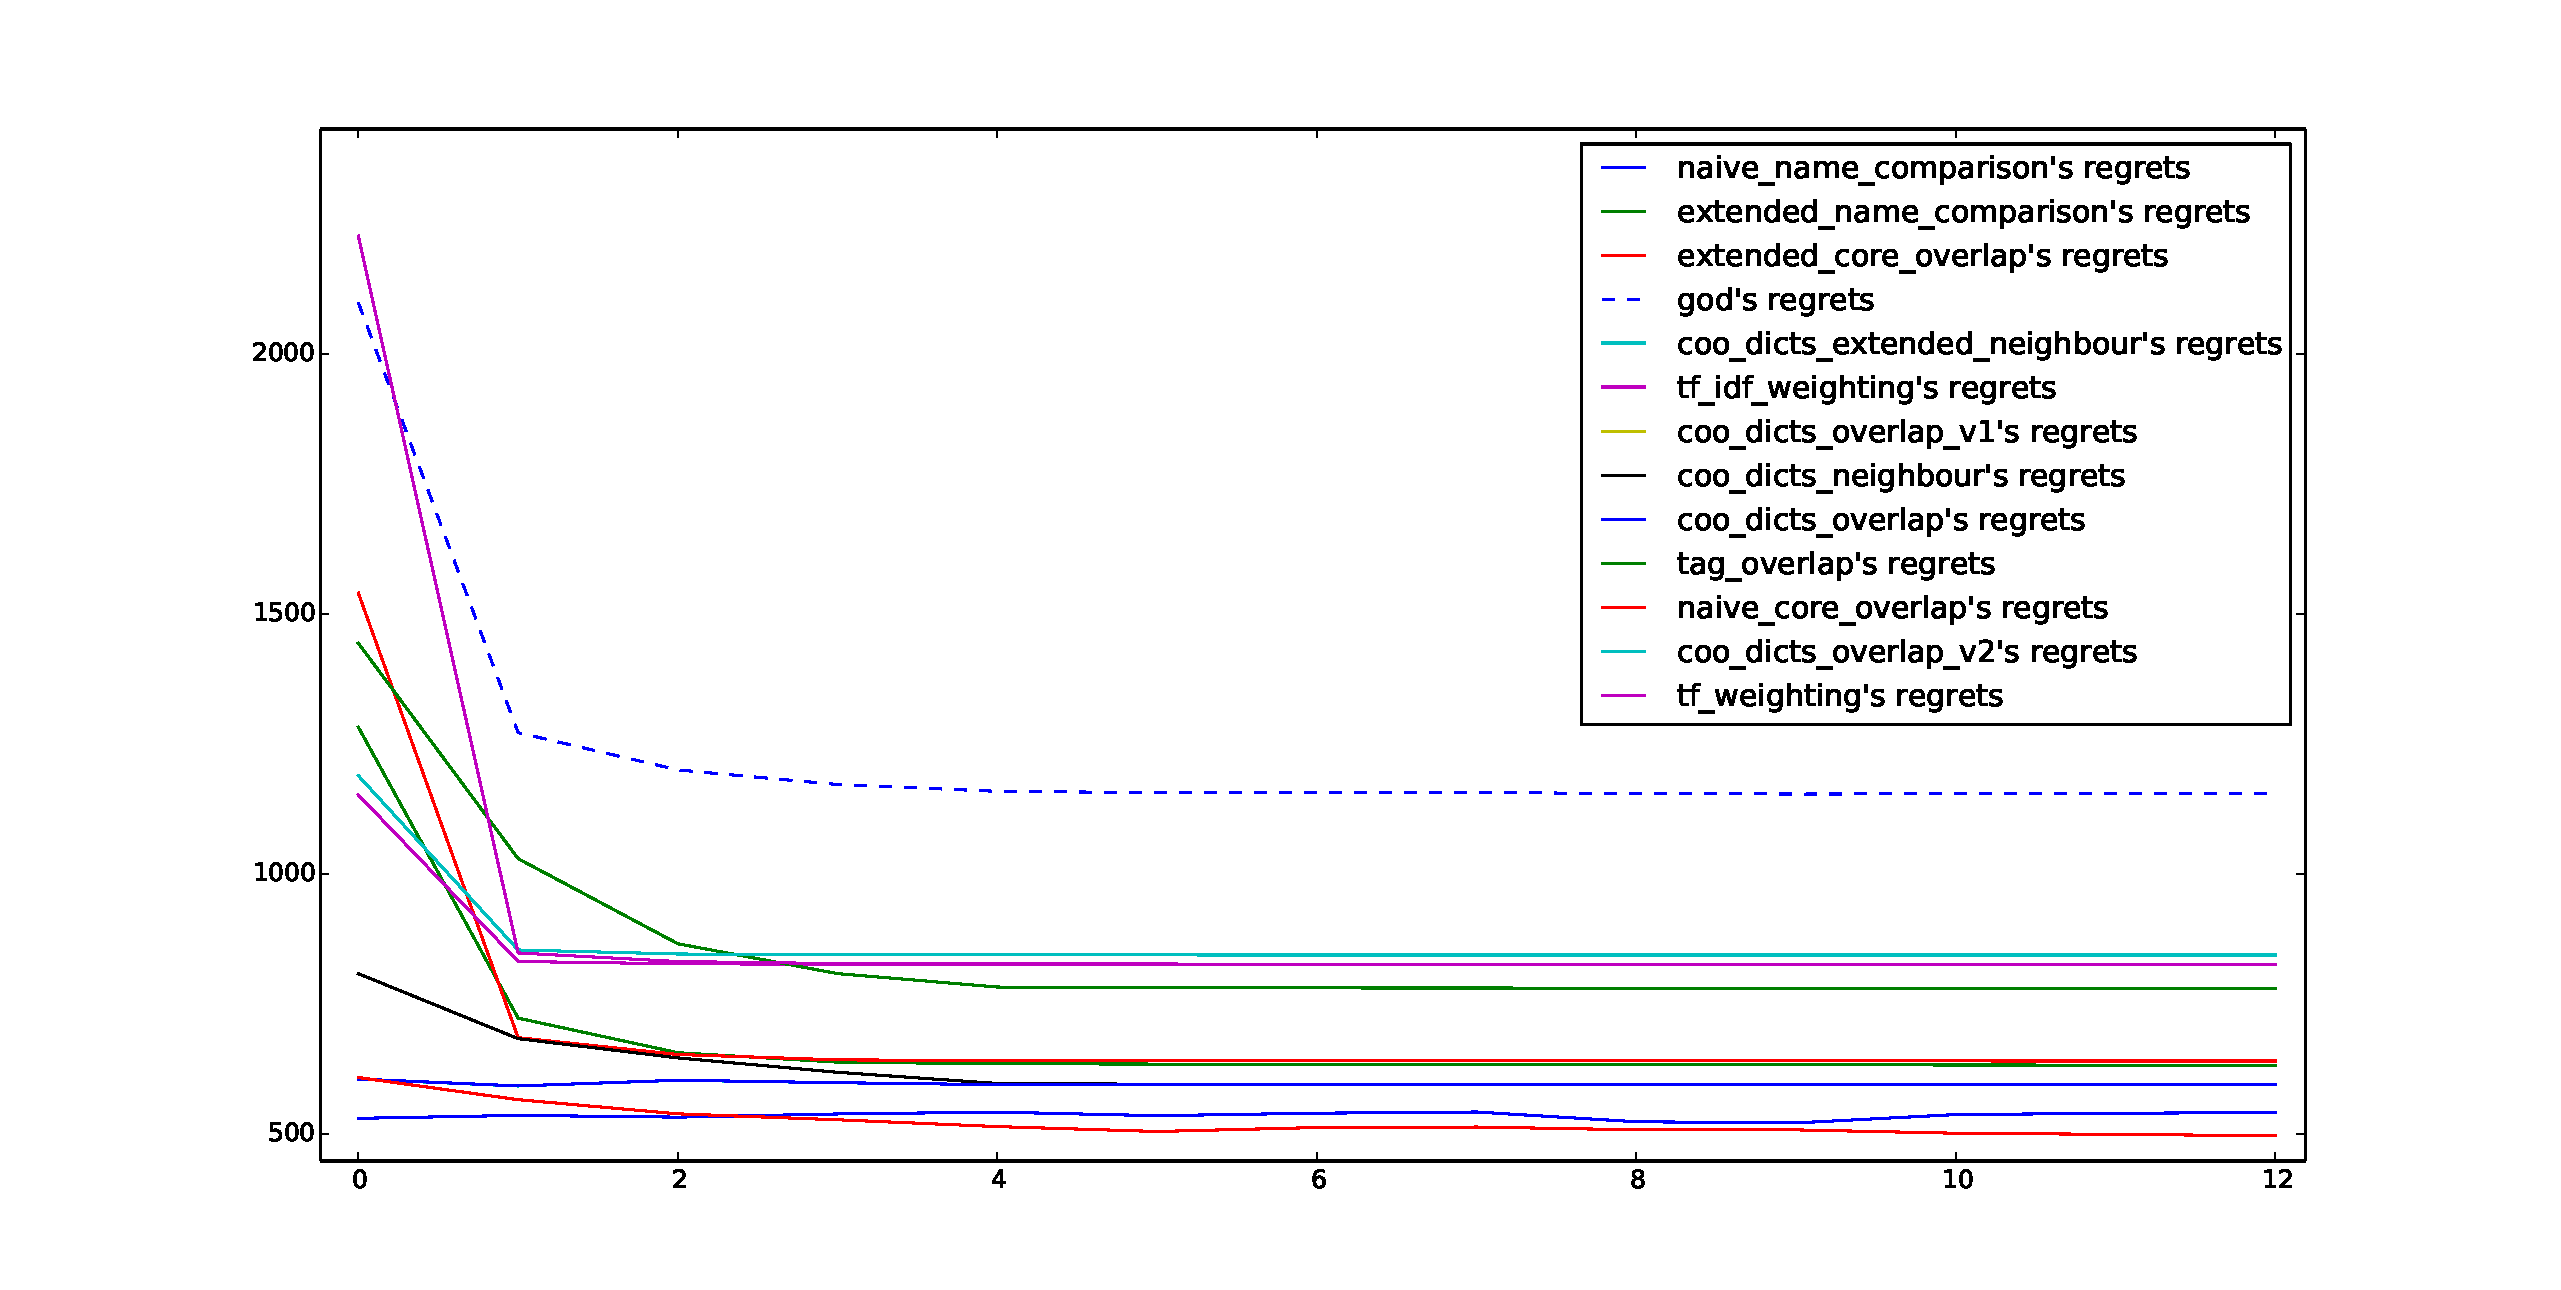
\includegraphics[width=\unitlength]{/home/pietro/Perceptum/code/starfish/similarity/SemanticSky/report_imgs/evolution_of_regrets_onall_median_punish_ls05_full.pdf}\hspace{-340pt} Figure \themyfigure : evolution of regrets (on all links) }%
  \end{picture}%
\endgroup%
\vspace{5pt}

Even though these graphs seem to argue definitely in disfavour of punishing false negatives, this bad performance might be due to the huge sample bias we have to face in Starfish.

Besides trying to compensate that in some ways (see next appendix), trying SemanticSky on a more balanced or simply bigger database will probably give more definitive results.





\subsection{Further testing: differentiating learning rates to counter sample bias and equalization to counter algorithms output bias.}

During the first round of testing, we noticed that there were two important problems that the framework was not able to cope with:
\begin{itemize}
\item a great sample bias (true links were 444, versus more than 21.000 false negatives in some cases).
\item what I will call \textbf{output bias}: most algorithms' normalization of the output produced an uneven distribution of values pushed towards zero. Thus, the distance between the average of the values which received positive feedback (meaning that the guess was correct) and the average of the values which received a false feedback were quite near. If we want to call `confidence ratios' the raw outputs of the algorithms, we can phrase the problem by saying that the confidence ratios were on average very low (the highest average for all the algorithms being 0.3, and the most of them leaning towards 0.05.).
\end{itemize}

To counter the first, we introduced differentiation of learning rates for positive and negative feedback.

To counter the latter, we tried to use what I will call an \textbf{equalizer}: a map from raw output of the algorithm to a more even distribution of values, evaluated online (or updated periodically) and eventually learned by the algorithms themselves, that tries to push apart the average of values that received a positive feedback and the average of these which received a negative one.

\subsection{Differentiation of learning rates.}
An option known in machine learning for its effectiveness is to use different learning speeds for positive and negative examples, diminishing the latter by a factor that depends on the size of the sample bias we face.

No testing was made in this direction, even though the code already includes this possibility, disabling it by default, mainly because at the moment, as you will already know, we just are not giving any feedback on negative examples. Beside taking too much time to run, punishing false negatives had some other cons you can find in the appropriate appendix.

\subsection{Equalization.}
The first experiments (as discussed in the central sections of this report) showed that between average confidence ratios in true and false items there was a gap, although maybe little. Thus, simple thresholding might have worked in pulling them apart.

We were hoping that through weighting of output / feedback, that gap would increase and be a more accurate division line between true and false links. Nonetheless, what typically occurred was that the weighting, which, you will remember, can only take down trustworthiness\footnote{And this, once more, is something to question.}, would push down all values. And being the evaluation spectrum [0/1], generally the values closer to 0 the positive pole (average of the values which received a positive feedback) would move down more than the negative one.

At the end of this process, the gap had in fact decreased. In this table, you can read to the left the name of the Guardian Angel and on the right the difference between the gaps before and after a full evaluation (and a full round of feedback). A positive value means that the gap has increased, but unfortunately you cannot see any. 
\vspace{5pt}

\begin{tabular}{l || c }
angel & polar gap on weighted beliefset \\
\hline
coo\_dicts\_extended\_neighbour & -0.00201 \\
 coo\_dicts\_neighbour &-0.012\\
 coo\_dicts\_overlap & -0.0037\\
 coo\_dicts\_overlap\_v1 & -0.00202\\
 coo\_dicts\_overlap\_v2& -0.0037\\
 extended\_core\_overlap& -0.027\\
 extended\_name\_comparison& -0.017\\
 naive\_core\_overlap& -0.21\\
 naive\_name\_comparison&  -0.15\\
 tag\_overlap&  -0.036\\
 tf\_idf\_weighting&  -0.014\\
 tf\_weighting&-0.039\\
 \hline
 god &-0.032 \\
\hline
sum (including god) & -0.548
\end{tabular}

\vspace{5pt}

Overall, the decrease rate of the gap is not so high, but if this is not evidence that something is wrong, then few other things could be.

% IDEA: we take the unweighted average belief in true/false links and map it to the equalized and to the weighted, in this order
% numerical measurement: the distance between the points at the various steps. Ideally it should increase! so, - distance at step 1 + distance at step 2 should be POSITIVE. The bigger the better.
%
%
%
%
%
%
%





With equalization (and an experiment with the same parameters), this is what we have:

\vspace{5pt}

\begin{tabular}{l || c | c | c}

angel & equalization & weighting & overall \\
\hline
coo\_dicts\_extended\_neighbour & 0.00074 & -0.0019 & -0.0012\\
 coo\_dicts\_neighbour & -0.0081 & -0.0102&-0.018\\
 coo\_dicts\_overlap & 0.0039 & -0.004&-0.000104\\
 coo\_dicts\_overlap\_v1 & 0.00077& -0.0019 & -0.0012\\
 coo\_dicts\_overlap\_v2& 0.0039& -0.004 & -0.000104\\
 extended\_core\_overlap& 0.0075& -0.033& -0.025\\
 extended\_name\_comparison& 0.032& -0.025 &0.0076\\
 naive\_core\_overlap& 0.0012& -0.21 &-0.21\\
 naive\_name\_comparison& 0.00069& -0.15 &-0.15\\
 tag\_overlap& 0.018& -0.042& -0.023\\
 tf\_idf\_weighting& 0.0301& -0.018 & 0.011\\
 tf\_weighting& 0.038& -0.0506 & -0.011\\
 \hline
 god& & & -0.032 \\
\hline
sum (including god) & & & -0.453
\end{tabular}
\vspace{5pt}

The middle column is the step from the raw evaluation to the equalized evaluation, the right column is the step from the equalized evaluation to the final state of the belief set: that is, the weighted (by contextual trustworthiness) and equalized belief set.

As you can see, equalization manages in all but one case (where the algorithm is \emph{so} bad that its average confidence in correct suggestions is lower than the that in wrong ones) to widen the gap between the poles. The problem is that then weighting manages to destroy that effort. Maybe this could be countered by making equalization heavier (the curve was very flat close to the centre of gravity of the push, and unfortunately that's precisely where most values are!), but maybe this is just not working.

In most cases, the overall value (gap difference between unweighted, unequalized and weighted, equalized belief sets) is still negative, which means that the gap is decreasing. We can see however that except for a few examples (still too many, maybe) equalization has managed to reduce a bit (still too little, probably) the negative squeezing effect of weighting (look at the `sum' lines: more or less one fifth effect decrease).

Besides, it's questionable (though it seemed quite natural to us) the order we chose for the pipeline: we might as well equalize up the weighted beliefset, instead of weighting down the equalized beliefset. Who knows what might happen.

More experimentation and research are needed to draw more definitive conclusions here, but we think that this equalization business is probably going in the right direction, but just `not enough' to solve all of our problems, including the weather.

















\end{document}